% $Id: paper.tex 785 2005-06-16 15:51:29Z hussain $

%\documentclass{sig-alternate}
\documentclass{sig-alt-nocopy}
% to go back to 9pt, do sig-alt-nocopy
%\documentclass{sigplan-proc-10pt}

% hack to avoid the ugly ACM paragraph definition
% => can't leave blank line after this
\renewcommand{\paragraph}[1]{\vskip 6pt\noindent\textbf{#1 }}

%
% Kannan's suggestions about maximizing floats:
% (images)
%
\newcommand{\RelaxFloats}{
	\renewcommand{\topfraction}{0.9}
	\renewcommand{\floatpagefraction}{0.9}
	\renewcommand{\textfraction}{0.1}
}
\RelaxFloats


\usepackage{epsfig}
\usepackage{times}
\usepackage{xspace}
\usepackage{url}
\usepackage{dcolumn} % see Gossens et al p 129
\usepackage{multirow}
\usepackage{rotating}
\usepackage{graphicx}
\DeclareGraphicsRule{.idraw}{eps}{.idraw}{}
\usepackage{subfigure}
\usepackage{endnotes}

\newcommand\comment[1]{{[\sffamily #1]}}

%\pagenumbering{arabic}
\begin{document}

% Attempt to get latex to put the figures where we want them
\renewcommand{\topfraction}{0.85}
\renewcommand{\textfraction}{0.1}
\renewcommand{\floatpagefraction}{0.75}

%\pagenumbering{arabic}
% For camera ready submission we may have to put in what page this appears
% in the proceedings.
%\setpagenumber{9}

\title{A Comparative Study of Network Testbed Usage Characteristics
}

\newcommand{\FromA}{\raisebox{8pt}{$\dagger$}}
\newcommand{\FromAB}{\raisebox{8pt}{$\dagger\ddagger$}}

\numberofauthors{1}
\author{
\alignauthor Jelena Mirkovic, Hao Shi, Alefiya Hussain \\
 \affaddr USC/Information Sciences Institute \\ 
 \email{mirkovic,haoshi,hussain@isi.edu}
}

\maketitle

\abstract


\section{Introduction}
\label{sec:intro}
\section{Related Work}
\label{sec:related}
\section{Background}
\label{sec:terms}

We define a \textit{network testbed} as any collection of physical or
virtual machines that is shared by multiple users with the goal to
support research or education activities. This is a broad definition
that encompasses Emulab-like testbeds such as Emulab \cite{emulab} or
DETER \cite{deterlab} where users gain exclusive, superuser access to
physical nodes, VM-based testbeds such as Planetlab \cite{planetlab}
where multiple users share access to a physical node and private
testbeds in research labs and companies. The goal of this paper is to
understand how network testbeds are used and to identify places where
improvements are needed.

Discuss how testbeds differ and their modes of use. Discuss project,
slice, experiment, etc. Say experiments and projects have descriptions.
We will show mapping as we go and in a table.

Say how we lack info about what users do with machines.

\subsection{Testbed Uses}

Two main testbed use modes we investigate in this paper are for research
and for classes. In research use model a group of users investigates a
common research problem and uses testbed to evaluate the problem or
their solutions. The users could be from academia (faculty and
students), a government lab (researchers, staff)  or industry (company
employees). Their final goal may be to produce research papers, white
papers, to change government policies or to test a product. This variety
of research users makes it difficult for testbed owners to evaluate the
productivity of their users, ultimately quantifying how useful testbeds
are for research, because some research outcomes may not be public. In
classes teachers use testbeds to either illustrate a concept taught in
class or to assign a practical project to students. This project may be
of research nature, especially for upper division graduate classes,
which blurs the line between class and research.

\subsection{Terminology} \label{terminology}

An \textbf{experiment definition} is the input submitted to the testbed
(one or more times) describing resource needs and setup operations. The
experiment definition is closely tied to \textit{one particular
purpose}, e.g. a research question or a class project. It is uniquely
identified by its name and can be modified while still keeping its
identity.

An \textbf{experiment instance} denotes the combination of experiment
definition and testbed resources allocated to it. Return of the
resources to the testbed denotes the end of this instance. On the other
hand, a modification of the experiment definition which requires release
and reallocation of resources (e.g. to change experiment topology or add
more nodes) still belongs to the same instance. Thus an experiment
instance may be associated with more than one resource set.

A \textbf{project} is a collection of experiment definitions and people,
under a single Principal Investigator (PI) aiming to investigate one
specific research direction or taking one specific class.

%Put picture here to illustrate definition vs instance and changing size

In our investigation of testbed use patterns we have discovered a broad
range of activity levels in every dimension. Some projects and some
users were very active, while others generated none or a few experiment
instances. Some experiment instances were long-lived (months) while
others were extremely short (under 10 minutes). From pure use pattern
data it was impossible to understand the causes of such broad range of
uses. To disambiguate and possibly explain this data we have attempted
to somehow quantify from project descriptions, experiment definition
descriptions, personal conversations with the PIs and publications
co-authored by project members how useful the testbed was for each given
project. We could do so only for DETER data as the data we have from
other testbeds is anonymized due to privacy concerns.

The next several definitions apply to any testbed.

An \textbf{experiment manipulation} is any interaction between the user
and the testbed's control server. It usually results in allocation or
deallocation of testbed resources, either physical resources or database
entries.

An \textbf{active project} is a project associated with at least one
experiment manipulation. Similarly an \textbf{active user} is a user
that has manipulated at least one experiment. The rest of the projects
and users are labeled \textbf{inactive}. Further, users that do not
belong to any project are labeled \textbf{orphan users}. While it is
possible for an inactive but non-orphan user to still do some useful
work with the testbed, e.g., by logging into an experiment instance
allocated by another member of its project, orphan users cannot do any
useful work on the testbed.

We now introduce a few more definitions so we could attempt to separate
those projects and users where we see little associated activity due to
their short presence on the testbed from those where low activity is
related to poor match of the testbed with their research needs

A \textbf{warm-up time} is the time elapsed between a project's creation
and the first experiment manipulation.

%An \textbf{early project} is a project that has been present on the
testbed for less than a year. Similarly an \textbf{early user} is a user
that has been present on the testbed (has an account) for less than a
year. We have selected the threshold value of a year by observing the
distribution of warm up time for \textit{those research projects that
resulted in measurable outcome acknowledging DETER use (aka ``outcome
projects'', see below)}. This distribution is shown in Figure
\ref{warmup}. The highest warmup time we see is a little below 8 months.
To be conservative we select 1 year as the threshold for the project to
become active.

%A \textbf{stale project} is a project that is not early and is not
active. Similarly a \textbf{stale user} is a user that is neither early
nor active.

We further divide active projects on DETER into several categories. As
mentioned above, due to privacy concerns, we cannot perform similar
classification for projects on other testbeds. \begin{enumerate} \item
\textbf{Internal projects} are those projects created for monitoring and
development of DETER testbed. \textbf{Internal users} are those that are
members of any internal project. While many of those users also lead
research projects on DETER we have found through manual investigation
that PIs have hard time separating their activities into multiple
projects, i.e. some internal projects may be used to do research about
topics unrelated to the DETER testbed and vice versa. To avoid bias in
our data, since internal users have vested interest in the testbed and
are likely to be very active, we exclude both internal projects and
internal users from all DETER statistics. % We actually do this for
Emulab as well. We do not exclude them for project size/activity
calculation \item \textbf{Outcome projects} are those projects where we
can clearly attribute some measurable outcome of the project to its use
of DETER. We classify research projects as outcome projects if they have
produced at least one peer-reviewed publication (this includes MS and
PhD thesis), which acknowledges use of the DETER testbed. We classify
class projects as outcome projects if they have more than three members
(one PI and two TAs),  which indicates that students taking the class
have used DETER for their class work. There is one project that has 8
users and we classified it as no-outcome because we know these are PIs
exchanging materials. We selected the threshold value of three members
empirically. The rest of the projects are labeled as \textbf{no-outcome
projects}. \item \textbf{Try-and-leave projects} are those no-outcome
projects that have created a small number of experiment instances,
followed by at least a year of inactivity and where descriptions of
experiment instances suggest attempts to learn about the testbed (e.g.
``learning how to use DETER'',``trying out SEER''). We believe that this
use pattern indicates that the testbed did not match the users' needs.
\item \textbf{Hard-to-tell projects} are those that do not fall into
either of the above categories. That is, they exhibit usage patterns
that are suggestive of performing research of developing class materials
with DETER but they have not yet generated a measurable outcome. In case
of research projects there are many reasons for this effect. First, some
research may take years to mature to publication, i.e. it may just be
too early to tell. Second, the project may be industrial or government
project and thus we cannot expect it to produce a peer-reviewed
publication output. Since we know project and user affiliations on DETER
we can identify such projects (and we do later in text). Third, some use
of the testbed may generate negative results, e.g., a user believed he
could test some hypothesis on the testbed but concluded otherwise.
\end{enumerate}

% Add figure to show project classes and user classes
\section{Testbed Data}
\label{sec:data}


Authors are closely involved with the DETER testbed
\cite{deter} and a lot of data presented in this paper is derived from
monitoring DETER usage. As such some of our conclusions may apply just
to the DETER testbed or to Emulab-like testbeds. Where possible we
supplement our study with data from other testbeds, specifically Emulab,
Schooner, Planetlab and Starbed. This data is not entirely compatible
with data we have from DETER for three reasons: \begin{enumerate} \item
Due to privacy reasons other testbeds could not share with us data
identifying their users and projects. \item Use model of Planetlab and
Starbed is much different than use model of Emulab-like testbeds so it
is difficult to establish a mapping between units of work between
different testbeds. \end{enumerate} In the text we clearly identify
which data we used for our investigation and where and how our
conclusions apply.

Here is all the data we have: \begin{enumerate} \item DETER: Data about
each user, their affiliation and experiment manipulation activity. Data
about project topics, project membership and experiment manipulation
activity. Experiment durations. We have the preceding data from 2004
till today. Experiment topologies - only current snapshot for
experiments that are not terminated. Machine allocations to experiments
and activity (coarse-grained) for the past 6 months only. Data about
publications that we can link back to projects. % Failed swapin data
\item Emulab: Publicly available data about project topics and project
activity (coarse grained: some vs none). Data about user and project
activity (anonymized) and experiment sizes and durations. From 2002 till
today. %Publication data. \item Schooner: Data about each user, their
affiliation and experiment manipulation activity (coarse grained, no
data about experiments). Data about project topics, project membership
and experiment manipulation activity (coarse grained, no data about
experiments). \item Planetlab: Data about allocations and resource usage
for each project. \item Starbed: User resource reservations.
\end{enumerate}


\subsection{Privacy and Anonymization} 
Emulab data is anonymized, we know class and research classification 

PlanetLab data is anonymized, we know only sliceid 





\subsection{Cleaning the data}

Table \ref{cleaning} shows the breakdown of projects and users per
categories introduced in section \ref{terminology} for DETER and Emulab
data.

\begin{table}[htdp] \begin{center} \begin{tabular}{|c|c|c|} \hline
Projects & DETER & Emulab \\ \hline Total & 234 & 736 \\ Active & 179
(76\% of T) & 534 (76\% of T) \\ Active no alloc & 2 & 15 \\ Inactive &
55 & 202 \\ Early$*$ & 30 (55\% of I) & 150 (74\% of I)\\ Stale$*$ & 26
& 72 \\ Internal and active & 12 (7\% of A) & 25 (5\% of A)\\ Working
set  & 167 (93\% of A) & 509 (95\% of A)\\ Class & 34 (20\% of WS) & 42
(8\% of WS) \\ Outcome (class) & 25 (74\% of C) & 35 (83\% of C)\\
Research & 133 (80\% of WS) &  467 (92\% of WS)\\ Outcome (research) &
46 (35\% of R) & \\ \hline Users & DETER & Emulab\\ \hline Total & 2,345
&  3,607 \\ Orphan & 245 (10\% of T) & 210 (6\% of T)\\ Non-orphan &
2,100 & 3,397\\ Active & 1,579 (75\% of NO) & 1,966 (58\% of NO)\\
Inactive & 521 & 1,432 \\ Early$*$ & 463 (89\% of I) & 1,292 (90\% of
I)\\ Stale$*$ & 98 & 674 \\ Internal &  73 (5\% of A) & 194 (10\% of
A)\\ Working set  & 1,506 (95\% of A) & 1,772 (90\% of A)\\ Class &
1,132 (75\% of WS) & 443 (25\% of WS)\\ Research & 356 (24\% of WS)  &
1,267 (72\% of WS)\\ Mixed & 18 (1\% of WS) & 62 (3\% of WS)\\ \hline
\end{tabular} \end{center} \label{cleaning} \caption{Breakdown of
project and user data per category. Starred rows are generated by taking
the maximum warmup time for working-set projects/users as a threshold
for declaring a project/user as early} \end{table}%

Look into inactive projects

Look into orphan users

Look into inactive users

Explain why inactivity happens. Check how inactive projects distribute
over categories.

Explain how we account for class users vs Emulab (we recycle uids)

Now explain why we wanted but couldn't classify inactive projects into
early and stale and show the graphs below.
\section{Usage Characteristics}
\label{sec:character}


\subsection{Experiment Distributions} 
\begin{figure}[htbp] \begin{center}
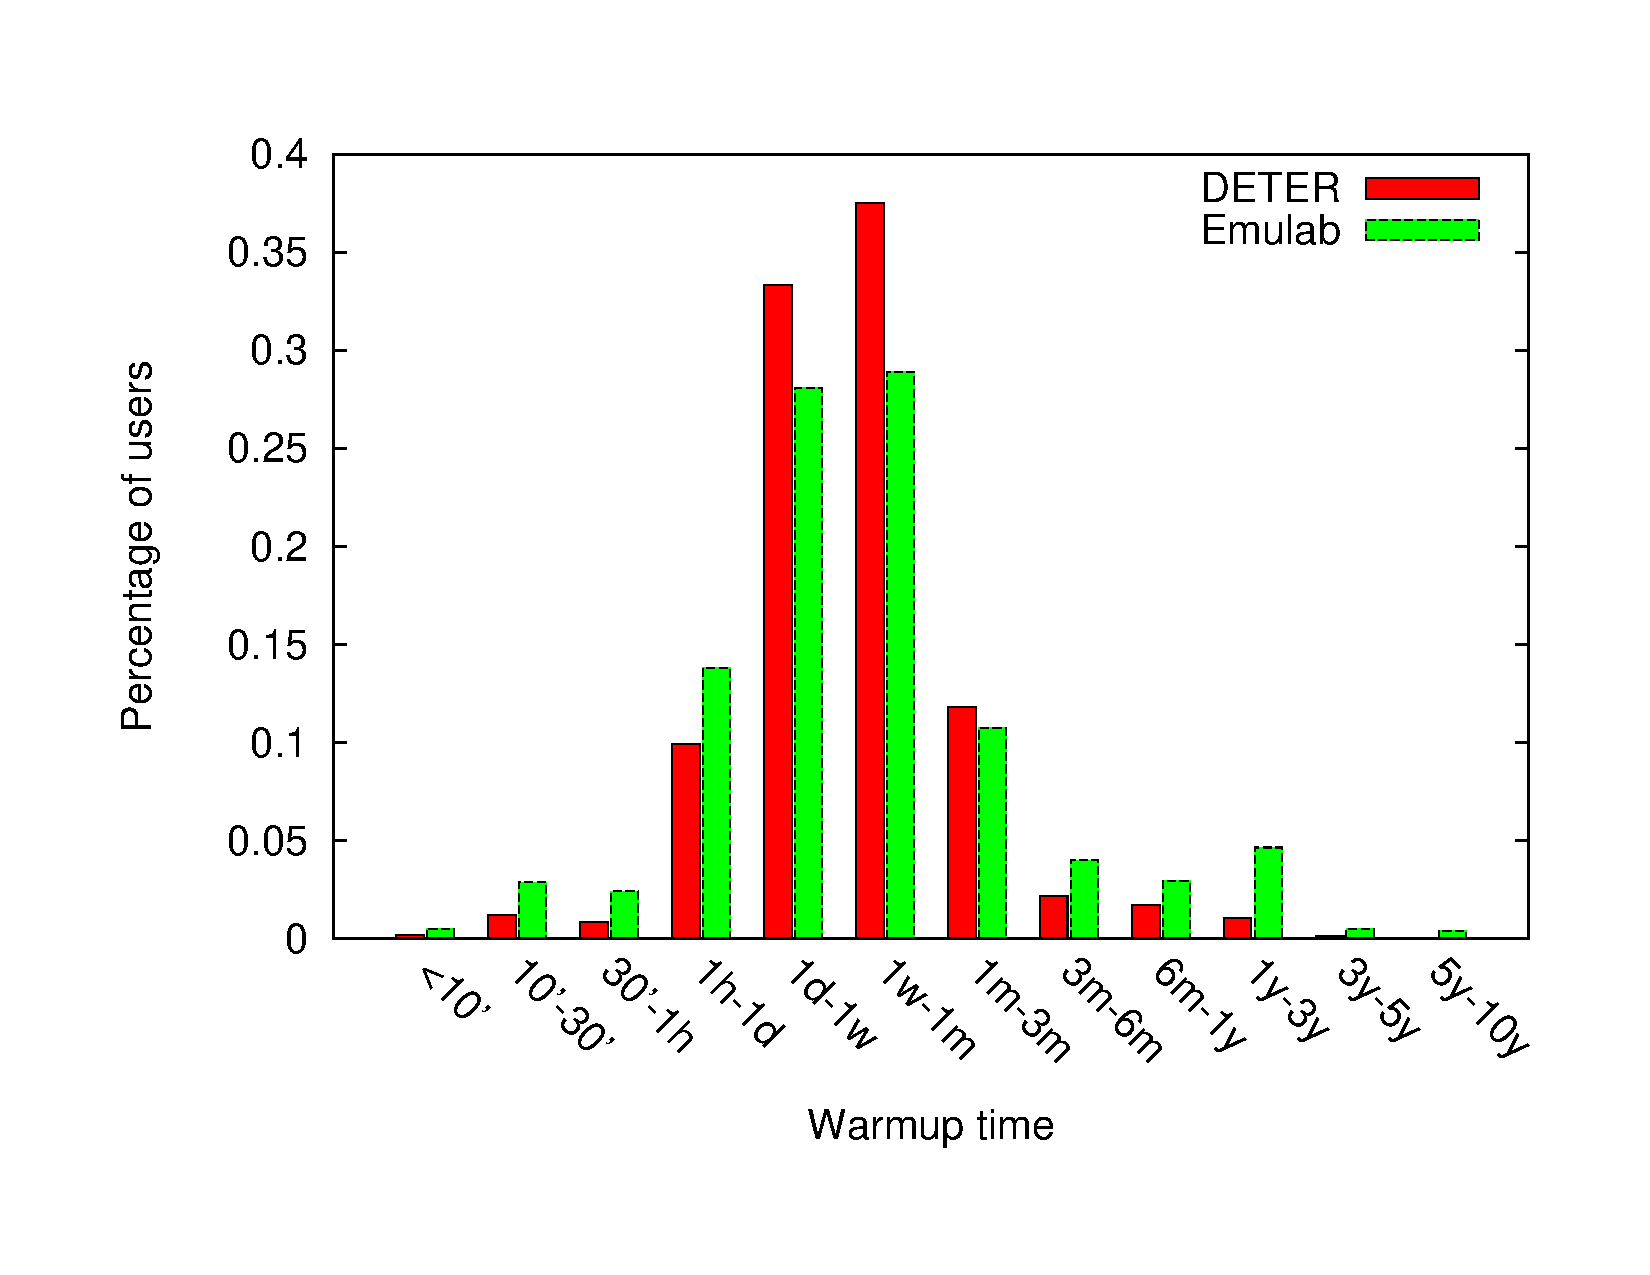
\includegraphics[width=3in]{figs/warmup_user.pdf} 
\caption{User warmup time in DETER and Emulab} 
\label{warmupus} \end{center} \end{figure}

\begin{figure}[htbp] \begin{center}
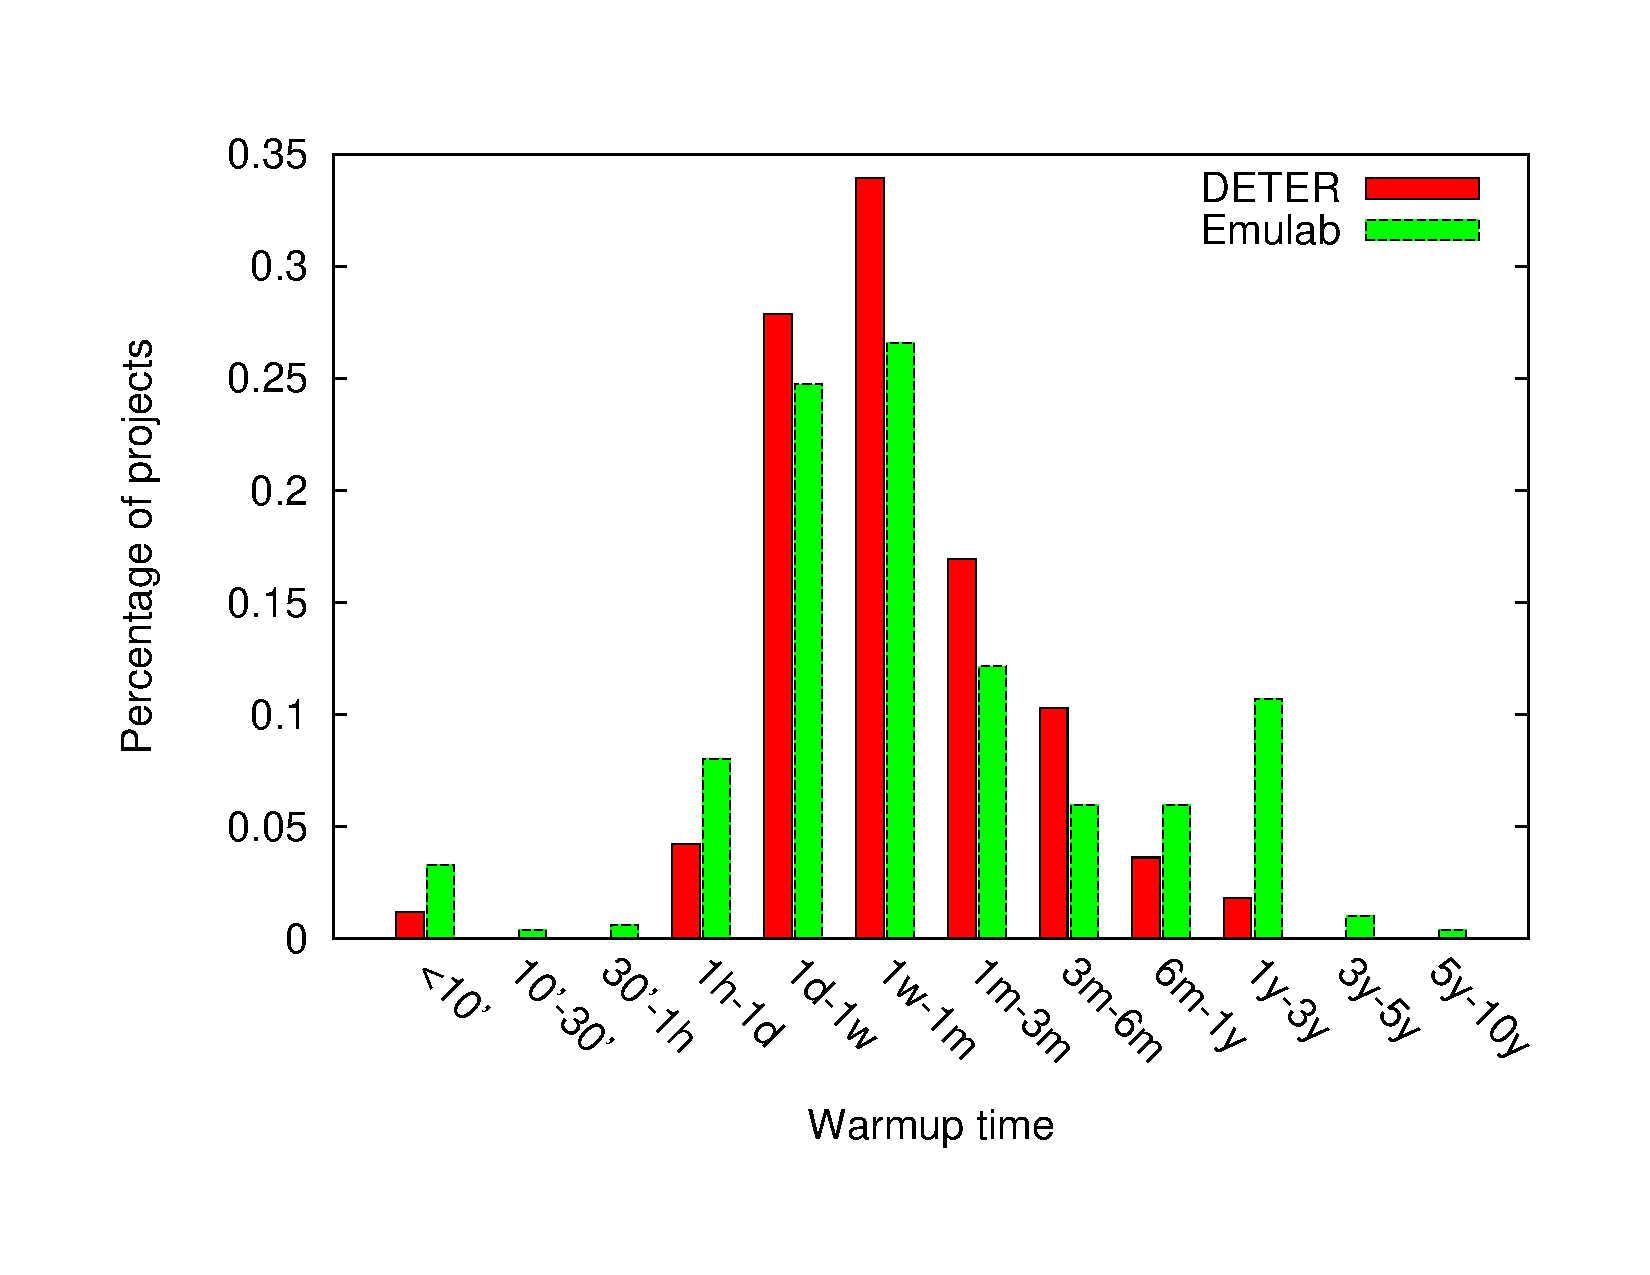
\includegraphics[width=3in]{figs/warmup_proj.pdf} 
\caption{Project warmup time in DETER and Emulab} \label{warmuppr} \end{center}
\end{figure}


\begin{figure}[htbp] \begin{center}
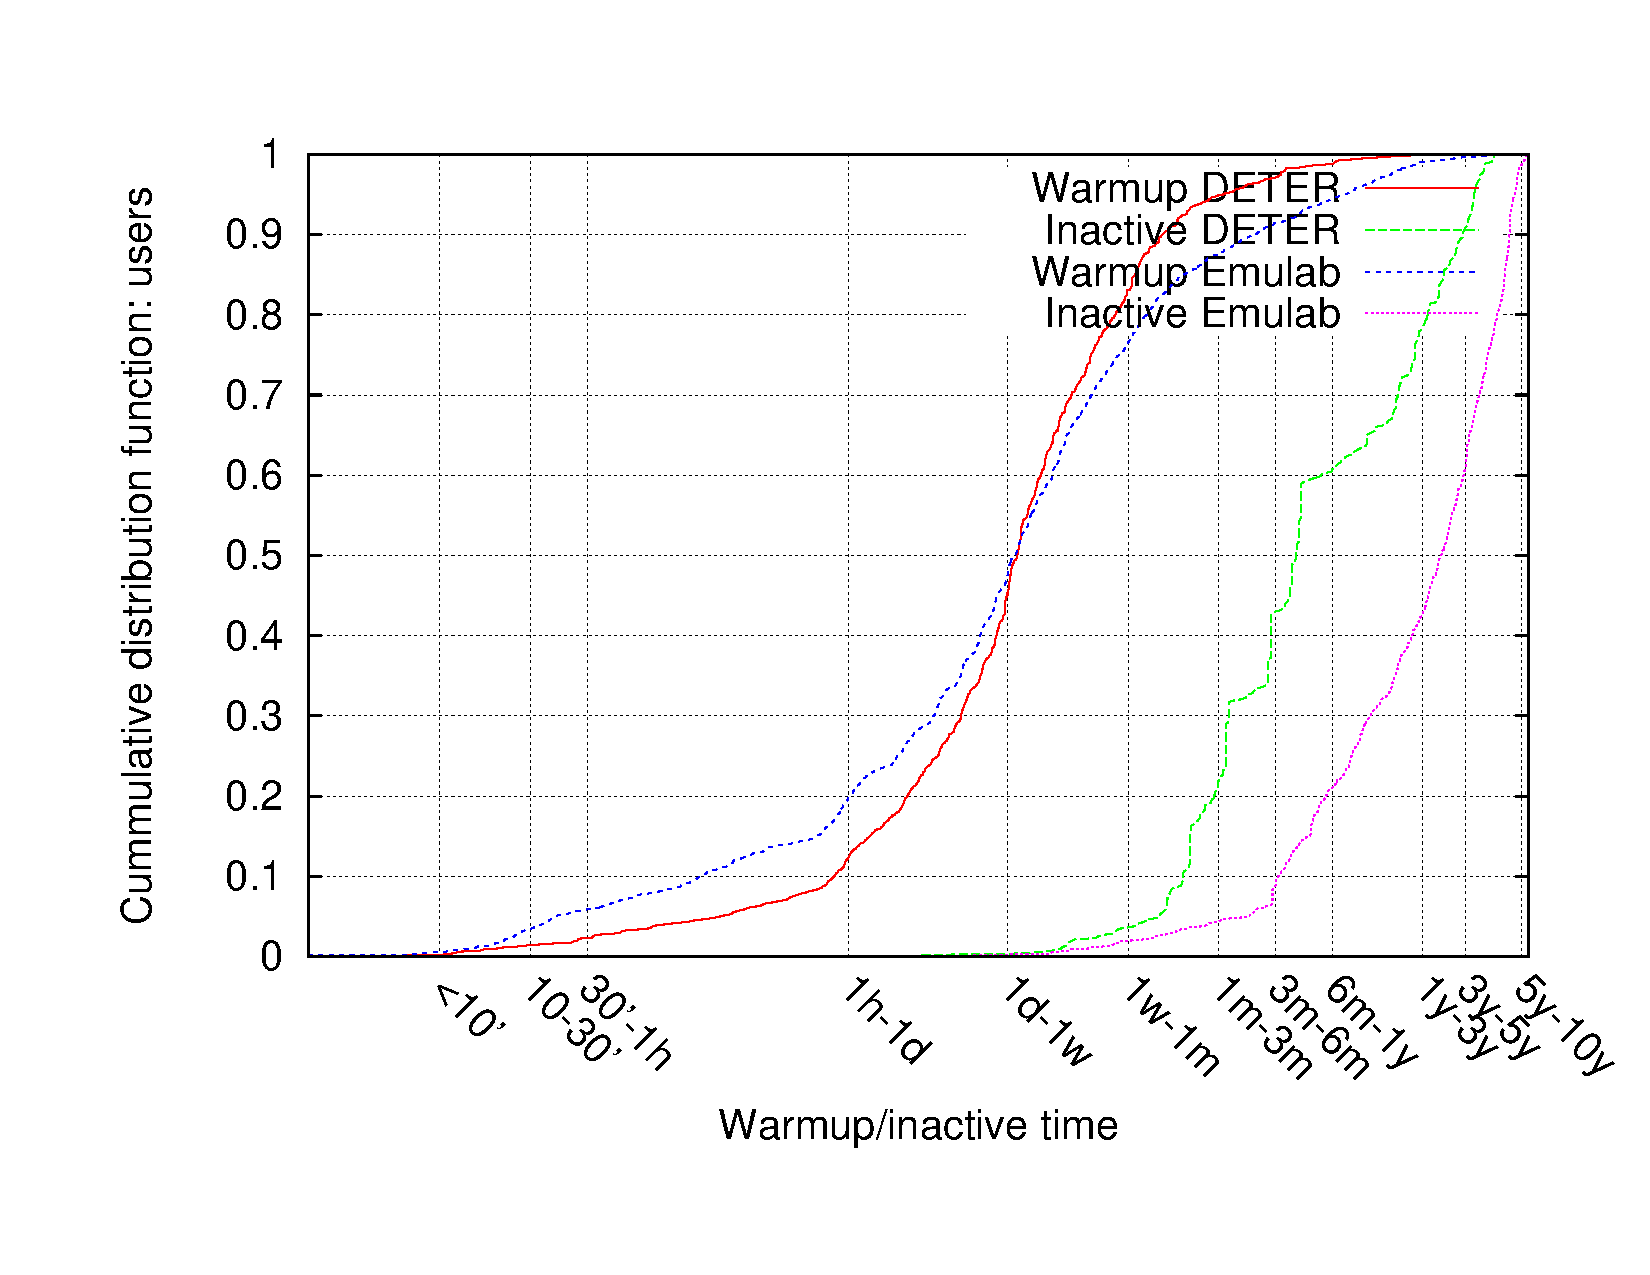
\includegraphics[width=3in]{figs/warmup_inact_user.pdf} 
\caption{User warmup and inactive time} \label{warmupinus} \end{center} \end{figure}


\begin{figure}[htbp] \begin{center}
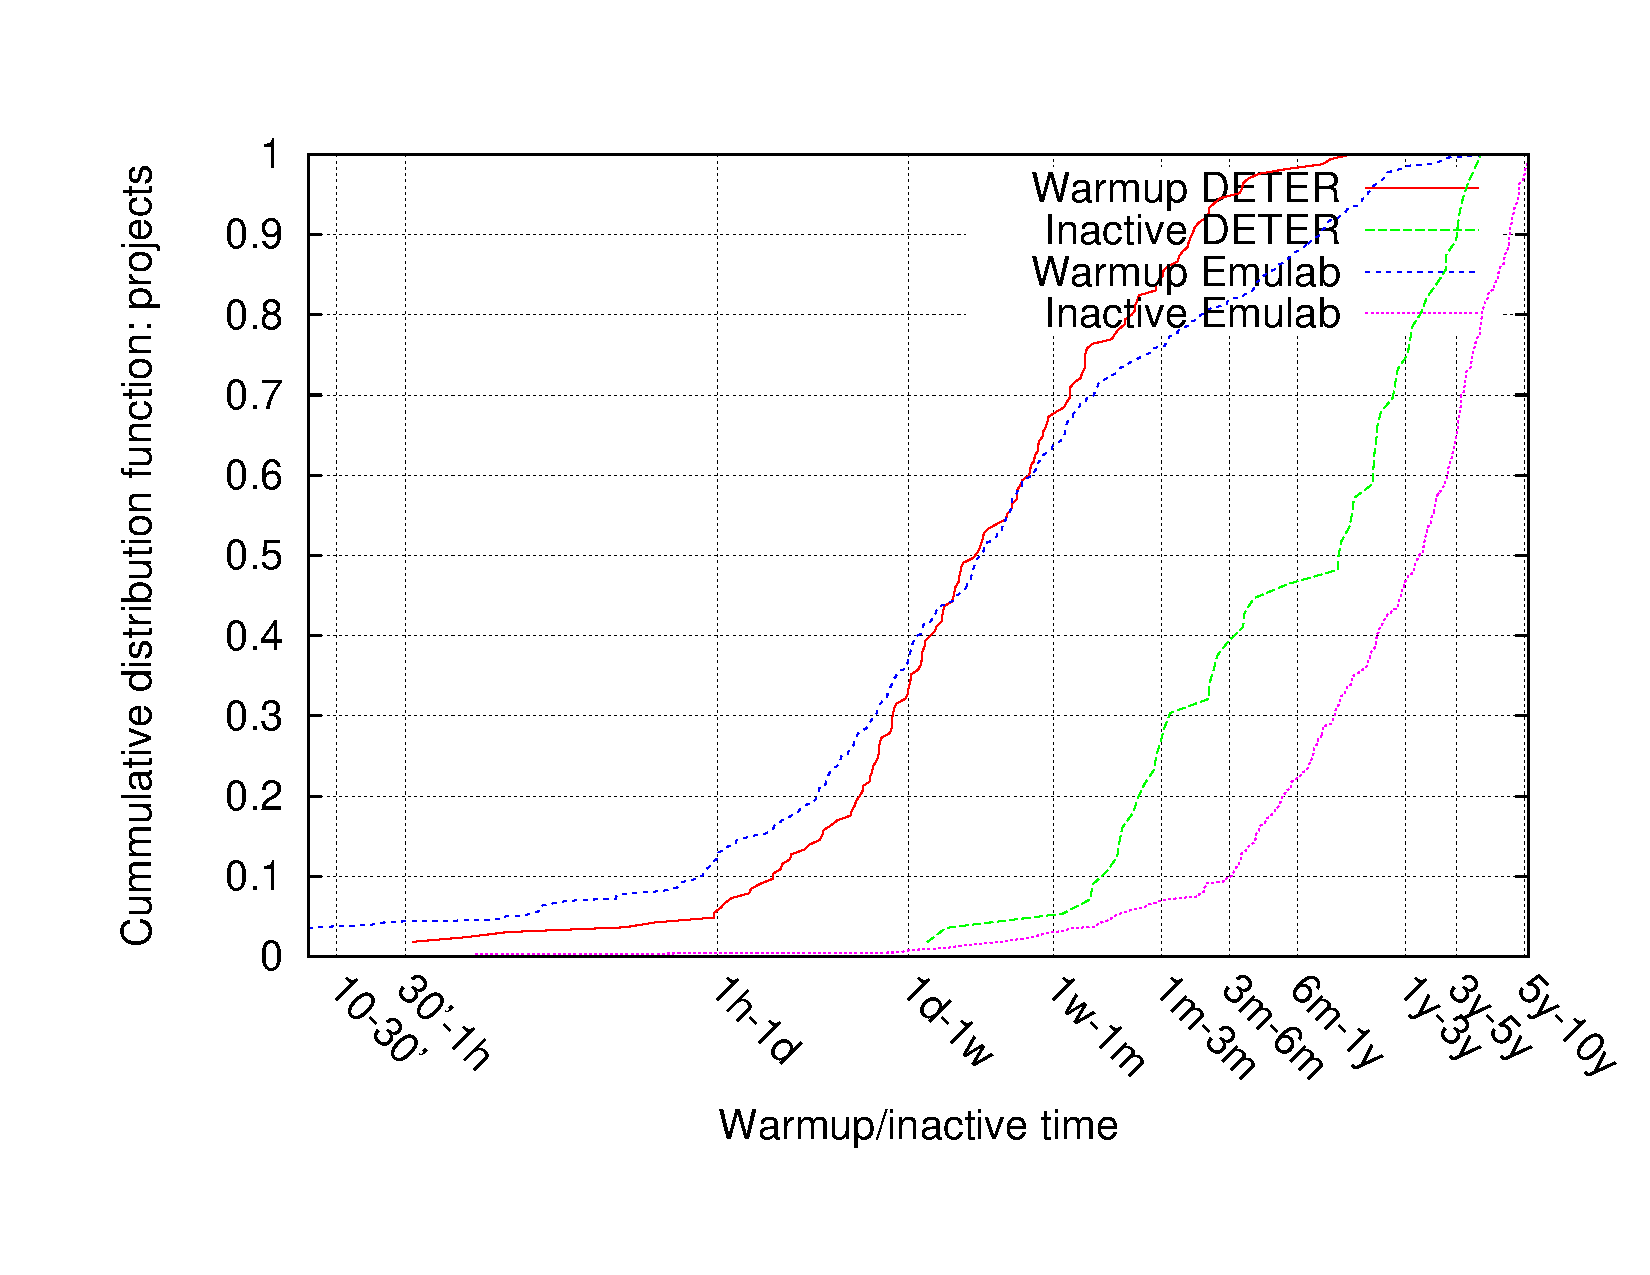
\includegraphics[width=3in]{figs/warmup_inact_proj.pdf} \caption{Project
warmup and inactive time} \label{warmupinpr} \end{center} \end{figure}

If we use the maximum value of the warmup time for the threshold then
the starred rows in the table \ref{cleaning} apply.

We now look at number of projects per research category. This is shown
in table \ref{projrc}. We took DDoS, worm and botnet out of attack
category because they are popular topics in recent years.

\begin{table}[htdp] \begin{center} \begin{tabular}{|c|c|} \hline
Research category & Projects \\\hline Attacks & 48  \\ DDoS & 18 \\
Architecture & 14\\ Infrastructure & 12 \\ Testbeds & 12 \\ Worms & 11
\\ Evaluation & 8 \\ Privacy & 6 \\ Botnets & 4 \\ \hline \end{tabular}
\end{center} \caption{Projects per research category} \label{projrc}
\end{table}%



Say exps from outcome projects follow same trends as all so we don't
show them here.

\begin{figure}[htbp] \begin{center}
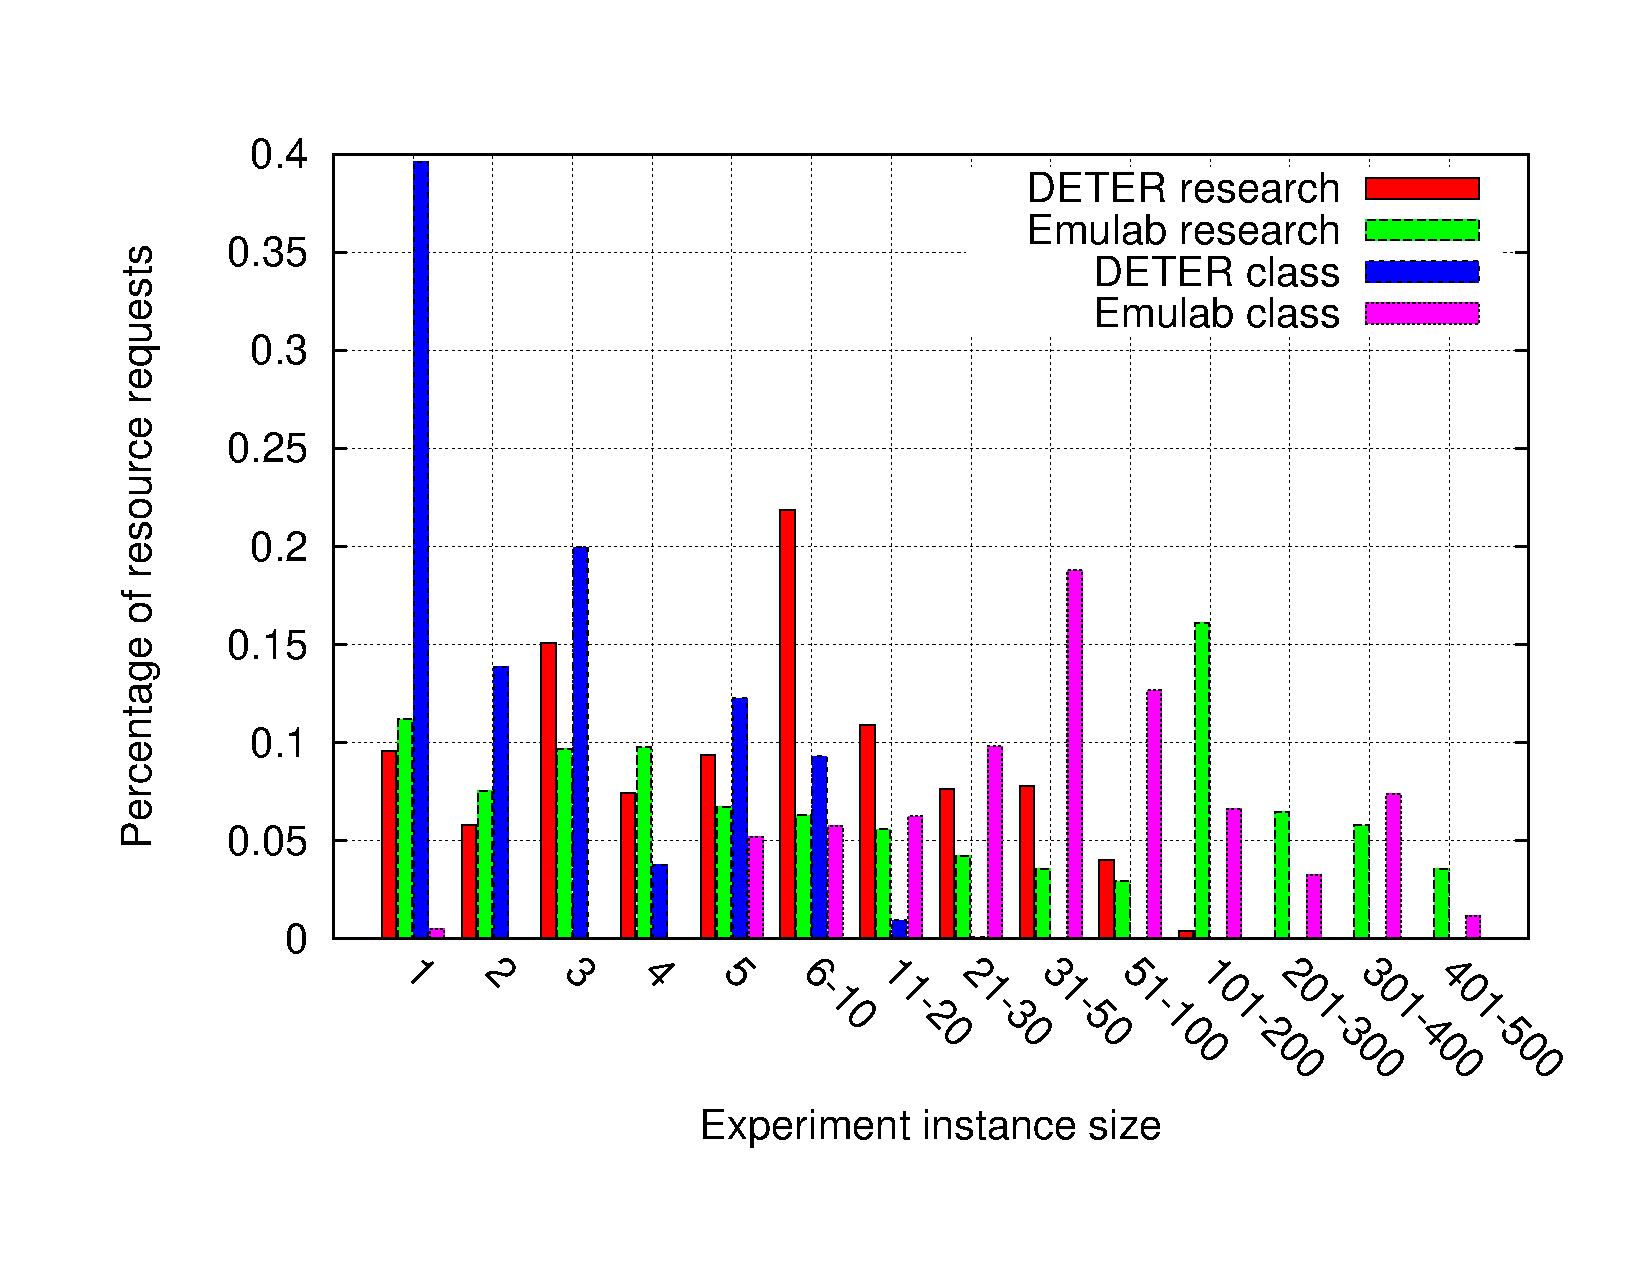
\includegraphics[width=3in,type=pdf,ext=.pdf,read=.pdf]
{figs/exp.size.gnu} \caption{Experiment instance size} \label{expsize} \end{center}
\end{figure}

\begin{figure}[htbp] \begin{center}
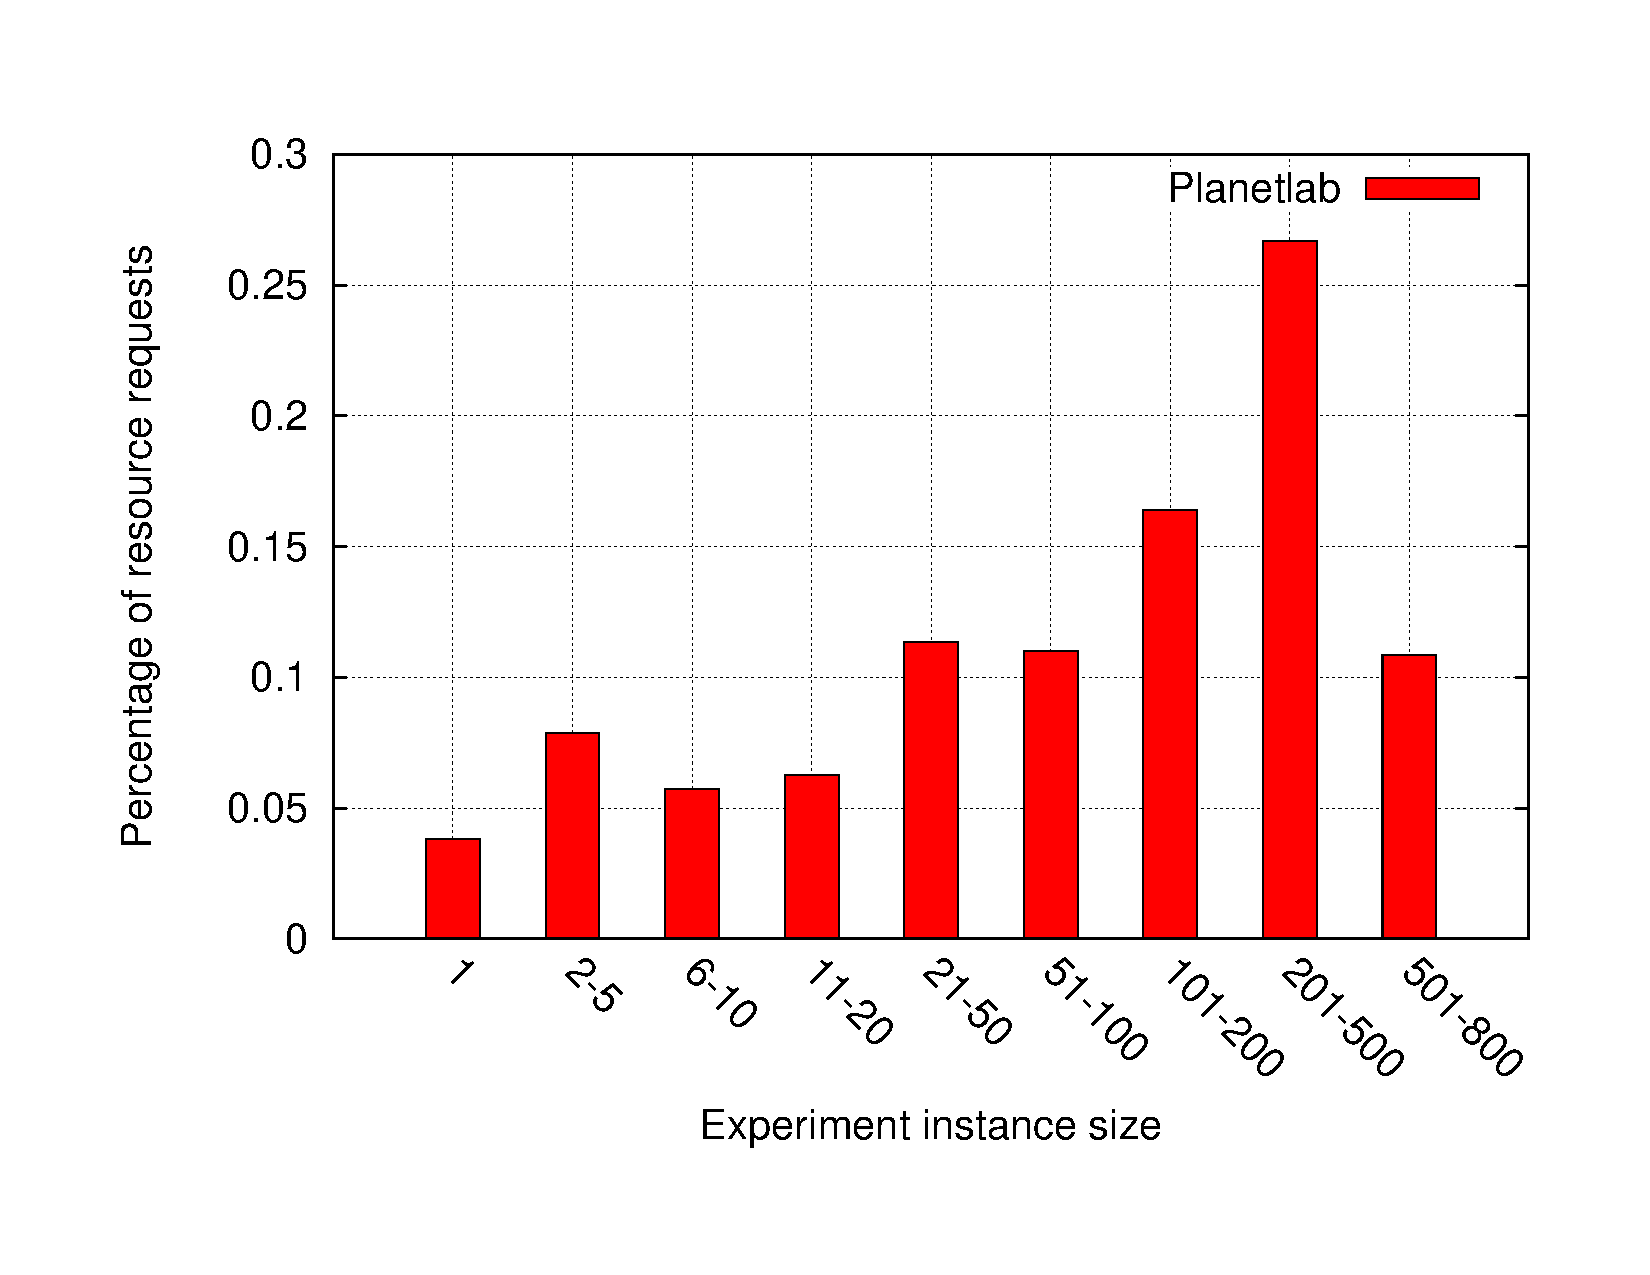
\includegraphics[width=3in,type=pdf,ext=.pdf,read=.pdf]
{figs/planet.size.gnu} \caption{Experiment instance size in Planetlab} \label{expsize}
\end{center} \end{figure}

\begin{figure}[htbp] \begin{center} 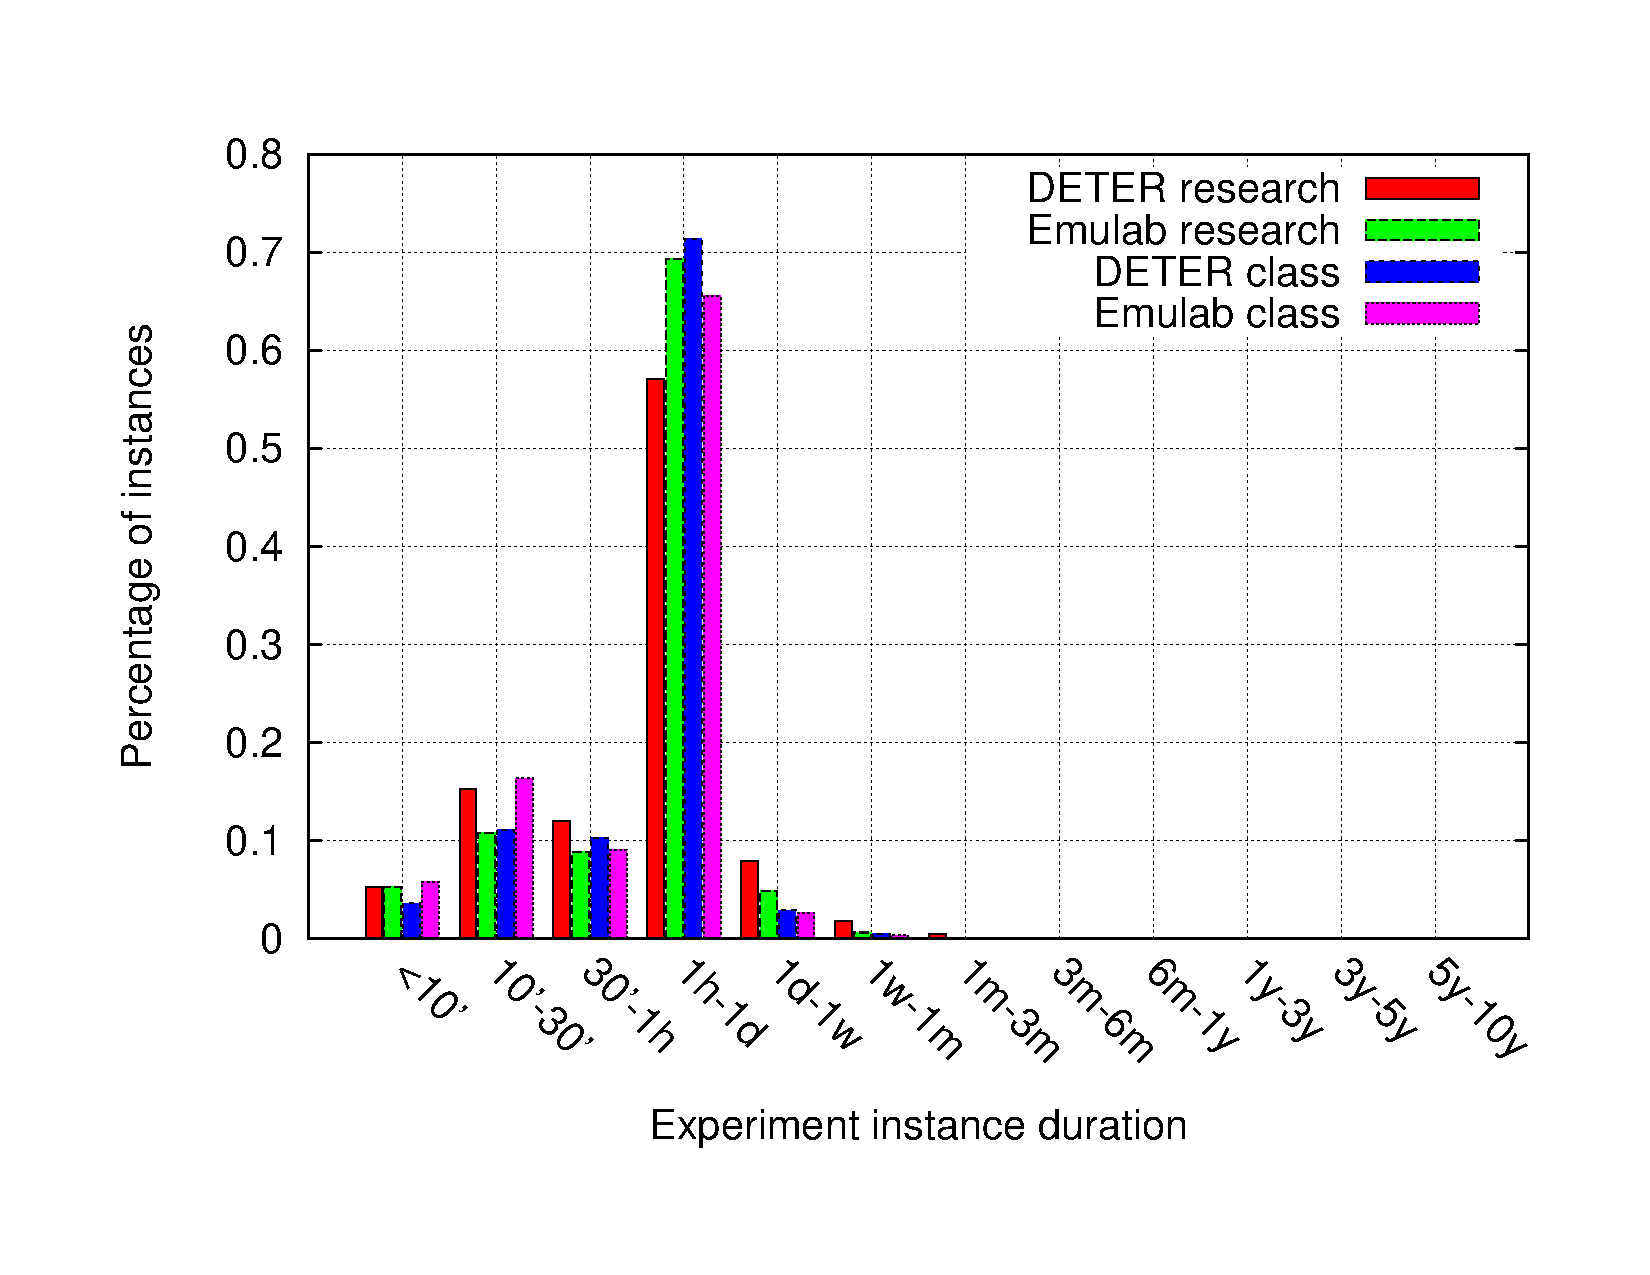
\includegraphics[width=3in,
type=pdf,ext=.pdf,read=.pdf]{figs/exp.dur.gnu} \caption{Experiment
instance duration} \label{expdur} \end{center} \end{figure}

\begin{figure}[htbp] \begin{center} 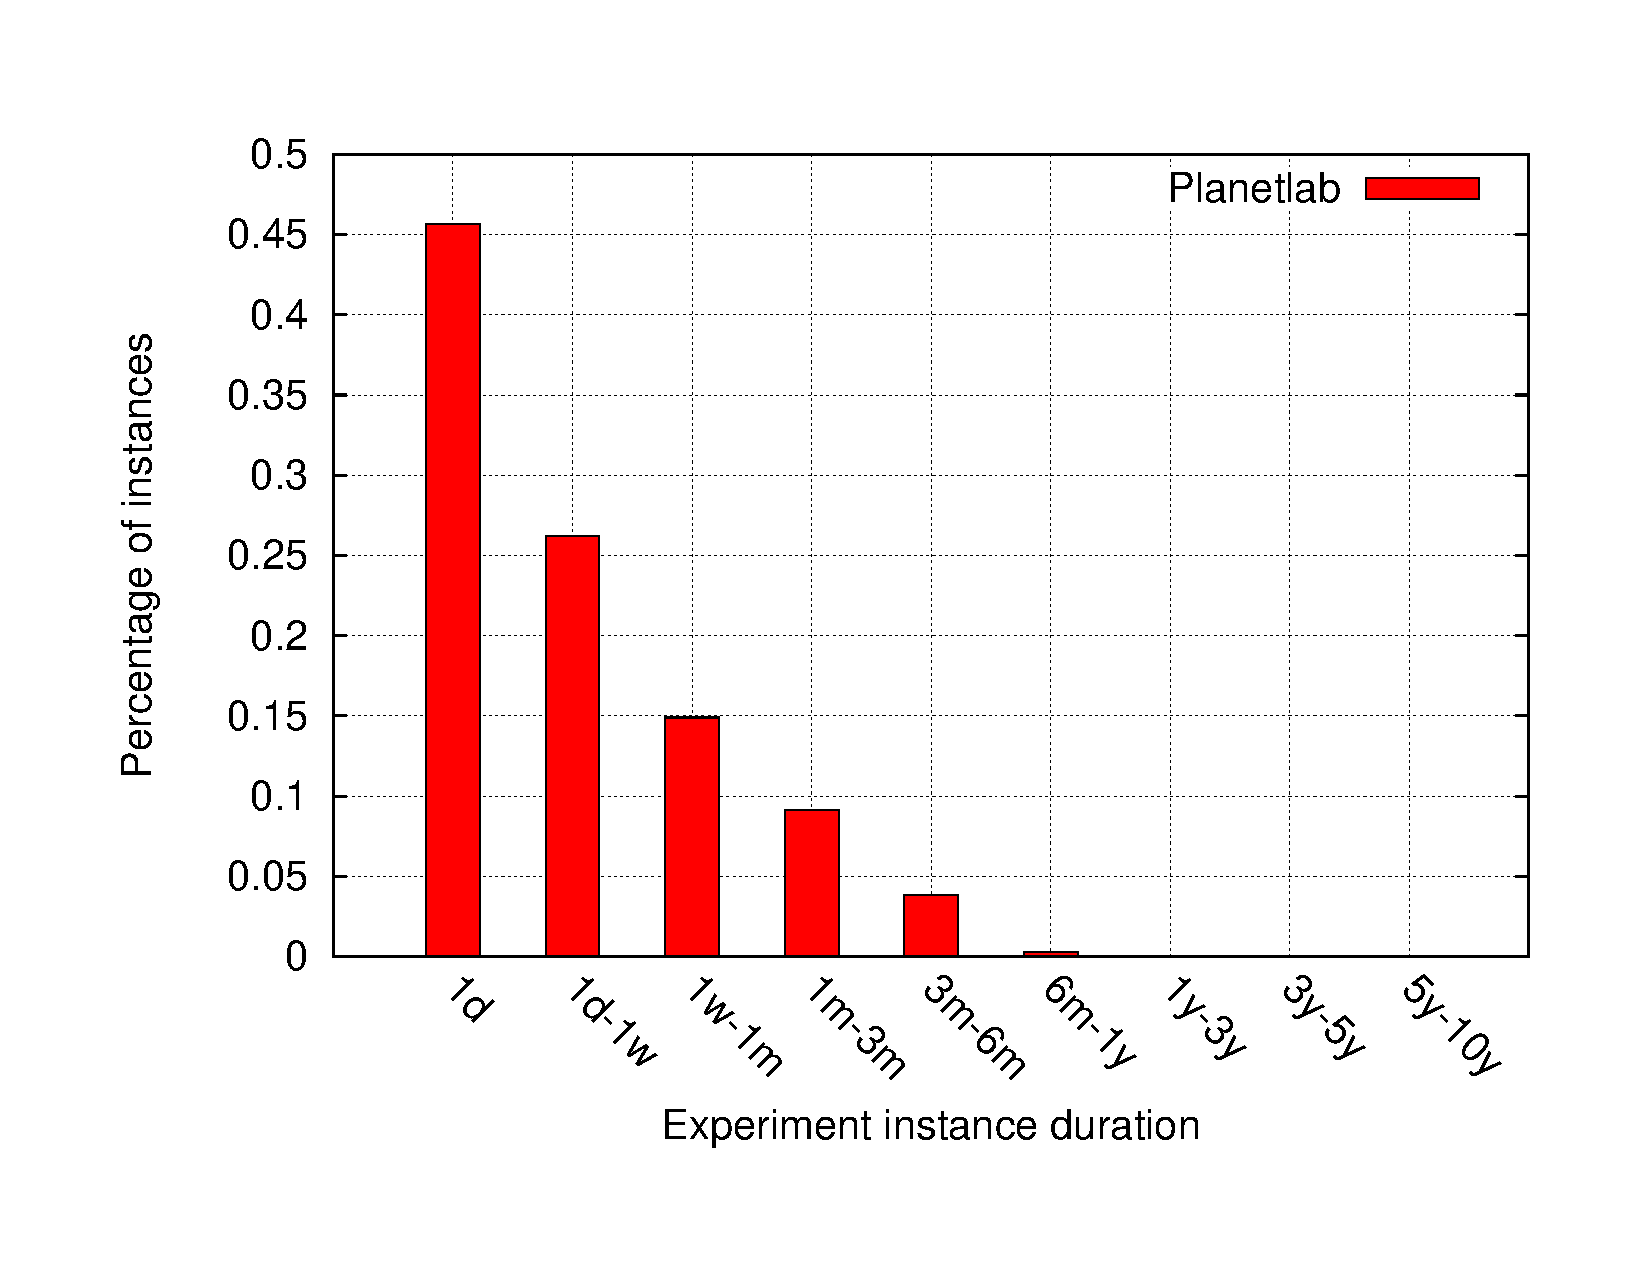
\includegraphics[width=3in,
type=pdf,ext=.pdf,read=.pdf]{figs/planet.dur.gnu} \caption{Experiment
instance duration in Planetlab} \label{expdur} \end{center} \end{figure}

\begin{figure}[htbp] \begin{center} 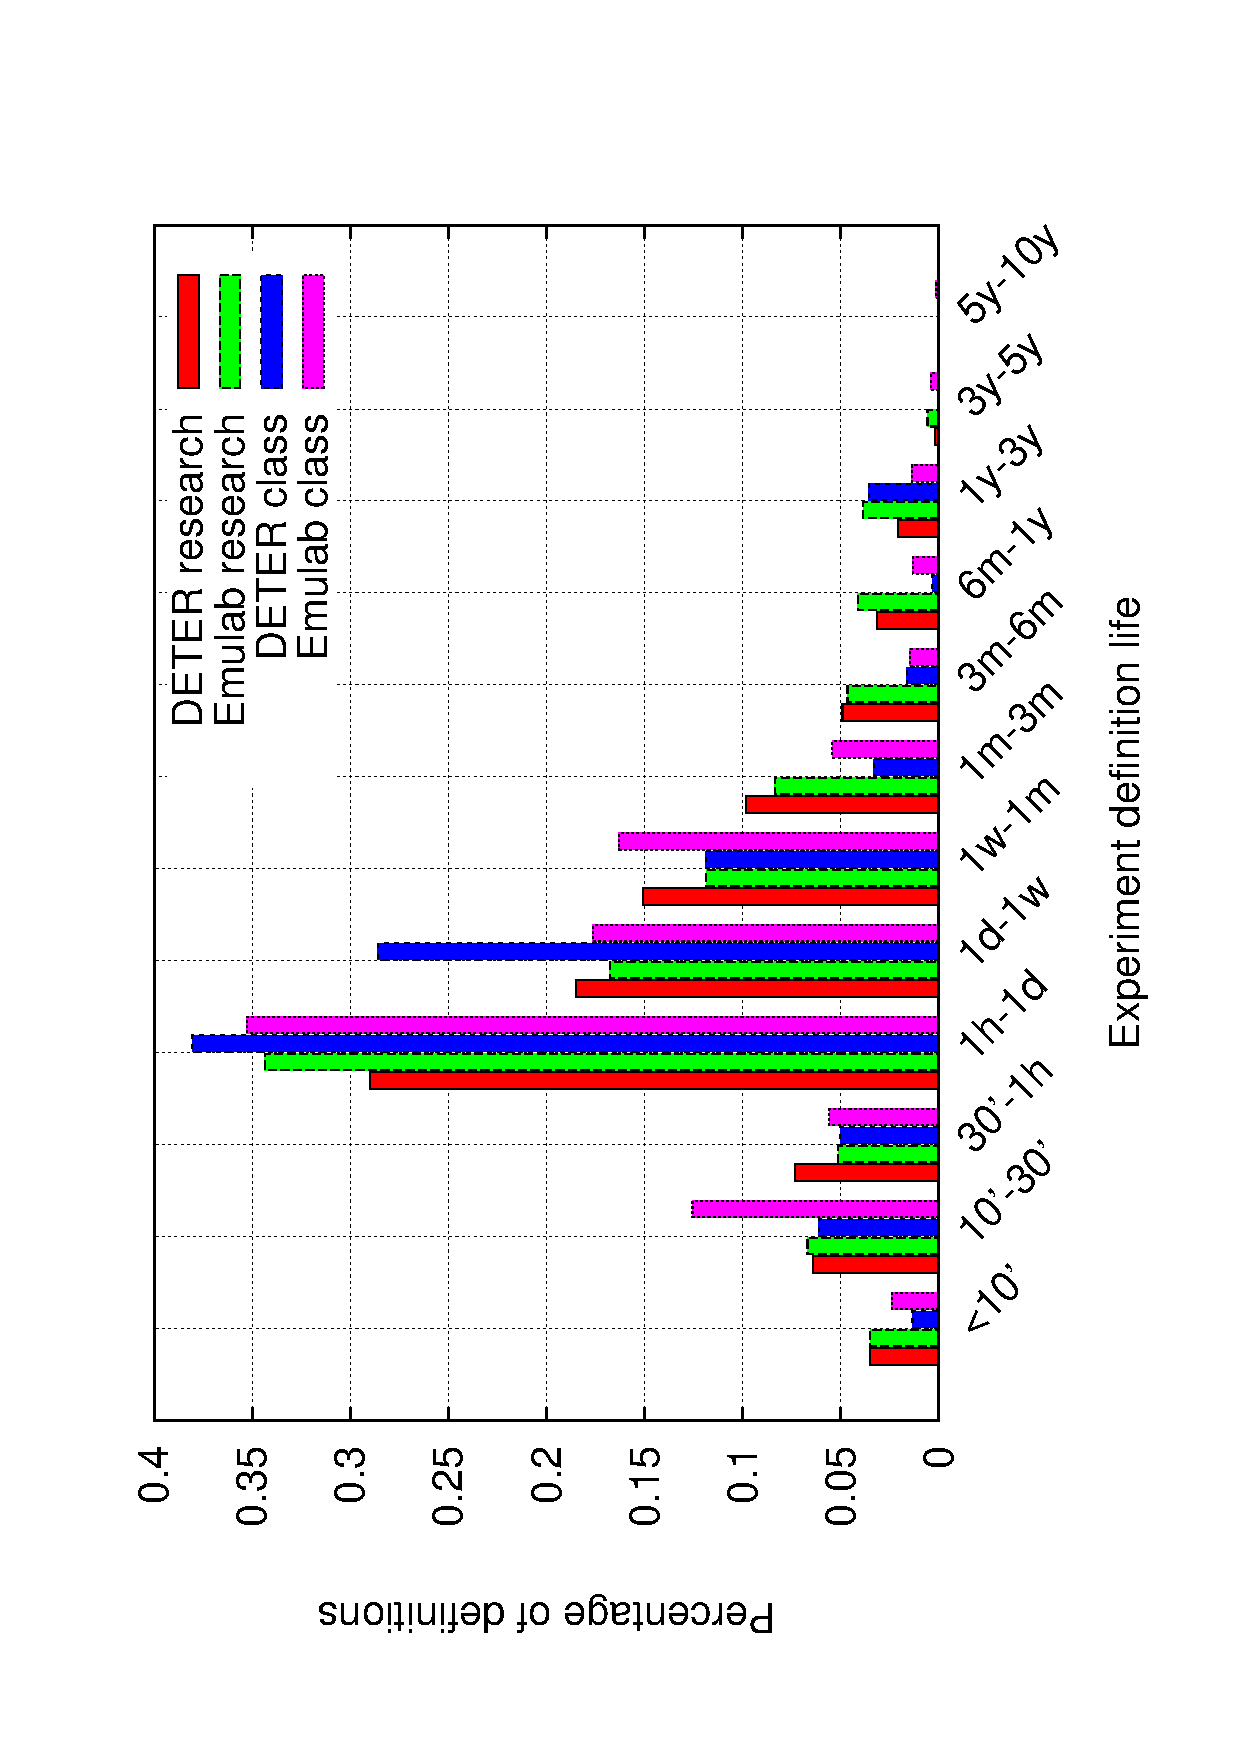
\includegraphics[width=3in,
type=pdf,ext=.pdf,read=.pdf]{figs/exp.life.gnu} \caption{Experiment
definition life} \label{explife} \end{center} \end{figure}

\begin{figure}[htbp] \begin{center} 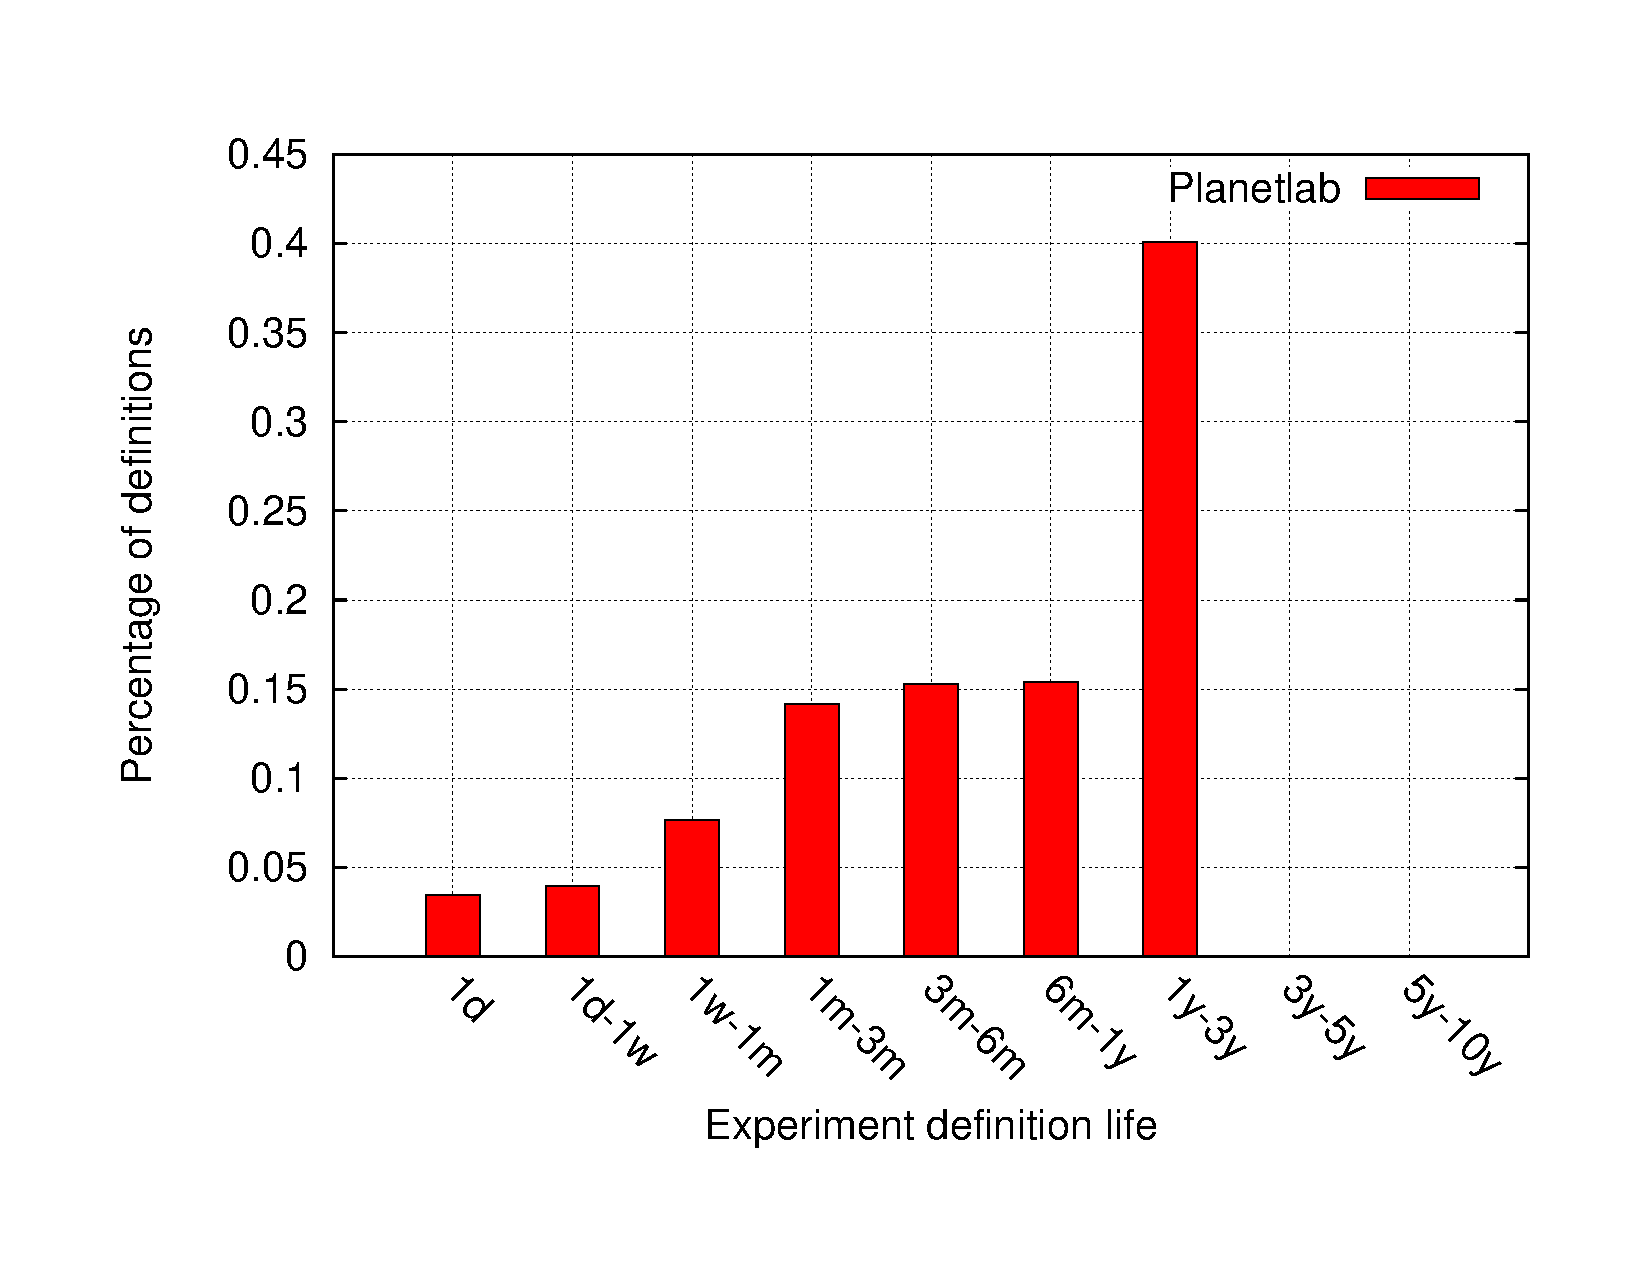
\includegraphics[width=3in,
type=pdf,ext=.pdf,read=.pdf]{figs/planet.life.gnu} \caption{Experiment
definition life in Planetlab} \label{explife} \end{center} \end{figure}

\begin{figure}[htbp] \begin{center} 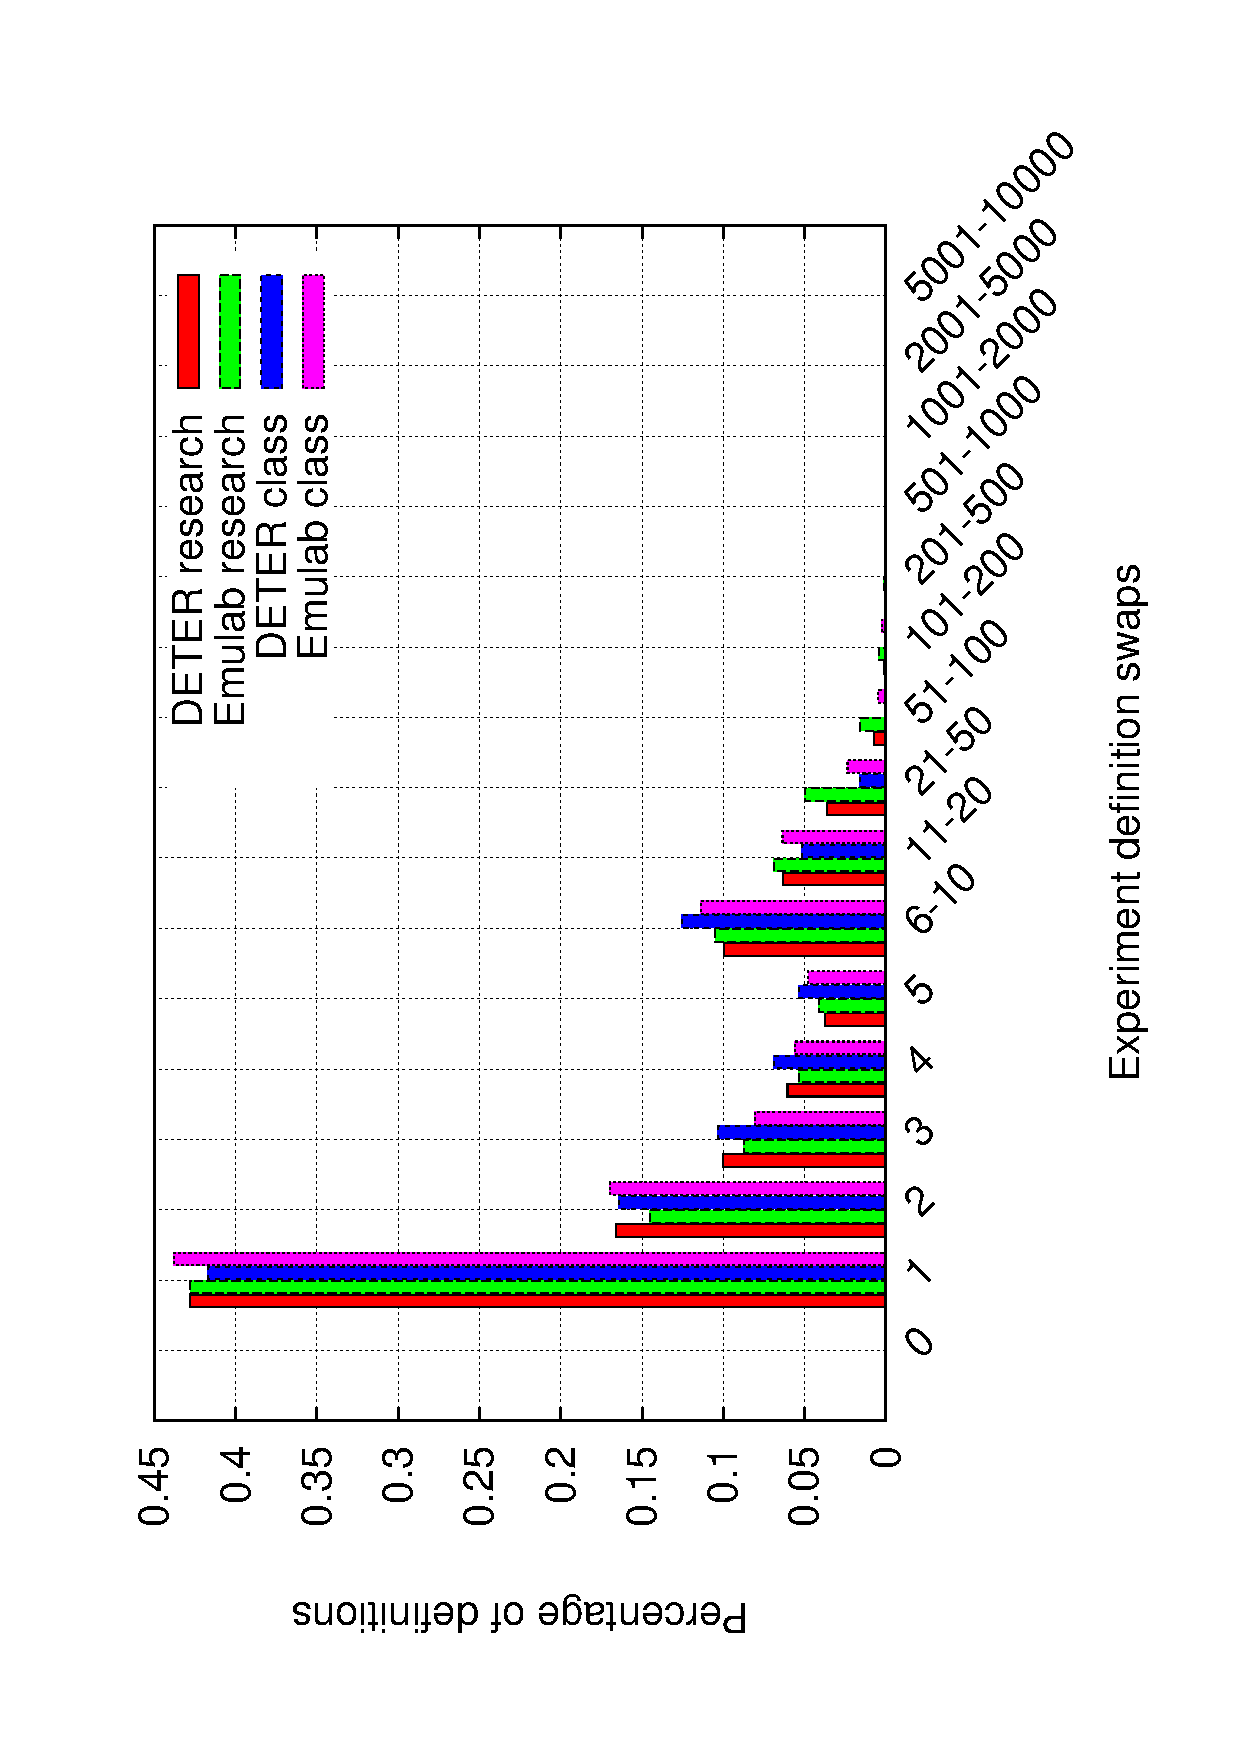
\includegraphics[width=3in,
type=pdf,ext=.pdf,read=.pdf]{figs/exp.swaps.gnu} \caption{Experiment
definition swaps} \label{expswaps} \end{center} \end{figure}

\begin{figure}[htbp] \begin{center} 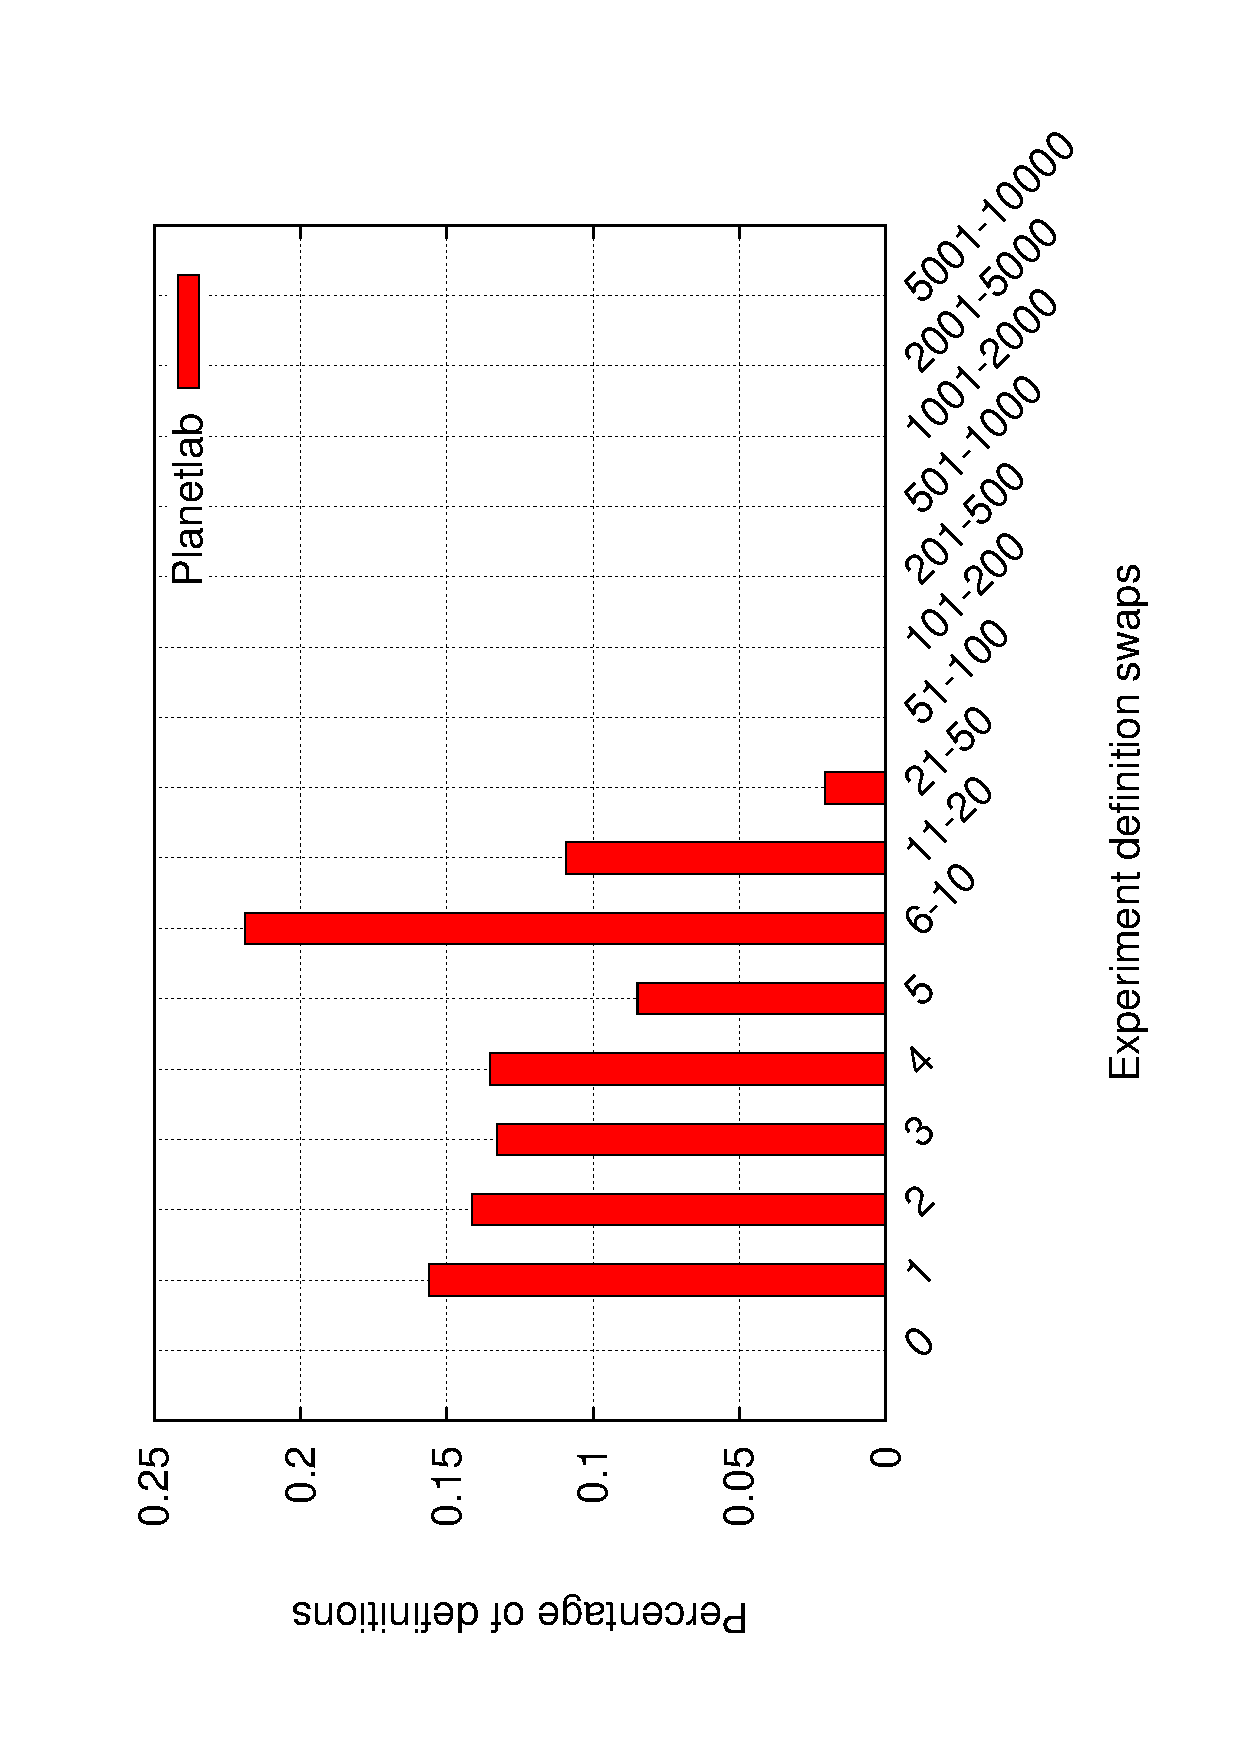
\includegraphics[width=3in,
type=pdf,ext=.pdf,read=.pdf]{figs/planet.swaps.gnu} \caption{Experiment
definition swaps in Planetlab} \label{expswaps} \end{center}
\end{figure}

\begin{figure*}[htbp] \begin{center} 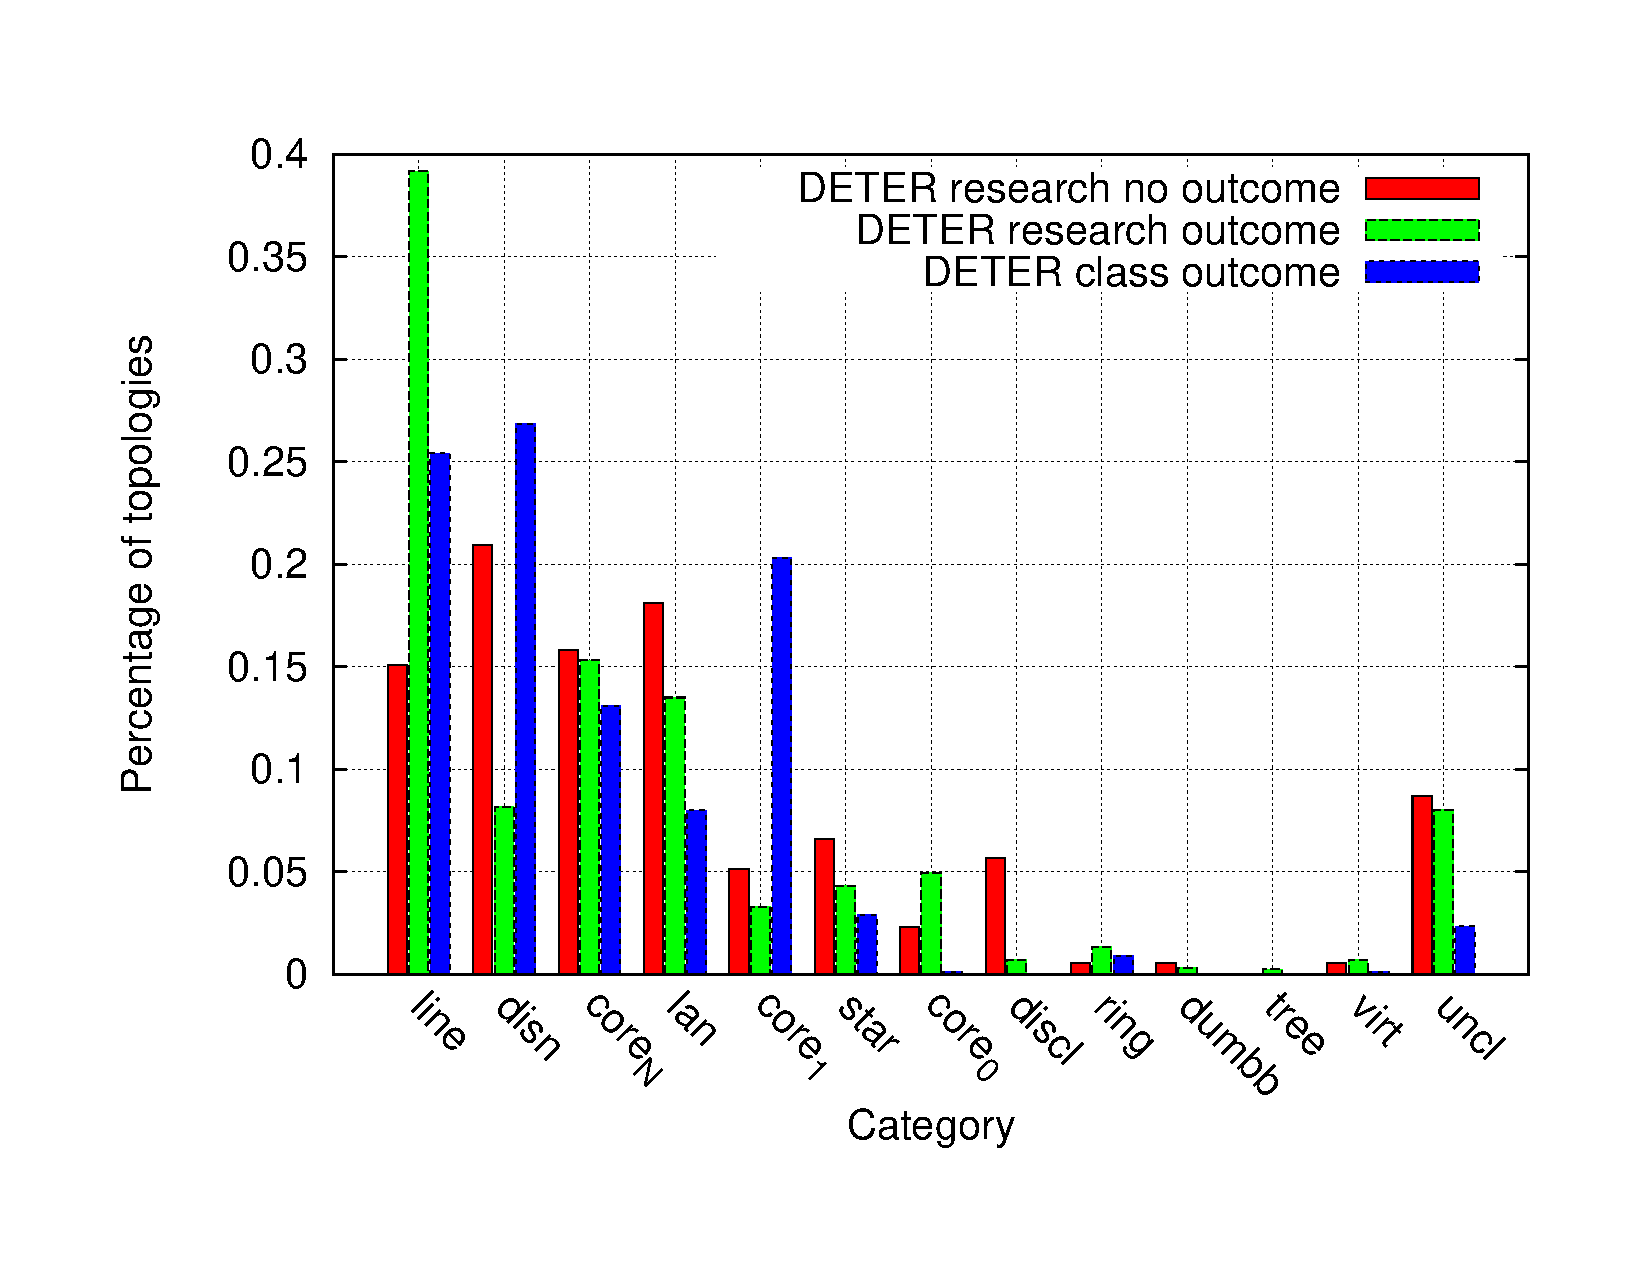
\includegraphics[width=3in,
type=pdf,ext=.pdf,read=.pdf]{figs/topo.gnu} 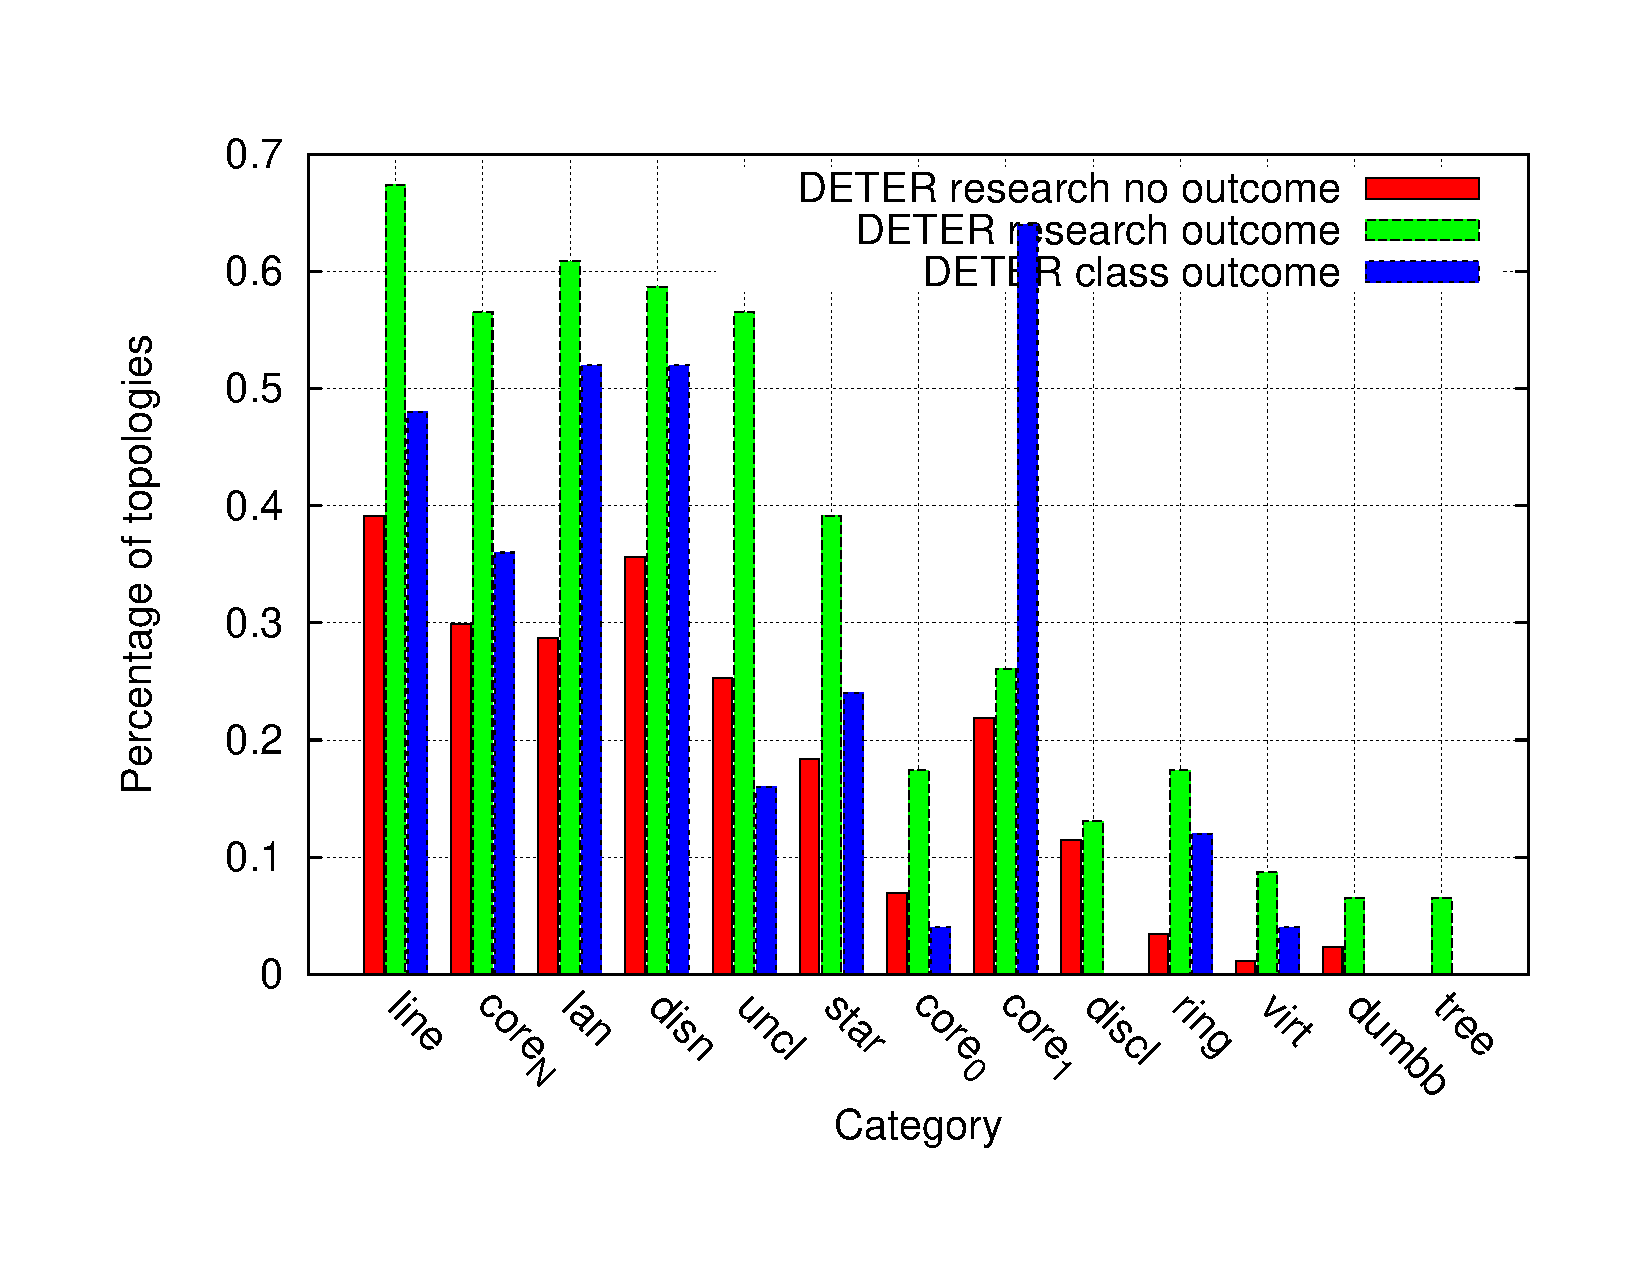
\includegraphics[width=3in,
type=pdf,ext=.pdf,read=.pdf]{figs/topop.gnu} \caption{Experiment
topologies in DETER: experiment vs project distribution} \label{topo}
\end{center} \end{figure*}



\subsection{Project Distributions} 

In this case trends differ between all and outcome projects. Those with
outcome are definitely more active. \begin{figure*}[htbp] \begin{center}
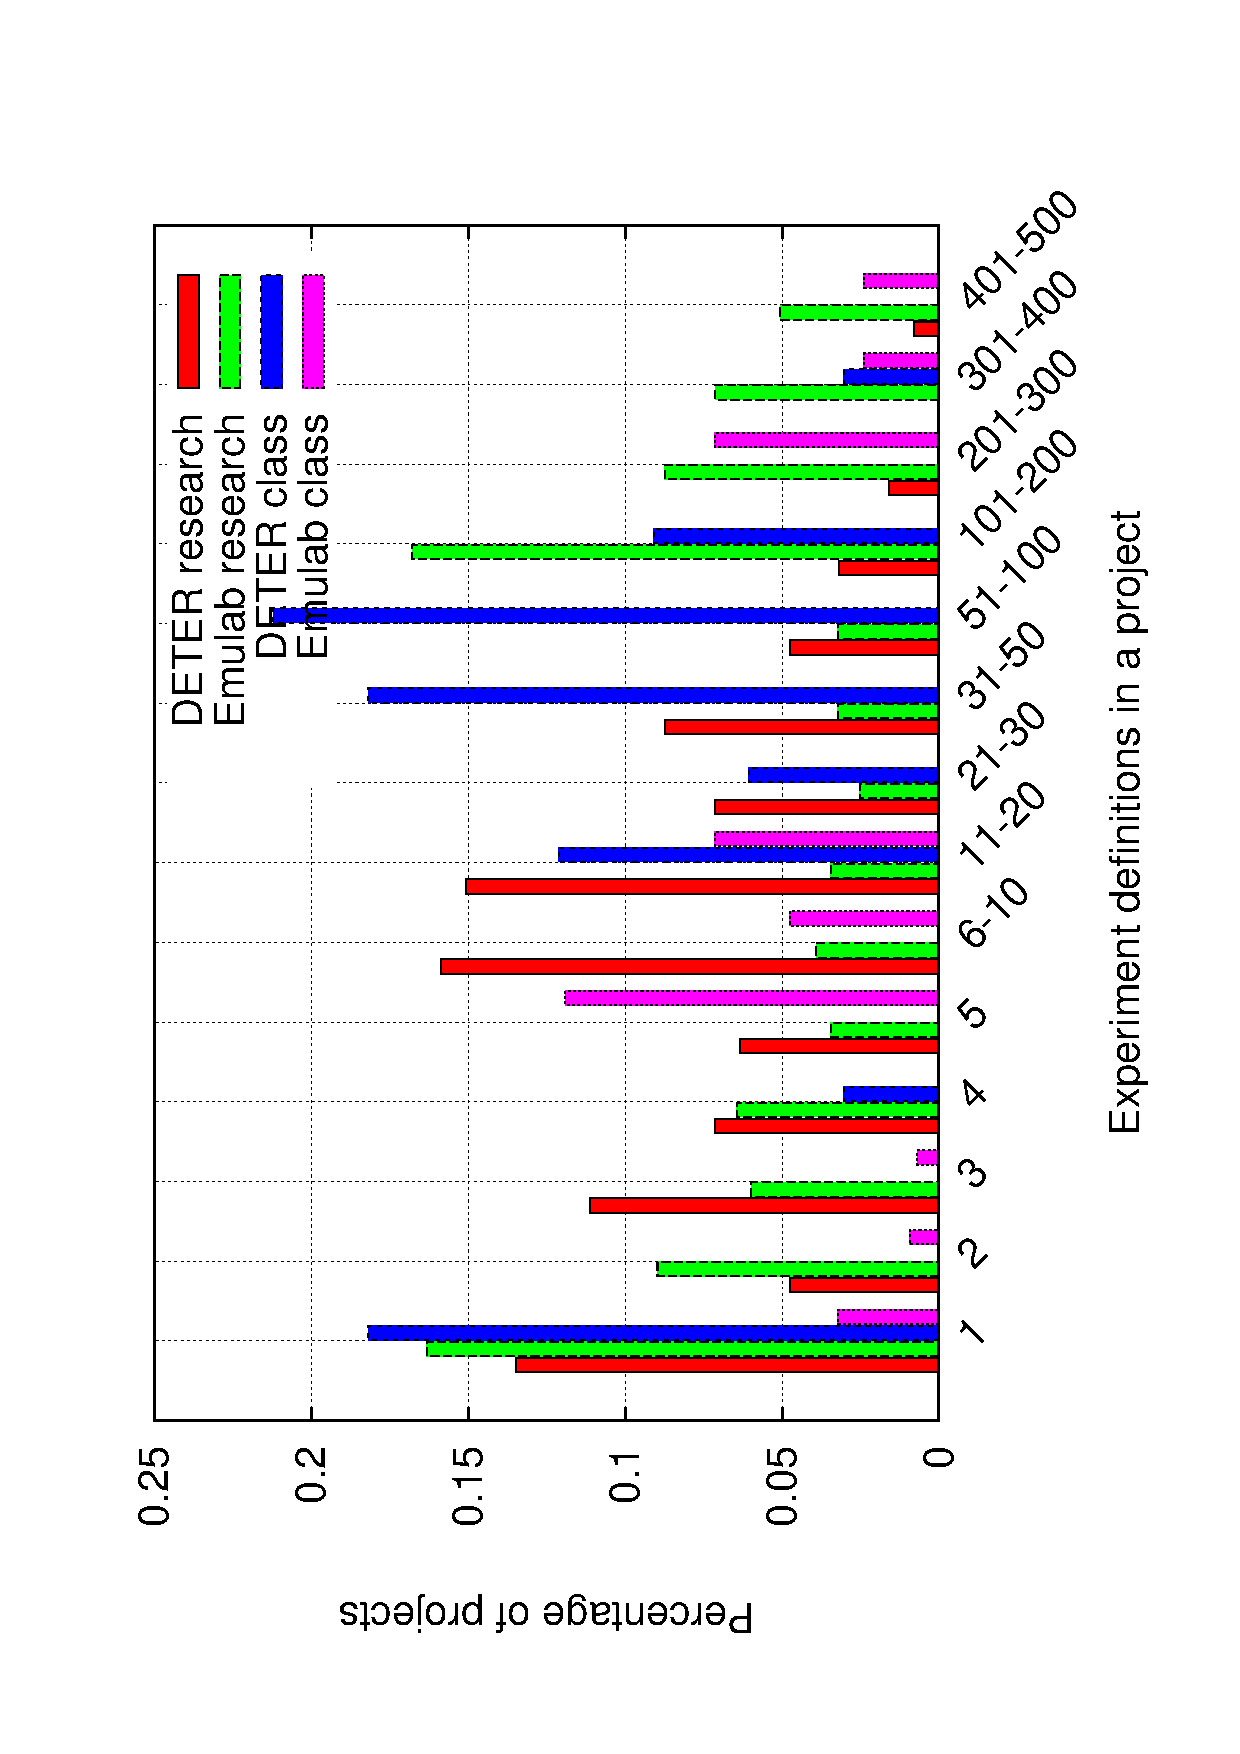
\includegraphics[width=3in,
type=pdf,ext=.pdf,read=.pdf]{figs/proj.size.gnu}
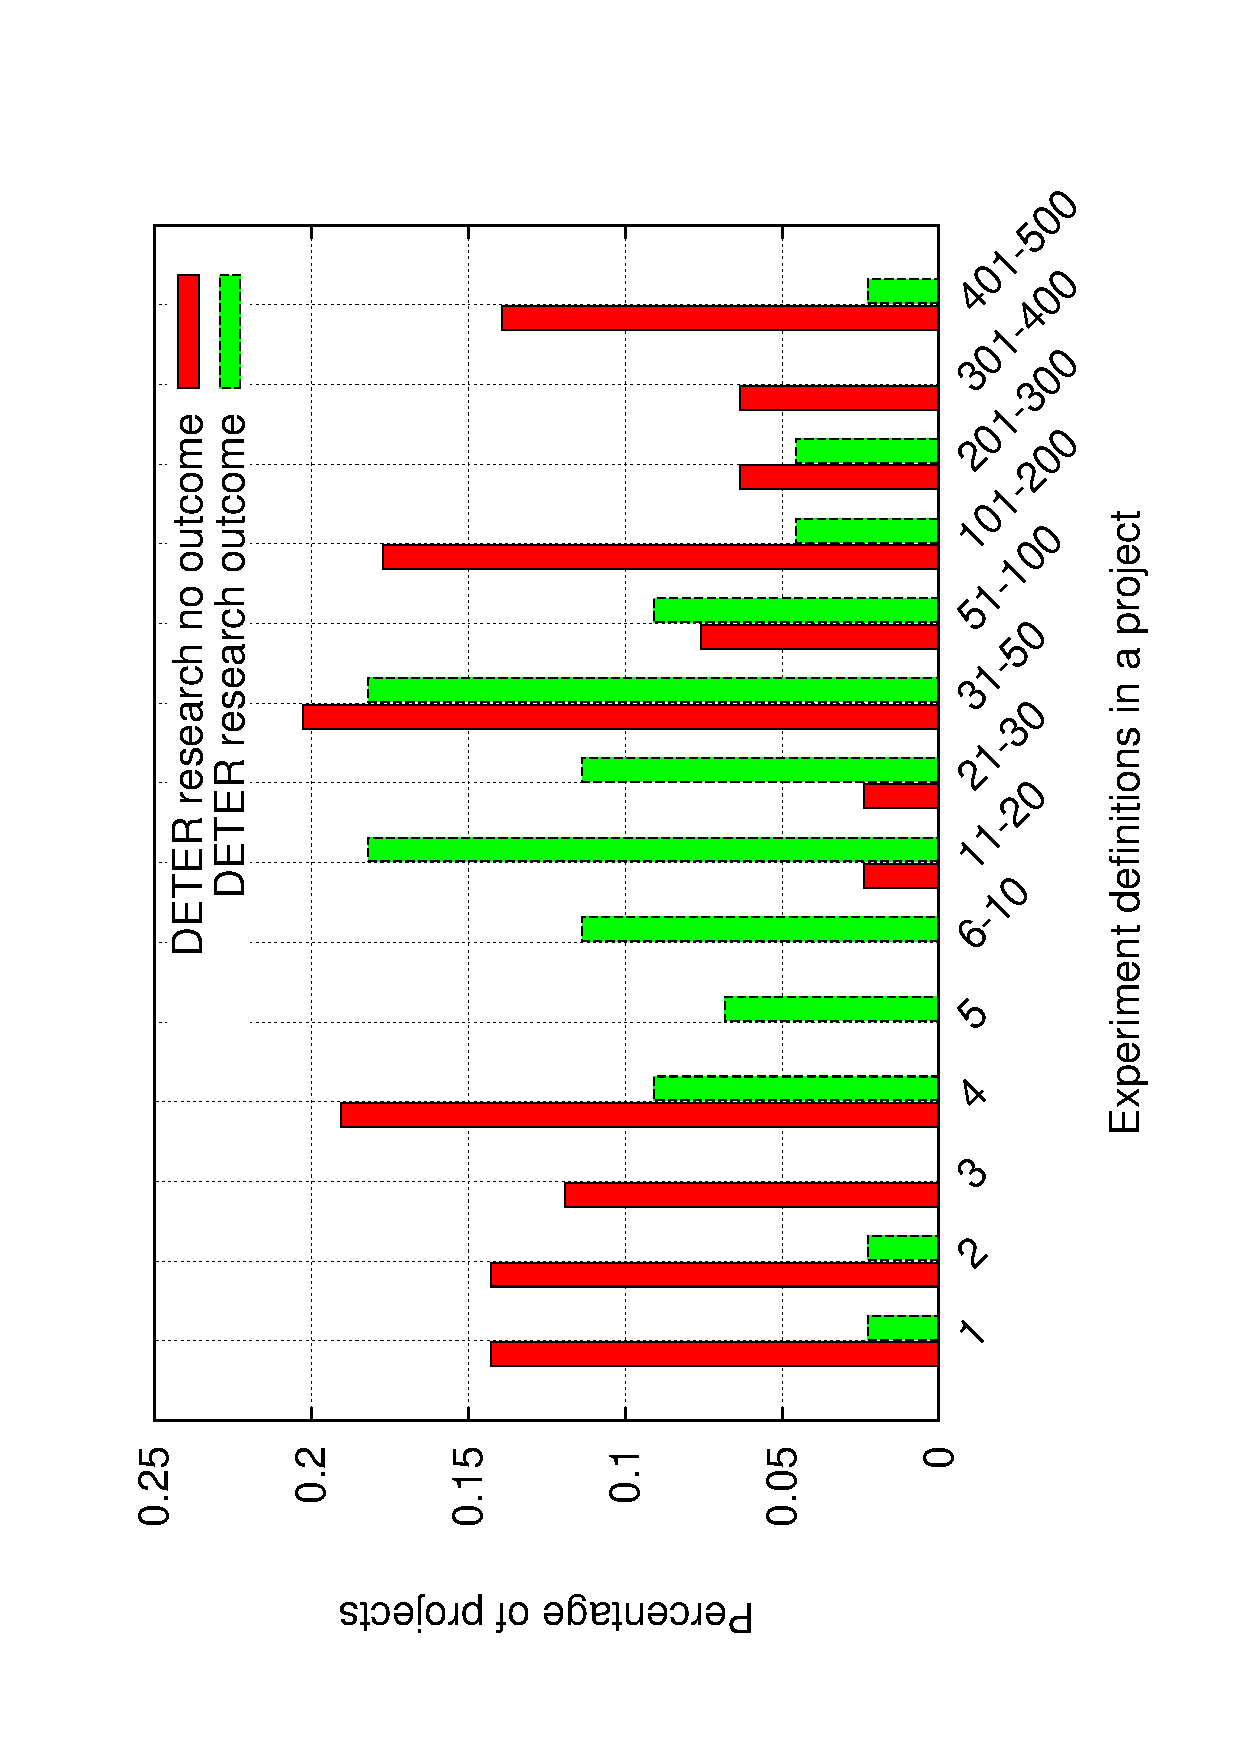
\includegraphics[width=3in,
type=pdf,ext=.pdf,read=.pdf]{figs/proj.size.cmp.gnu}
\caption{Experiments per project. Left: DETER vs Emulab, Right: All vs
outcome} \label{projsize} \end{center} \end{figure*}

\begin{figure*}[htbp] \begin{center} 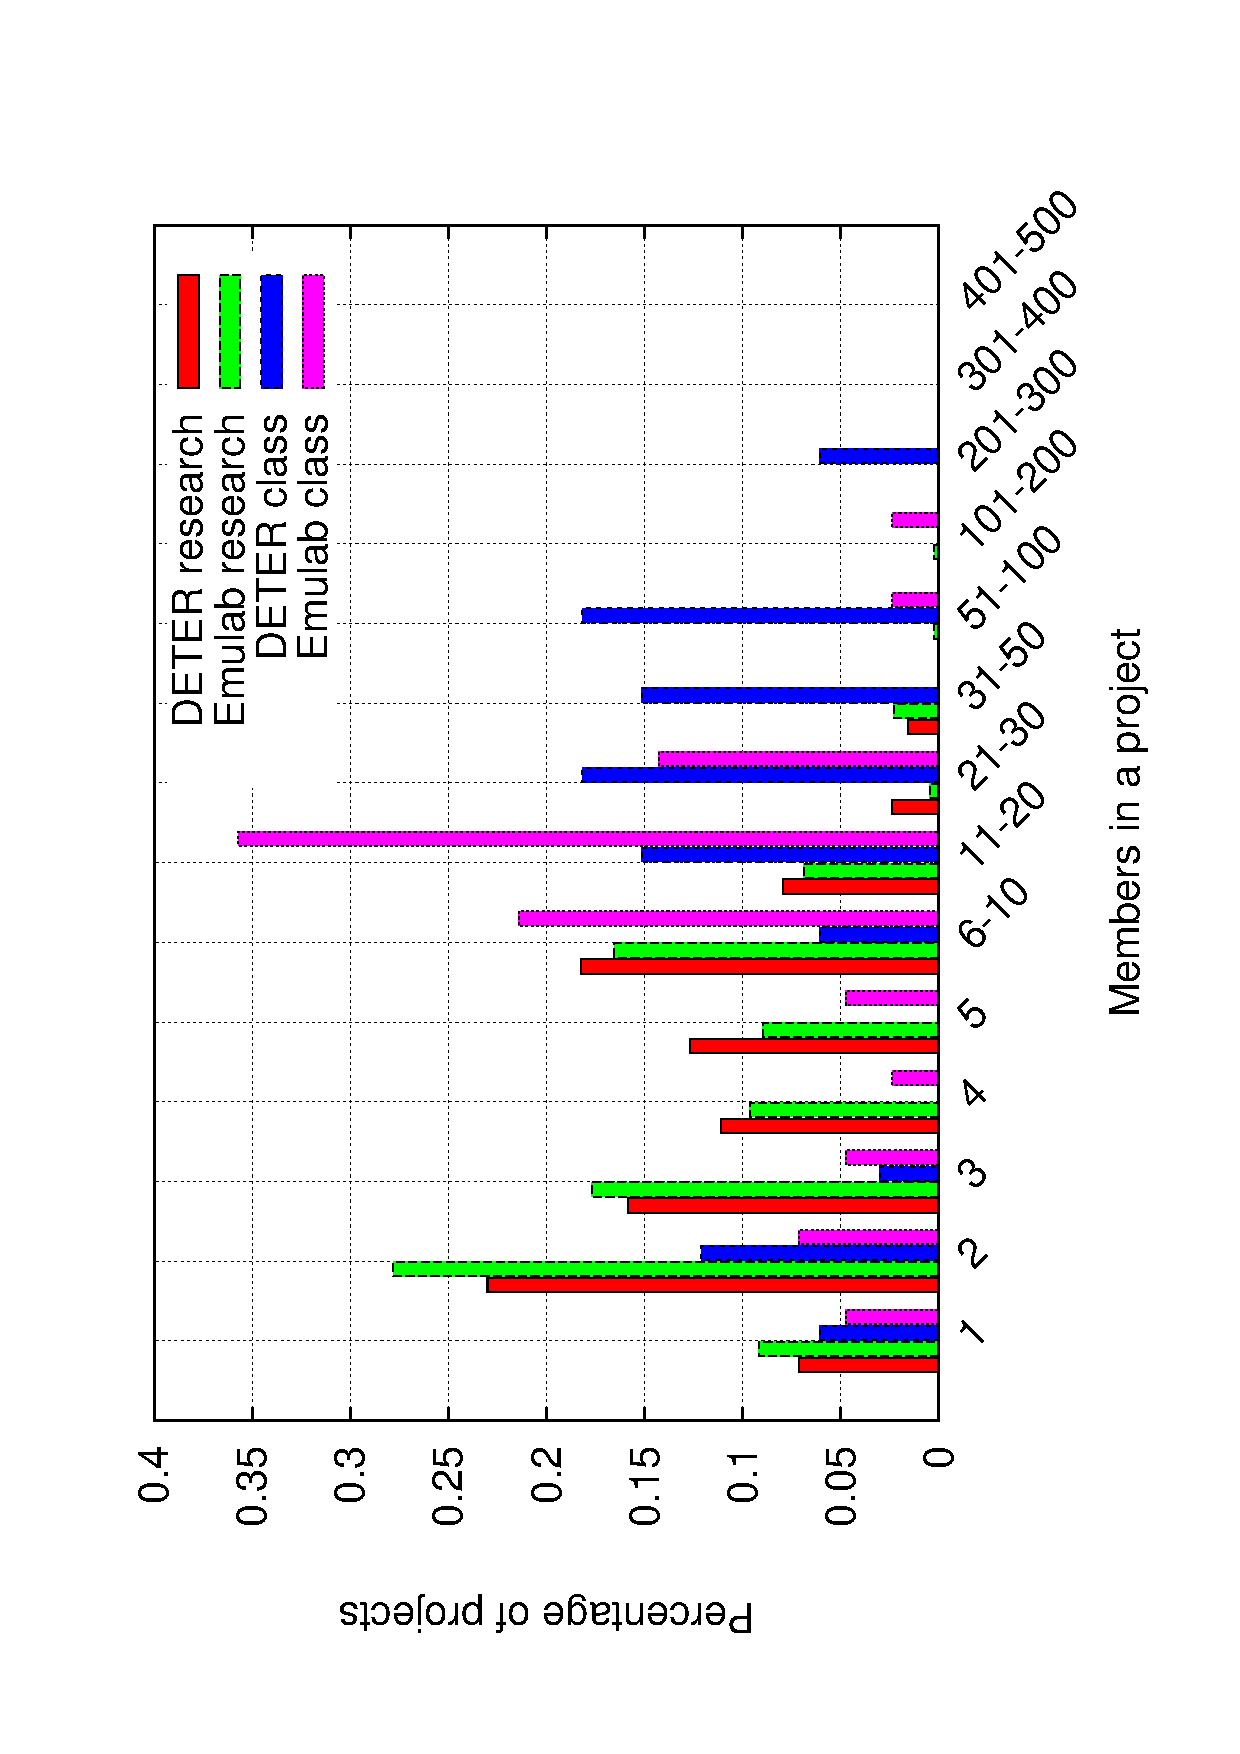
\includegraphics[width=3in,
type=pdf,ext=.pdf,read=.pdf]{figs/proj.user.gnu}
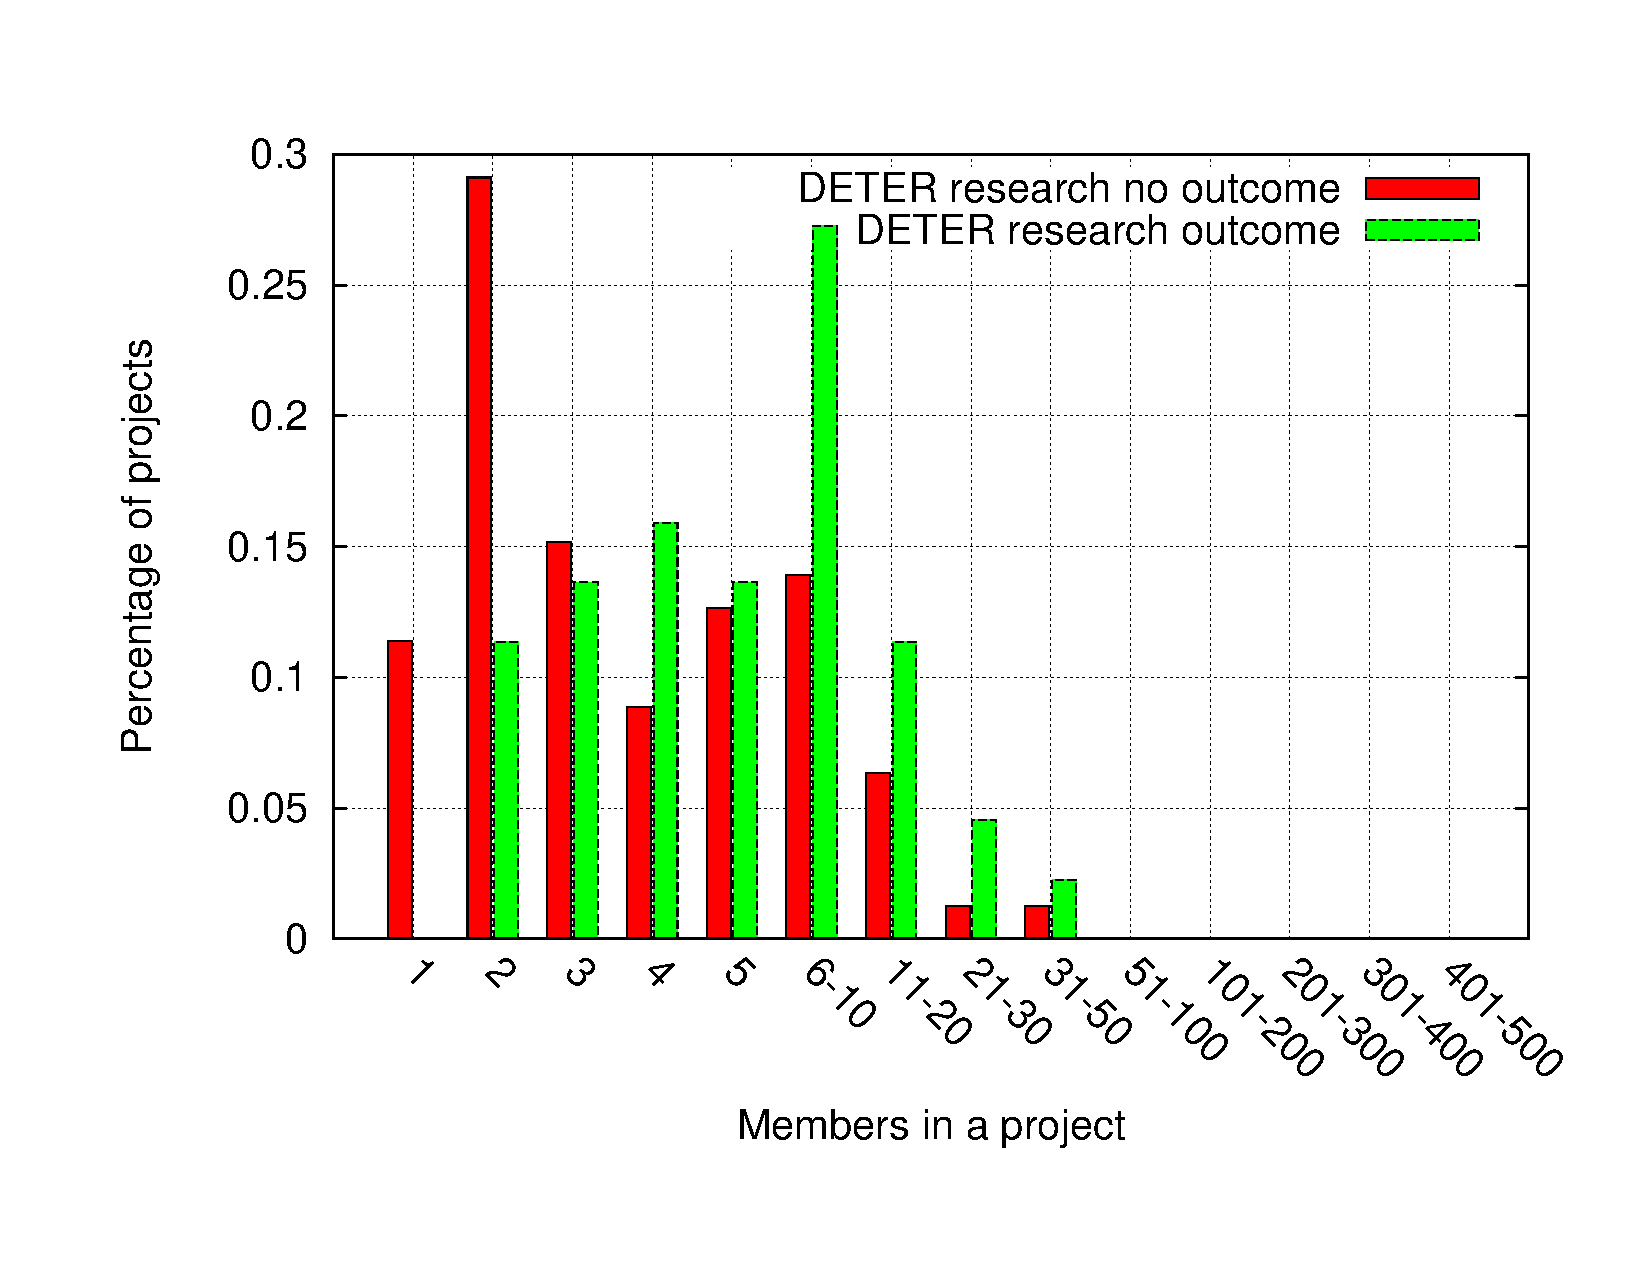
\includegraphics[width=3in,
type=pdf,ext=.pdf,read=.pdf]{figs/proj.user.cmp.gnu} \caption{Members
per project. Left: DETER vs Emulab, Right: All vs outcome}
\label{projuser} \end{center} \end{figure*}

\begin{figure*}[htbp] \begin{center} 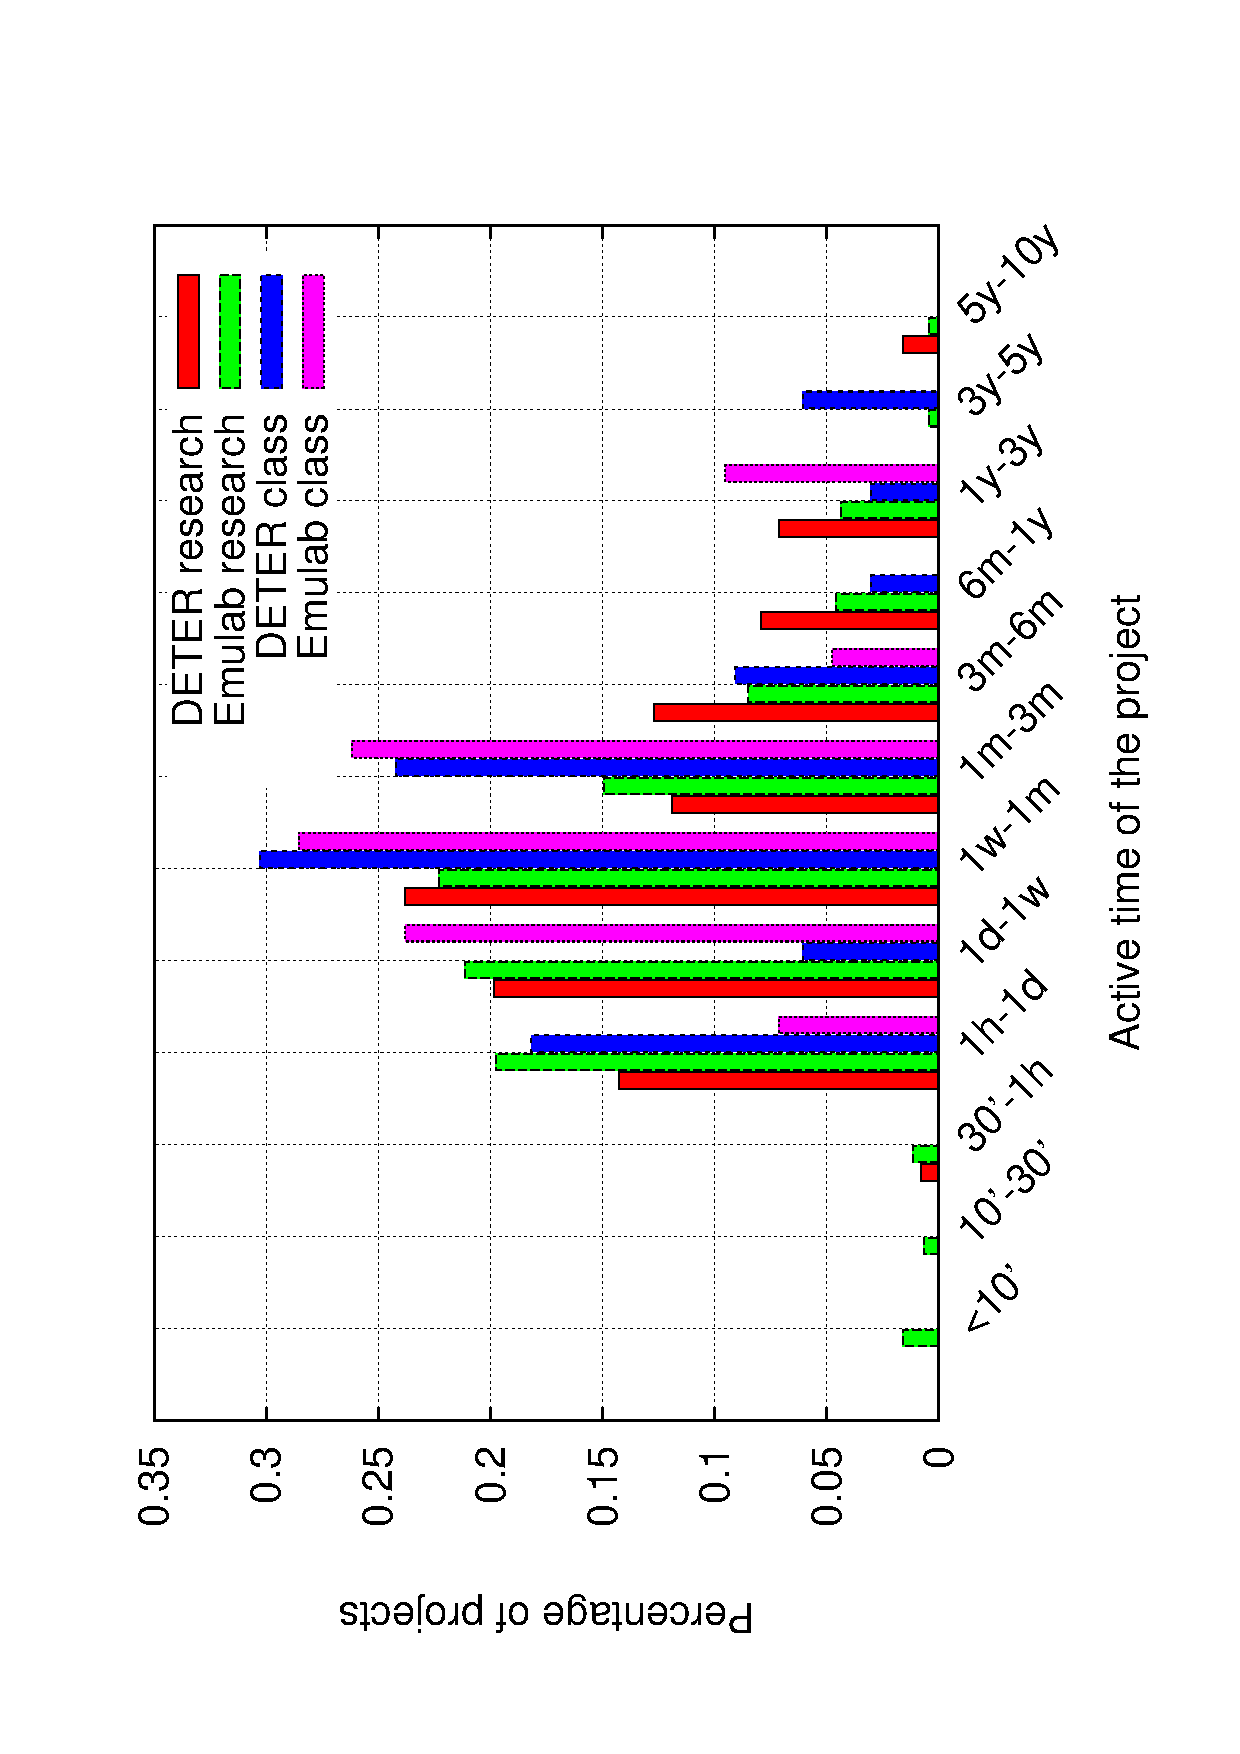
\includegraphics[width=3in,
type=pdf,ext=.pdf,read=.pdf]{figs/proj.active.gnu}
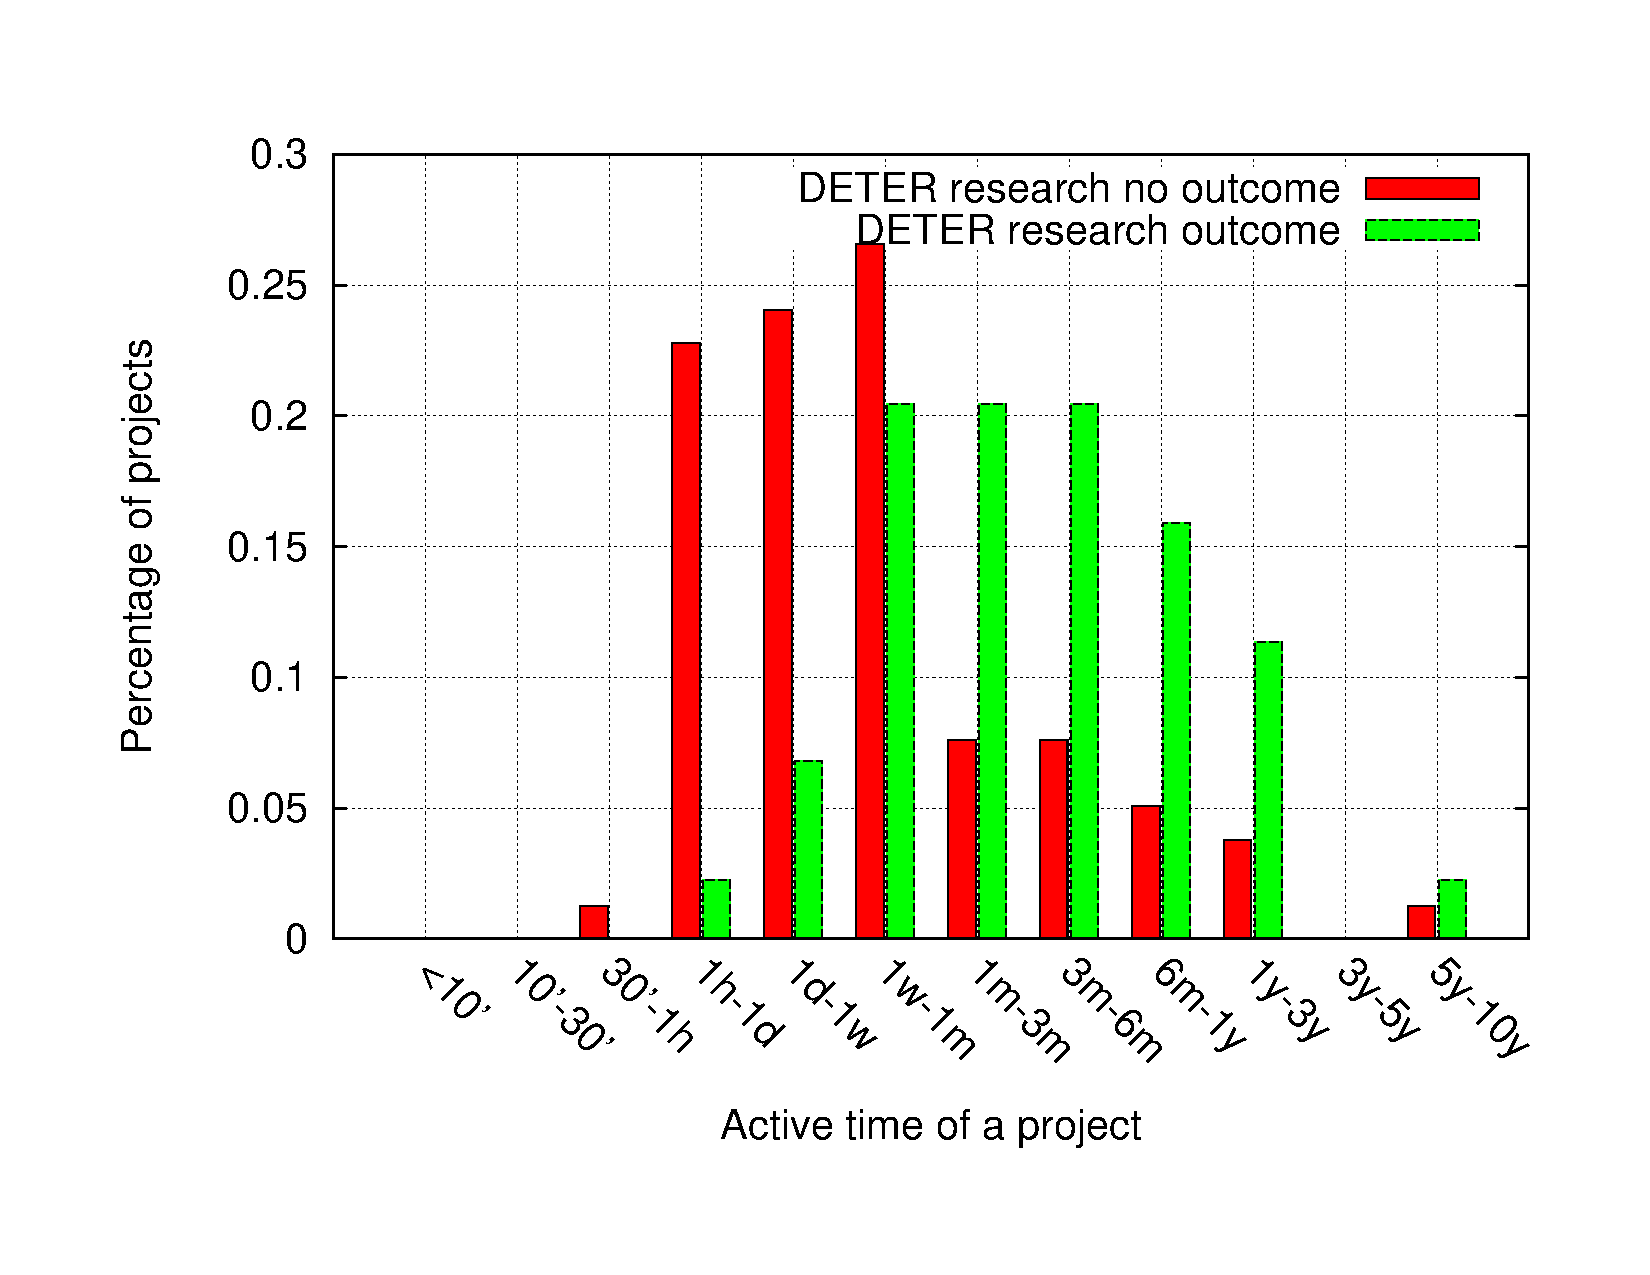
\includegraphics[width=3in,
type=pdf,ext=.pdf,read=.pdf]{figs/proj.active.cmp.gnu} \caption{Active
time of a project. Left: DETER vs Emulab, Right: All vs outcome}
\label{projactive} \end{center} \end{figure*}


\begin{figure*}[htbp] \begin{center} 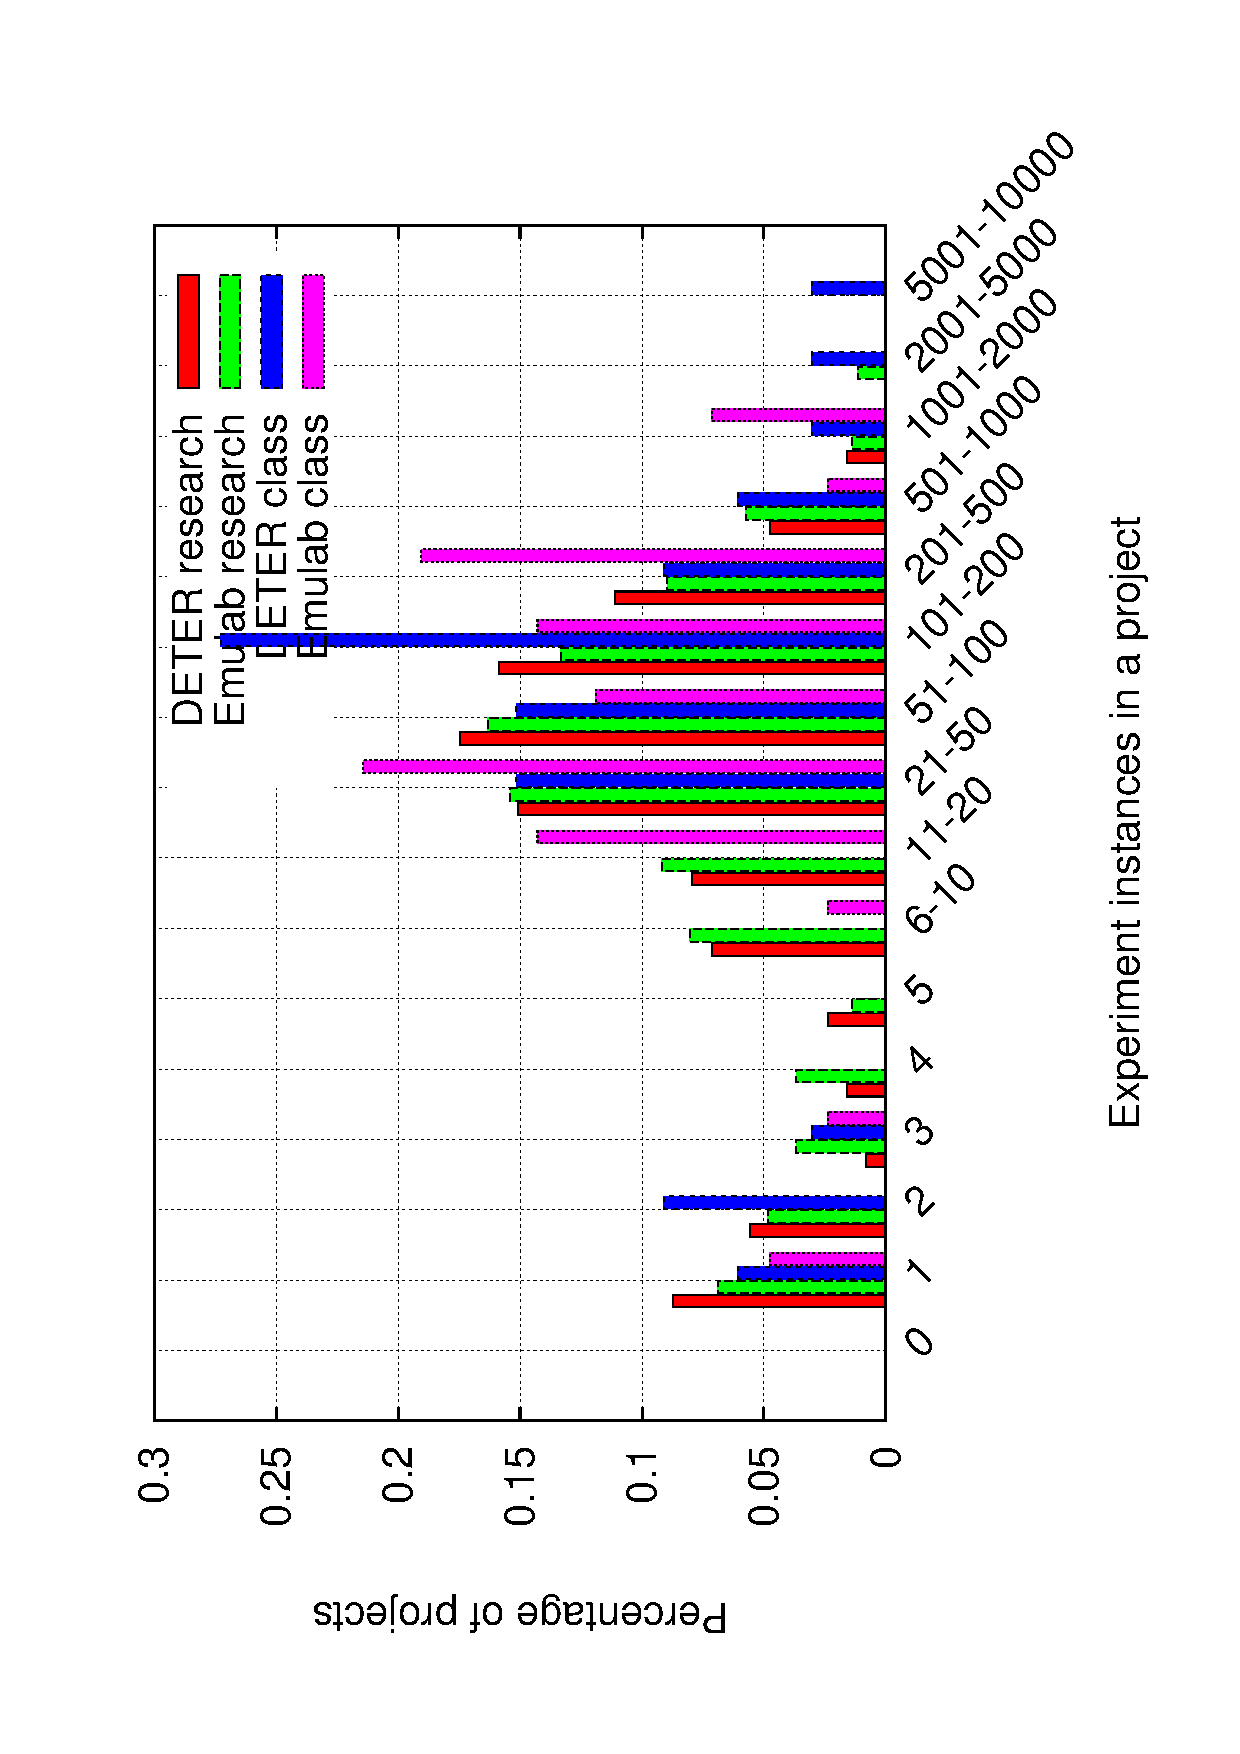
\includegraphics[width=3in,
type=pdf,ext=.pdf,read=.pdf]{figs/proj.swaps.gnu}
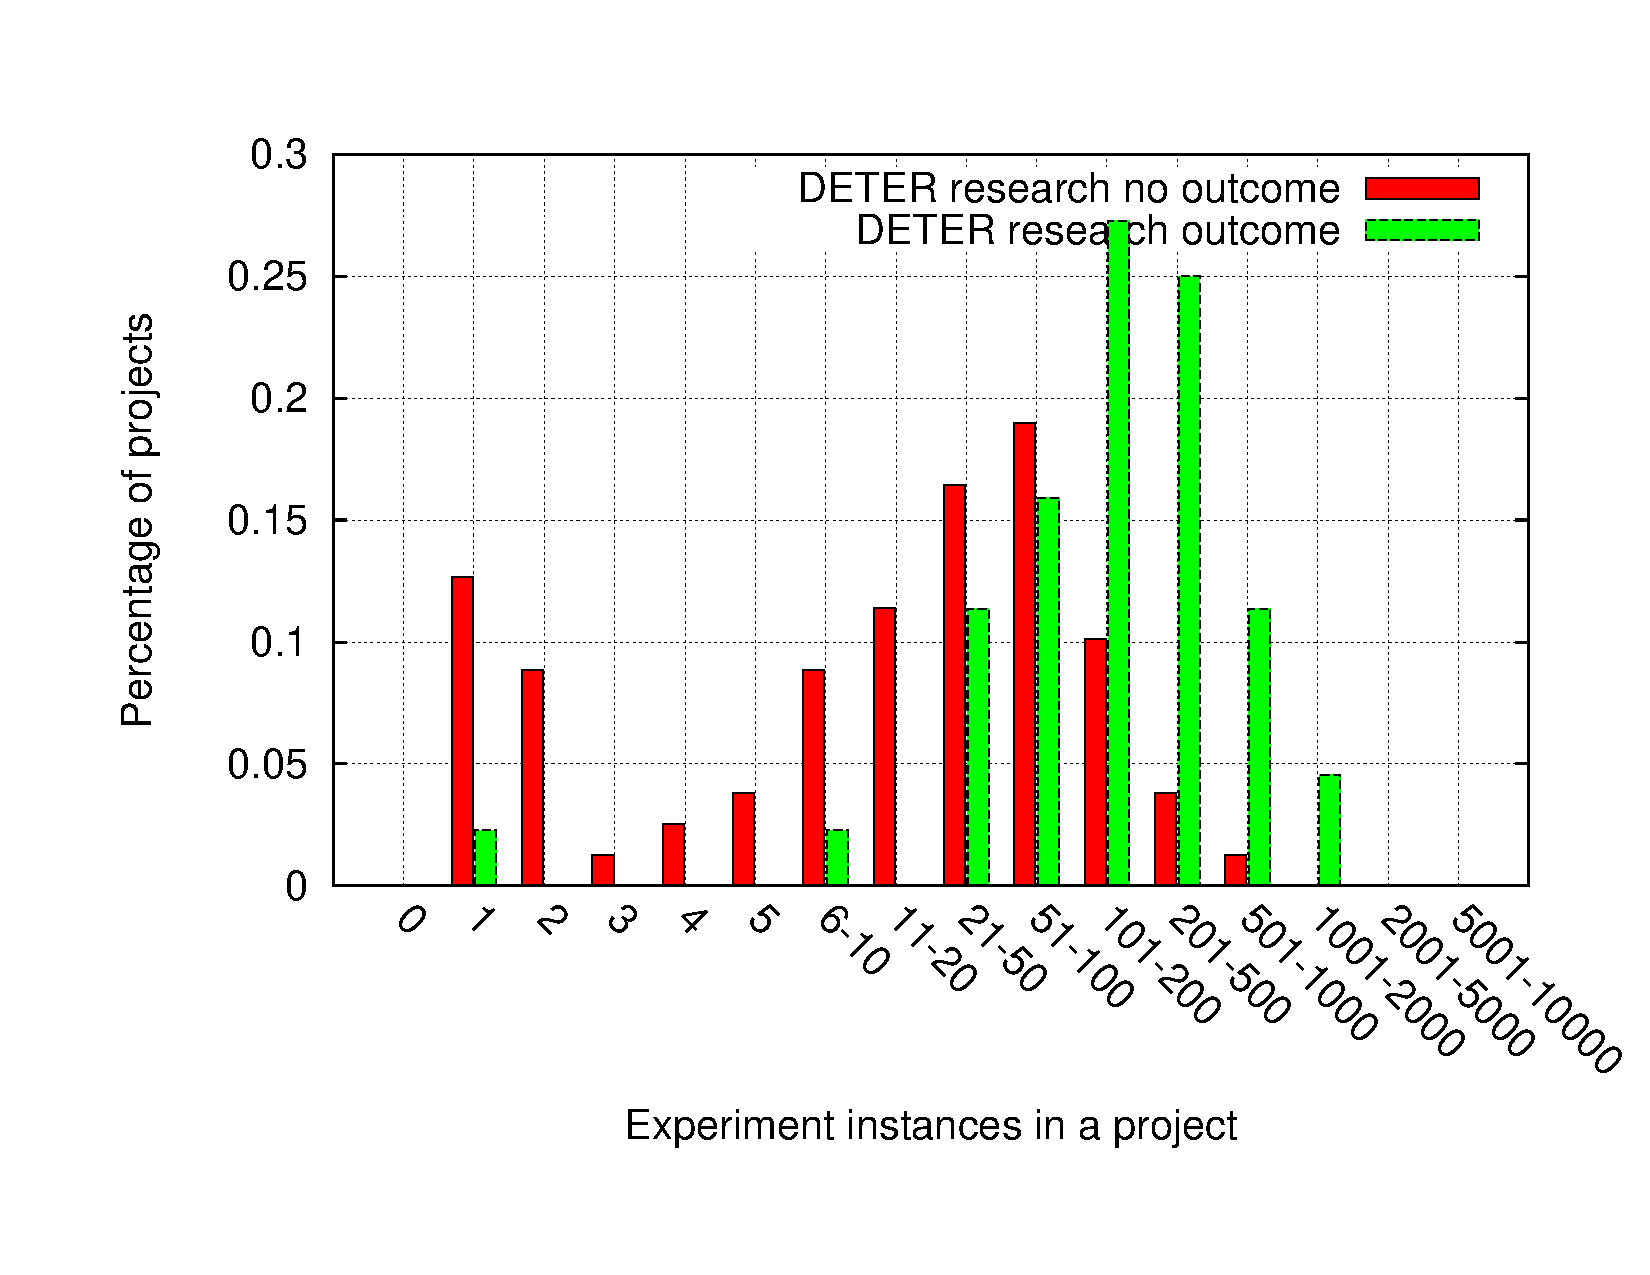
\includegraphics[width=3in,
type=pdf,ext=.pdf,read=.pdf]{figs/proj.swaps.cmp.gnu}
\caption{Experiment instances in a project. Left: DETER vs Emulab,
Right: All vs outcome} \label{projswaps} \end{center} \end{figure*}

Are outcome projects more active because they have been around longer or
because they work harder? Both. Figure \ref{projagevsactive} shows that.
Figure \ref{projuservsauser} shows that in large research projects with
outcome almost all users are active, while in smaller projects only a
few may be active. What's surprising is that for classes with outcome
sometimes only half of the users are active. This may be due to them
having a choice of using DETER vs not or maybe because we create more
accounts than needed for the class.

\begin{figure*}[htbp] \begin{center} 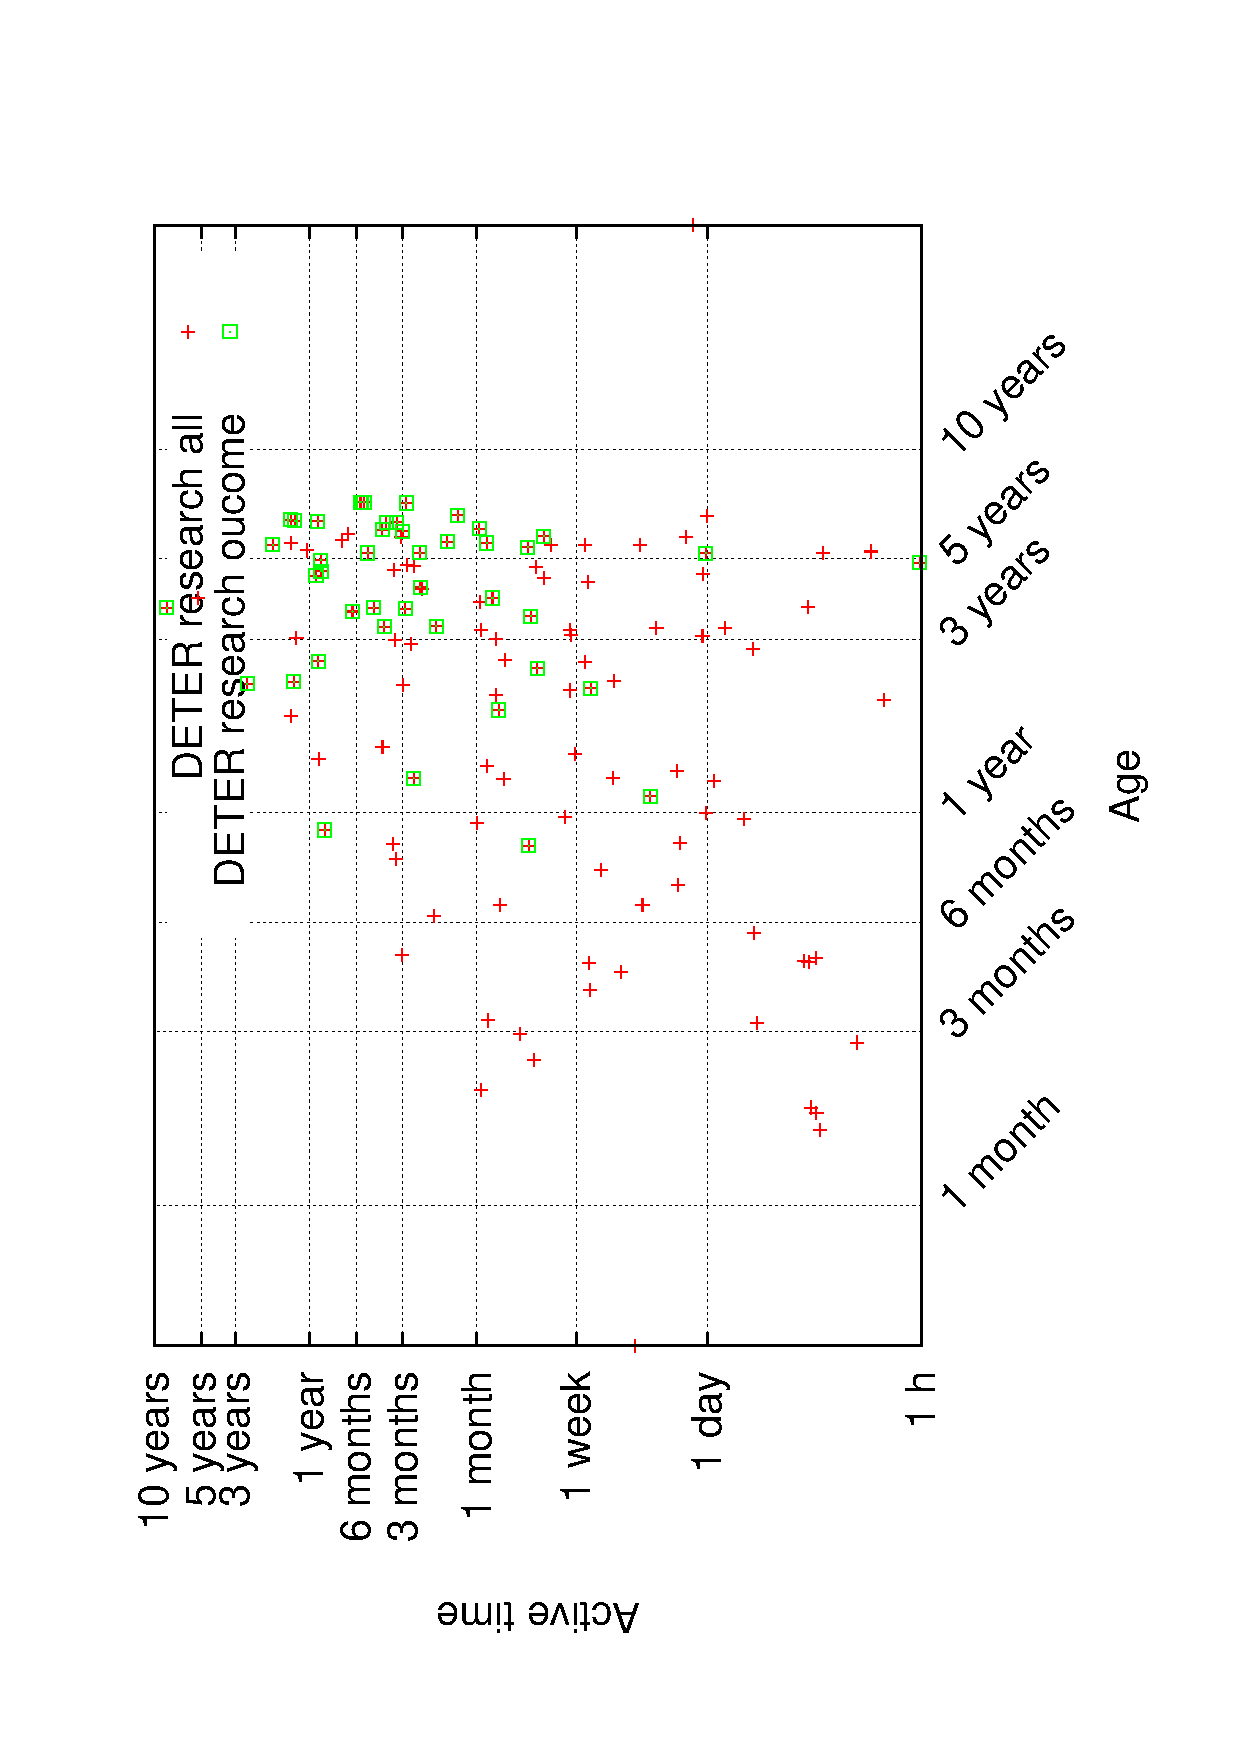
\includegraphics[width=3in,
type=pdf,ext=.pdf,read=.pdf]{figs/proj.agevsactive.res.gnu}
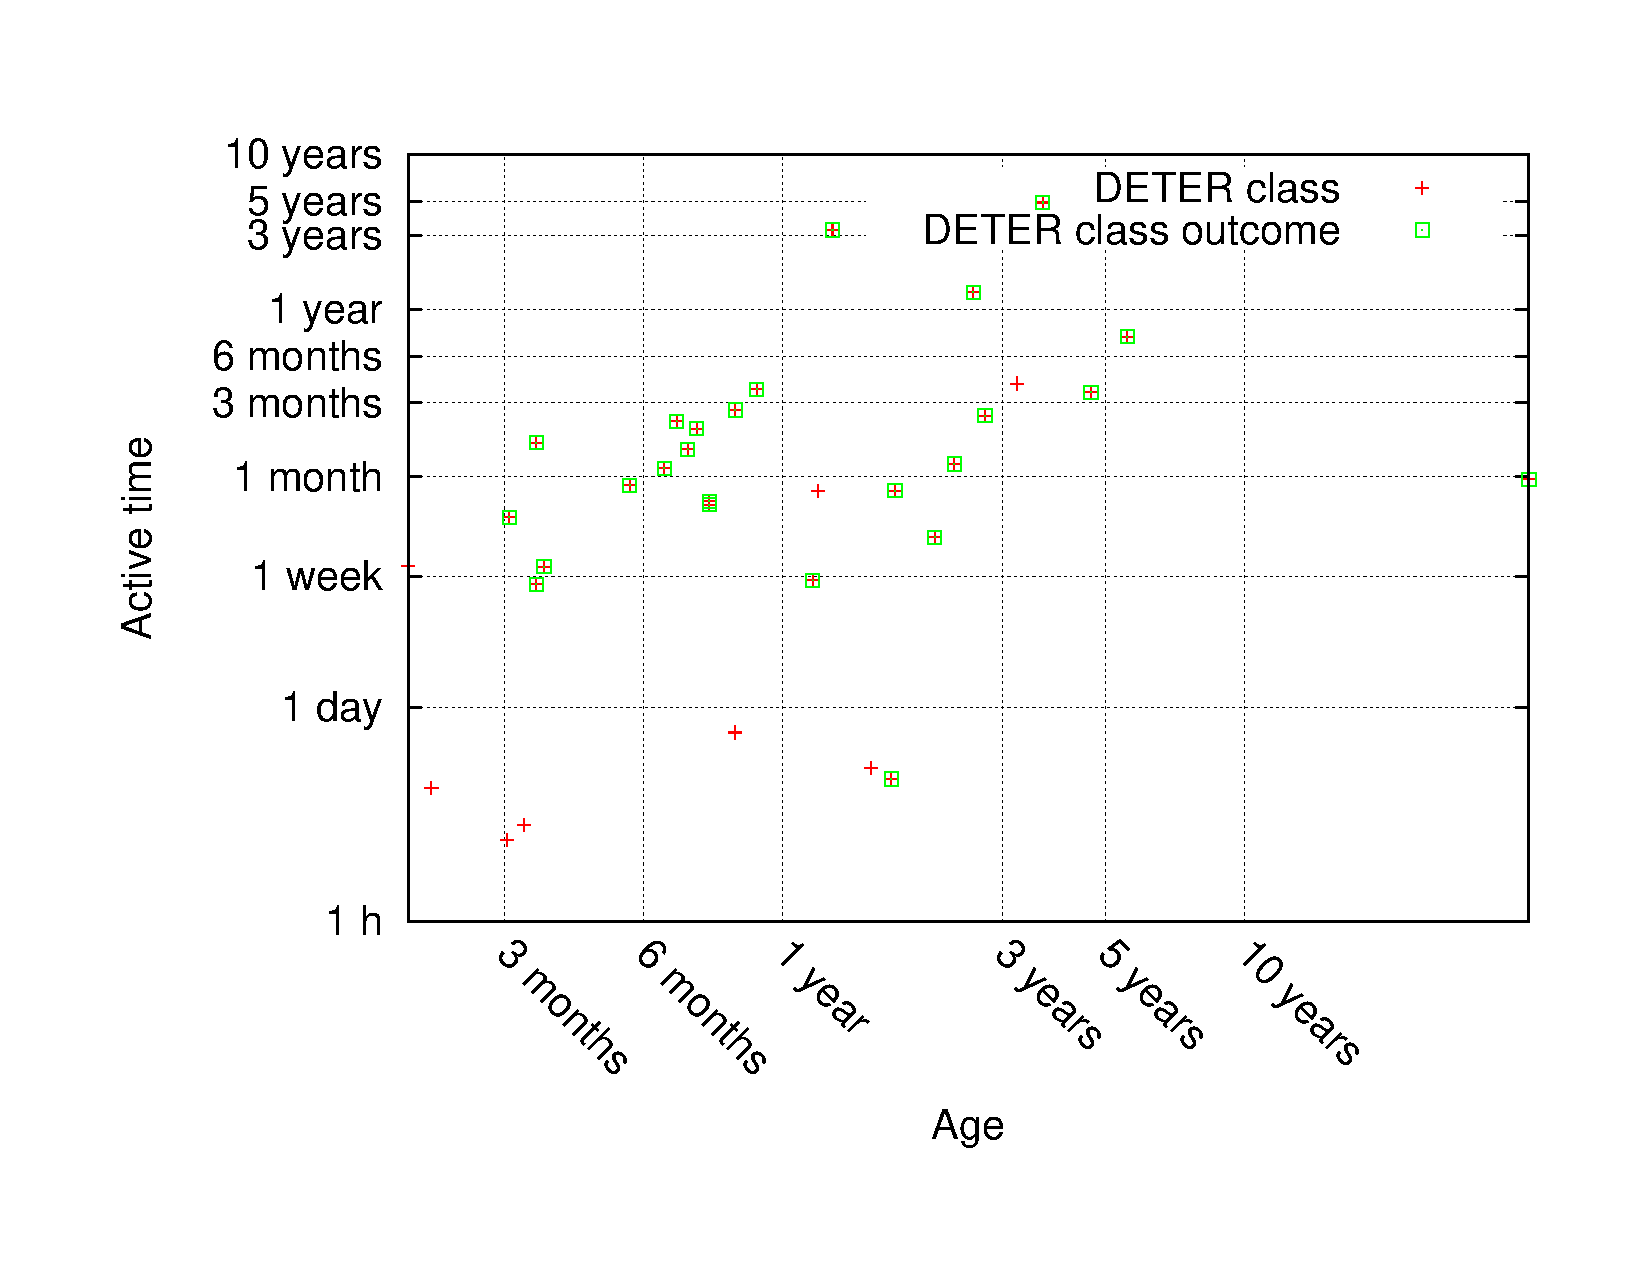
\includegraphics[width=3in,
type=pdf,ext=.pdf,read=.pdf]{figs/proj.agevsactivecl.gnu}
\caption{Active time vs age of a project. Left: DETER research, right:
DETER class} \label{projagevsactive} \end{center} \end{figure*}

\begin{figure*}[htbp] \begin{center} 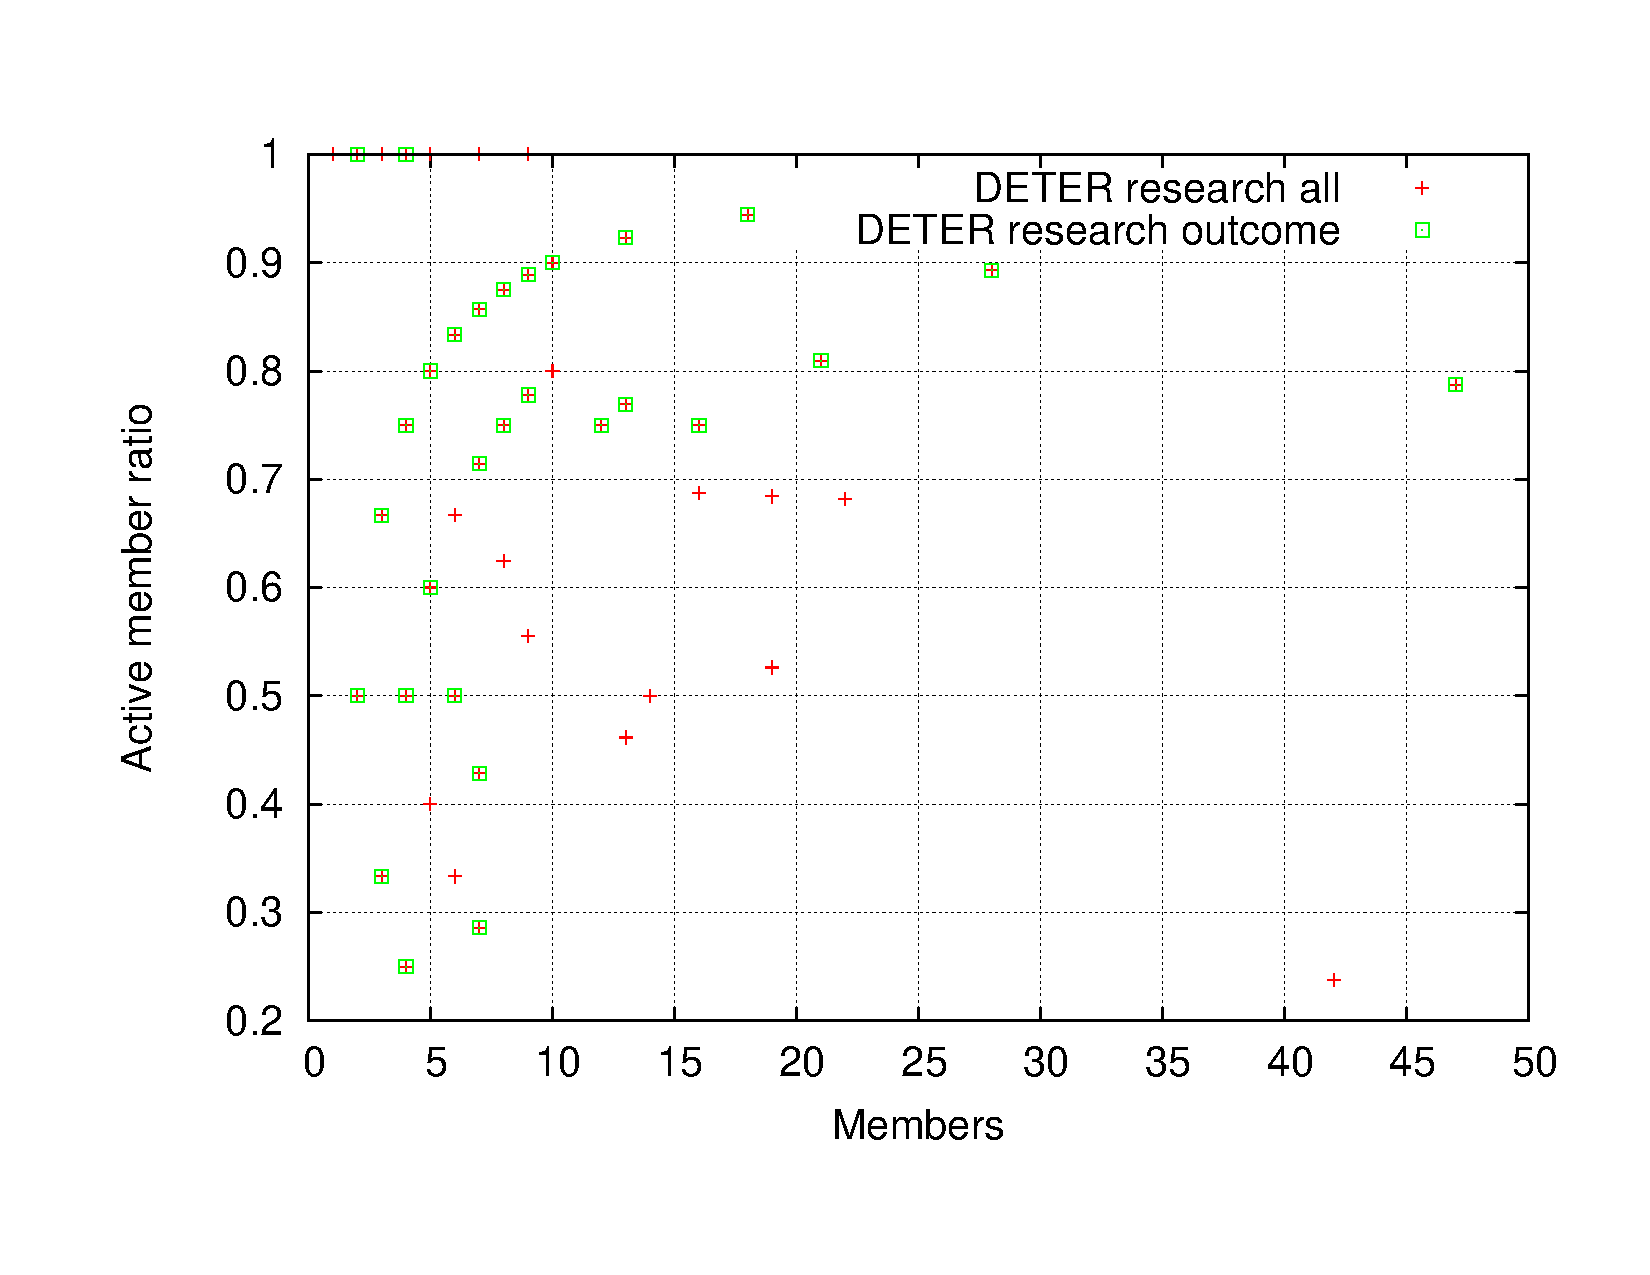
\includegraphics[width=3in,
type=pdf,ext=.pdf,read=.pdf]{figs/proj.uservsauserres.gnu}
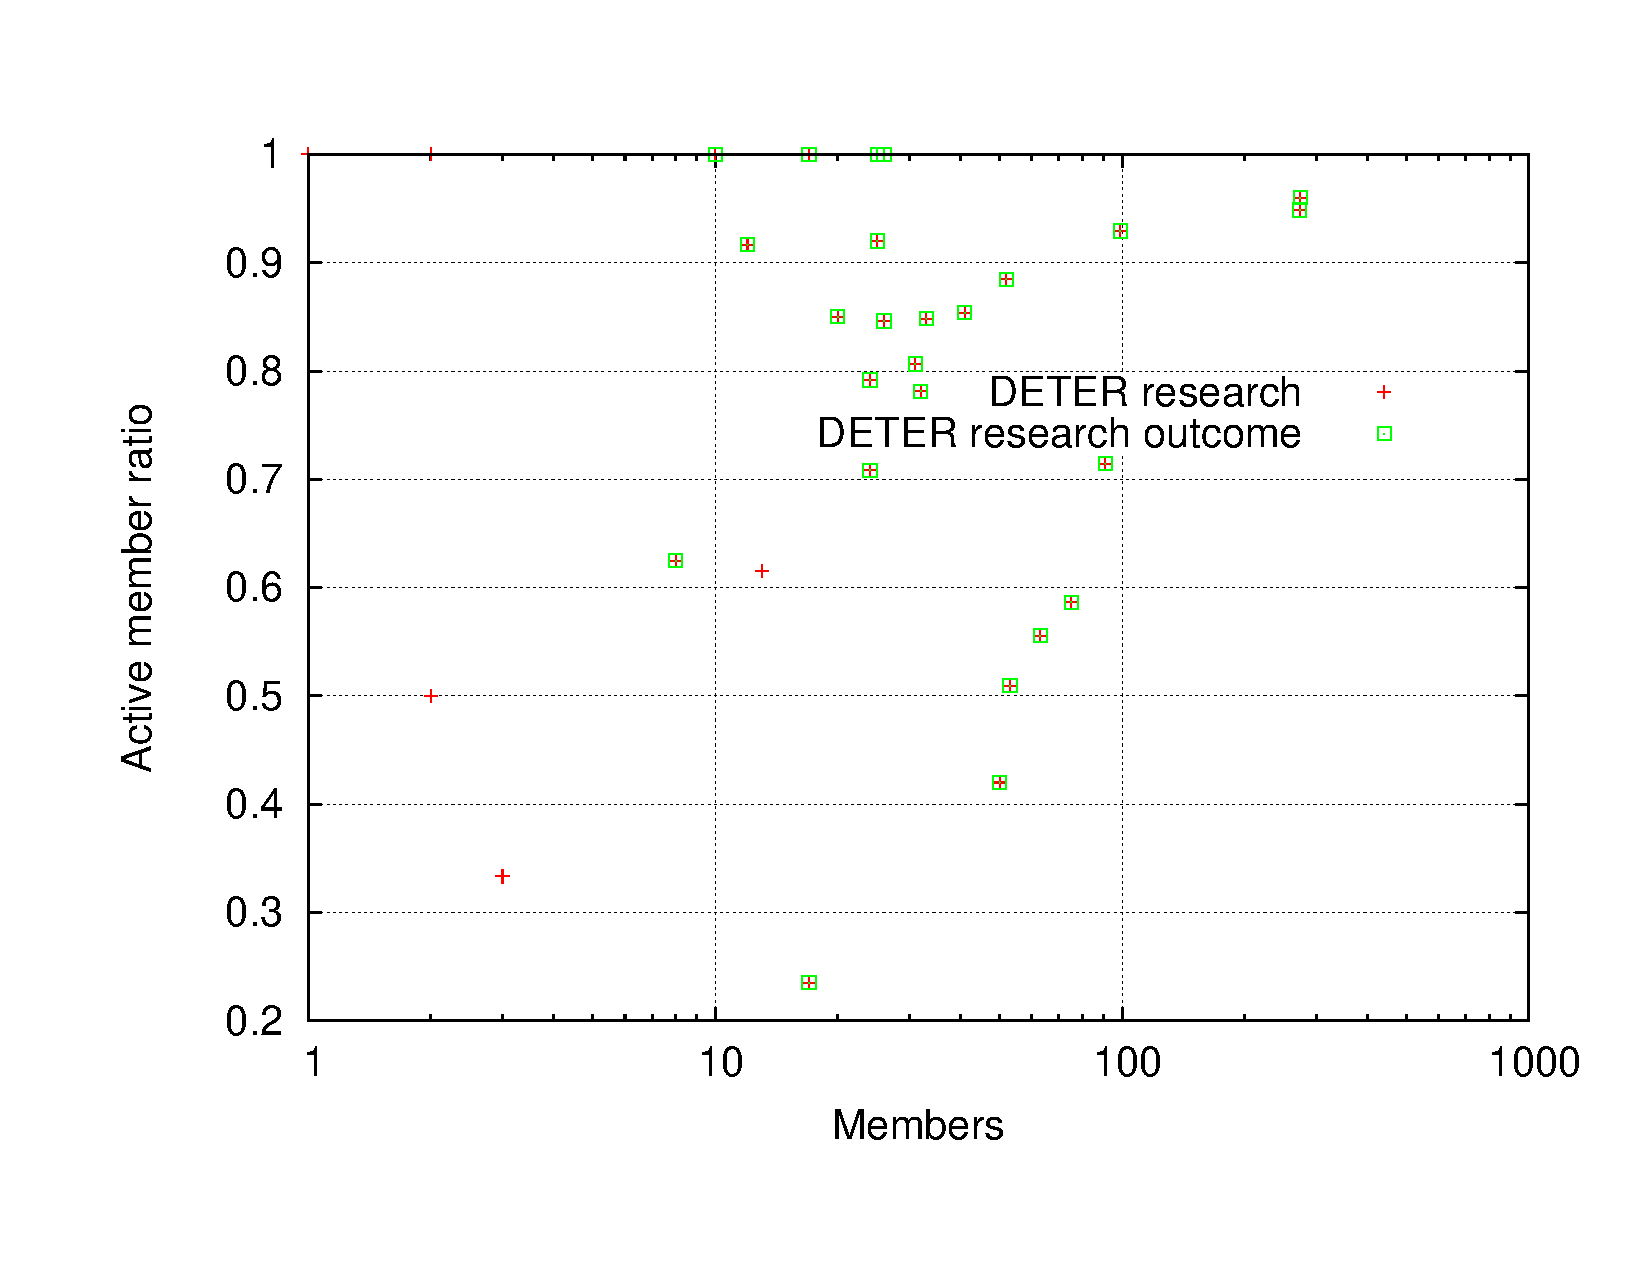
\includegraphics[width=3in,
type=pdf,ext=.pdf,read=.pdf]{figs/proj.uservsausercl.gnu}
\caption{Active member ratio vs all members of a project. Left: DETER
research, right: DETER class} \label{projuservsauser} \end{center}
\end{figure*}

Explain project evolution from inception to publication. Quantify how
many projects do not result in productive use. Some don't manipulate
experiments at all. Some are idle. Quantify this for users as well.
Quantify this for experiments and for idleness as well. Not sure if
idleness goes here.



\subsection{User Distributions} 


\begin{figure*}[htbp] \begin{center} 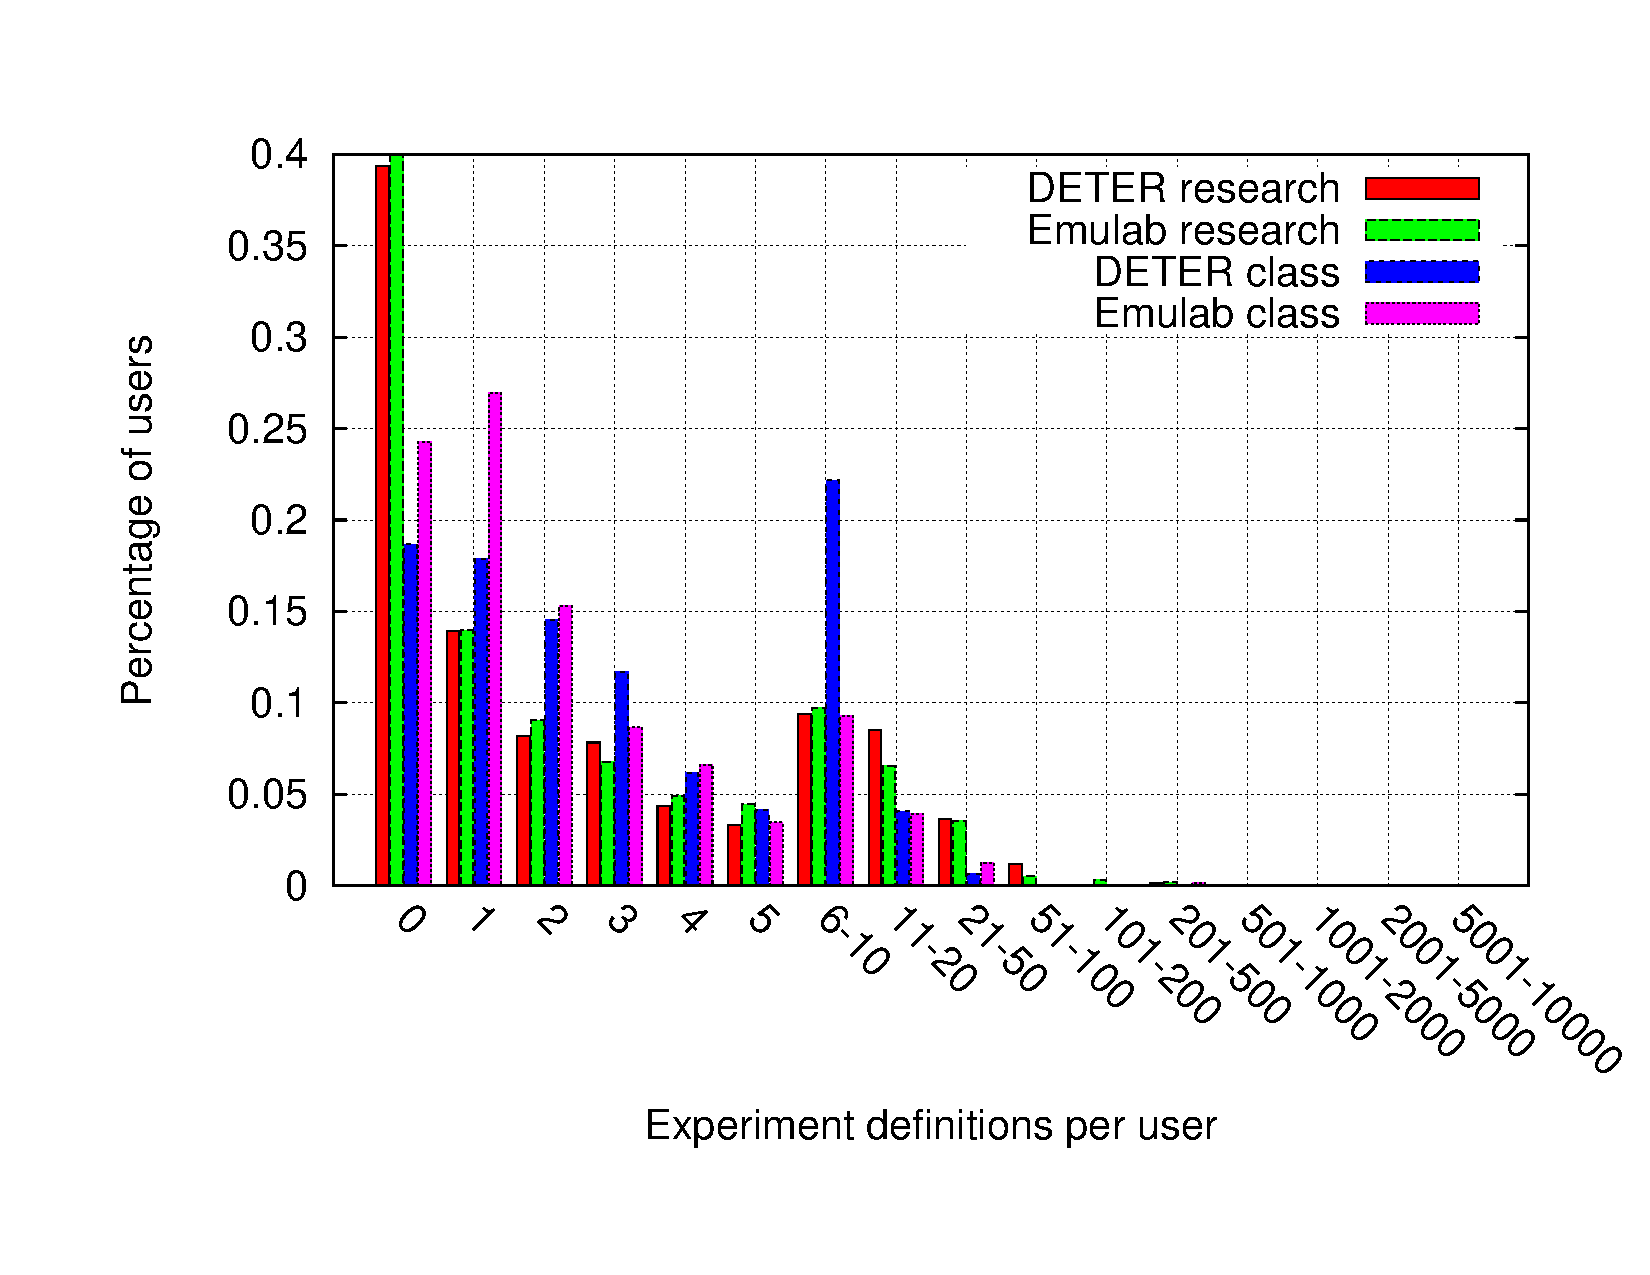
\includegraphics[width=3in,
type=pdf,ext=.pdf,read=.pdf]{figs/user.exp.gnu}
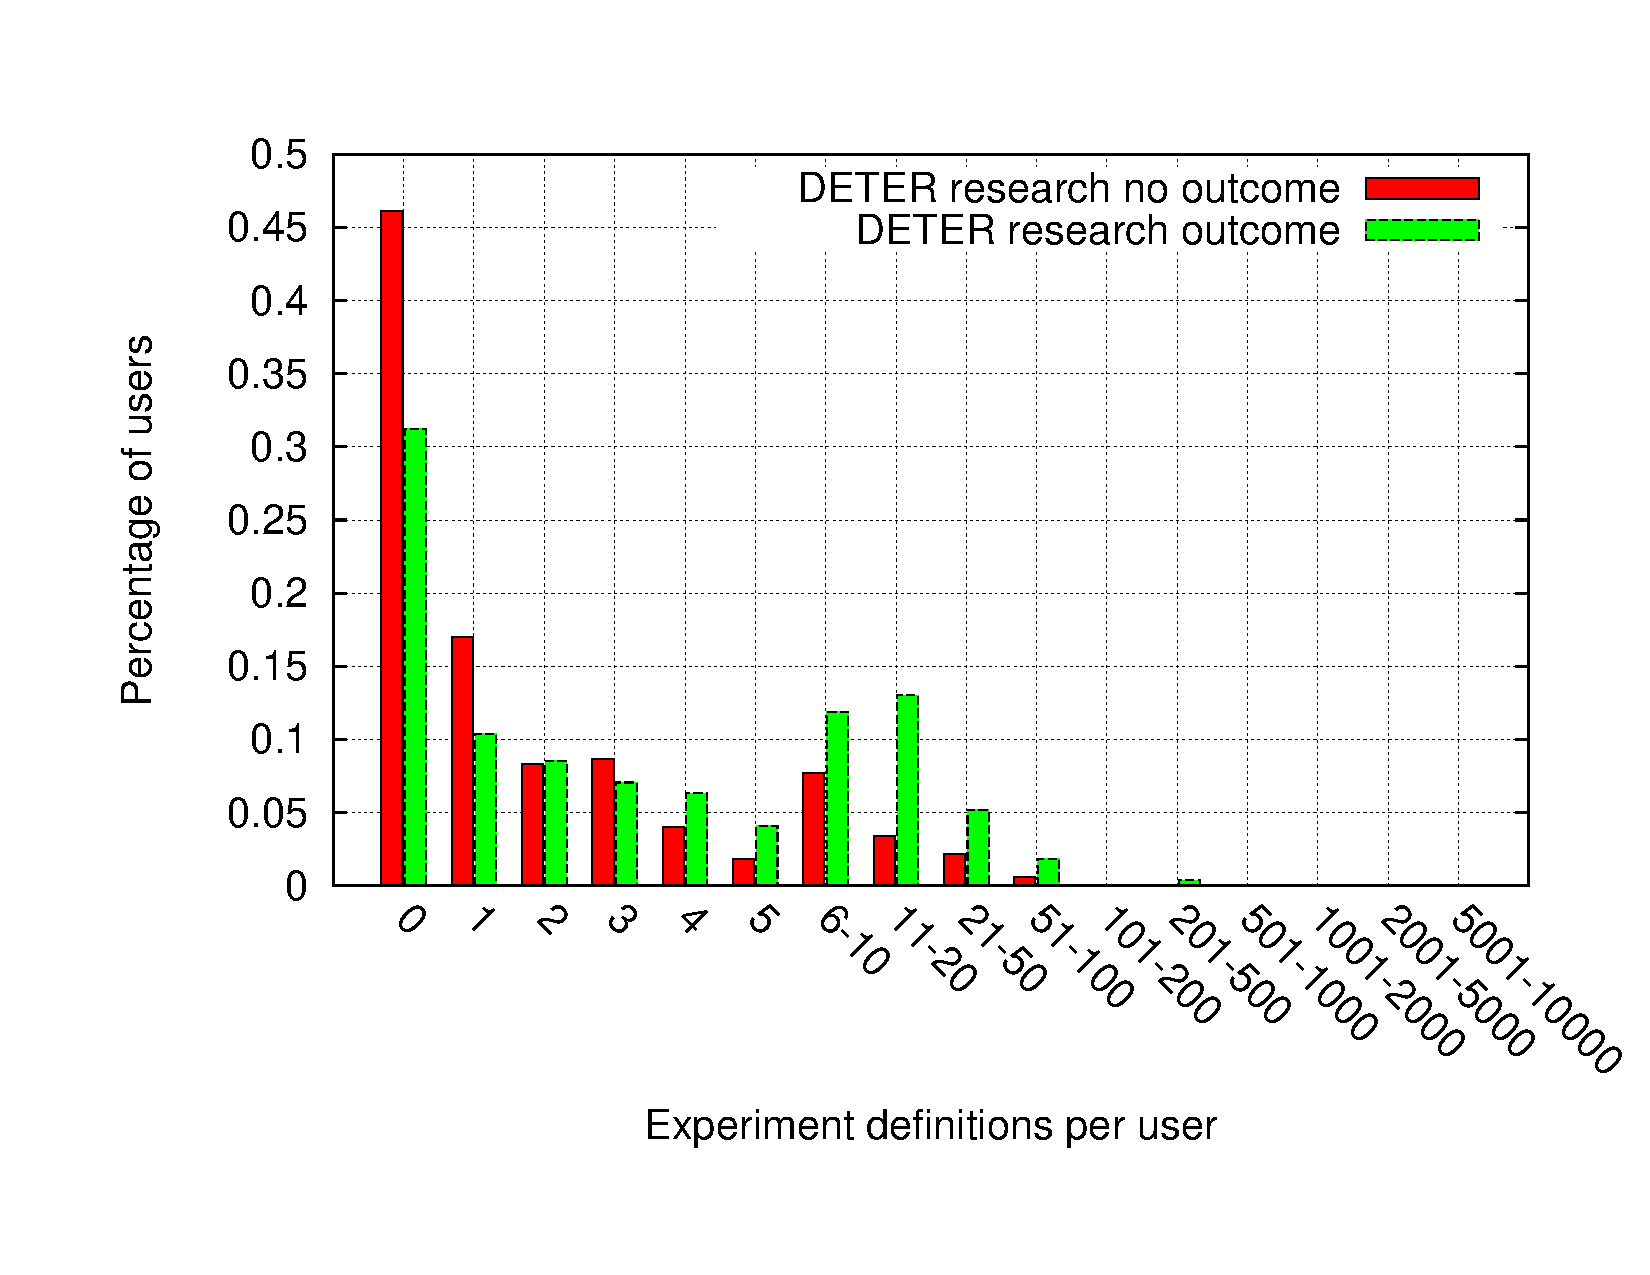
\includegraphics[width=3in,
type=pdf,ext=.pdf,read=.pdf]{figs/user.exp.cmp.gnu} 
\caption{Experiment
definitions per user. Left: DETER vs Emulab, Right: All vs outcome}
\label{userexp} \end{center} \end{figure*}

\begin{figure*}[htbp] \begin{center} 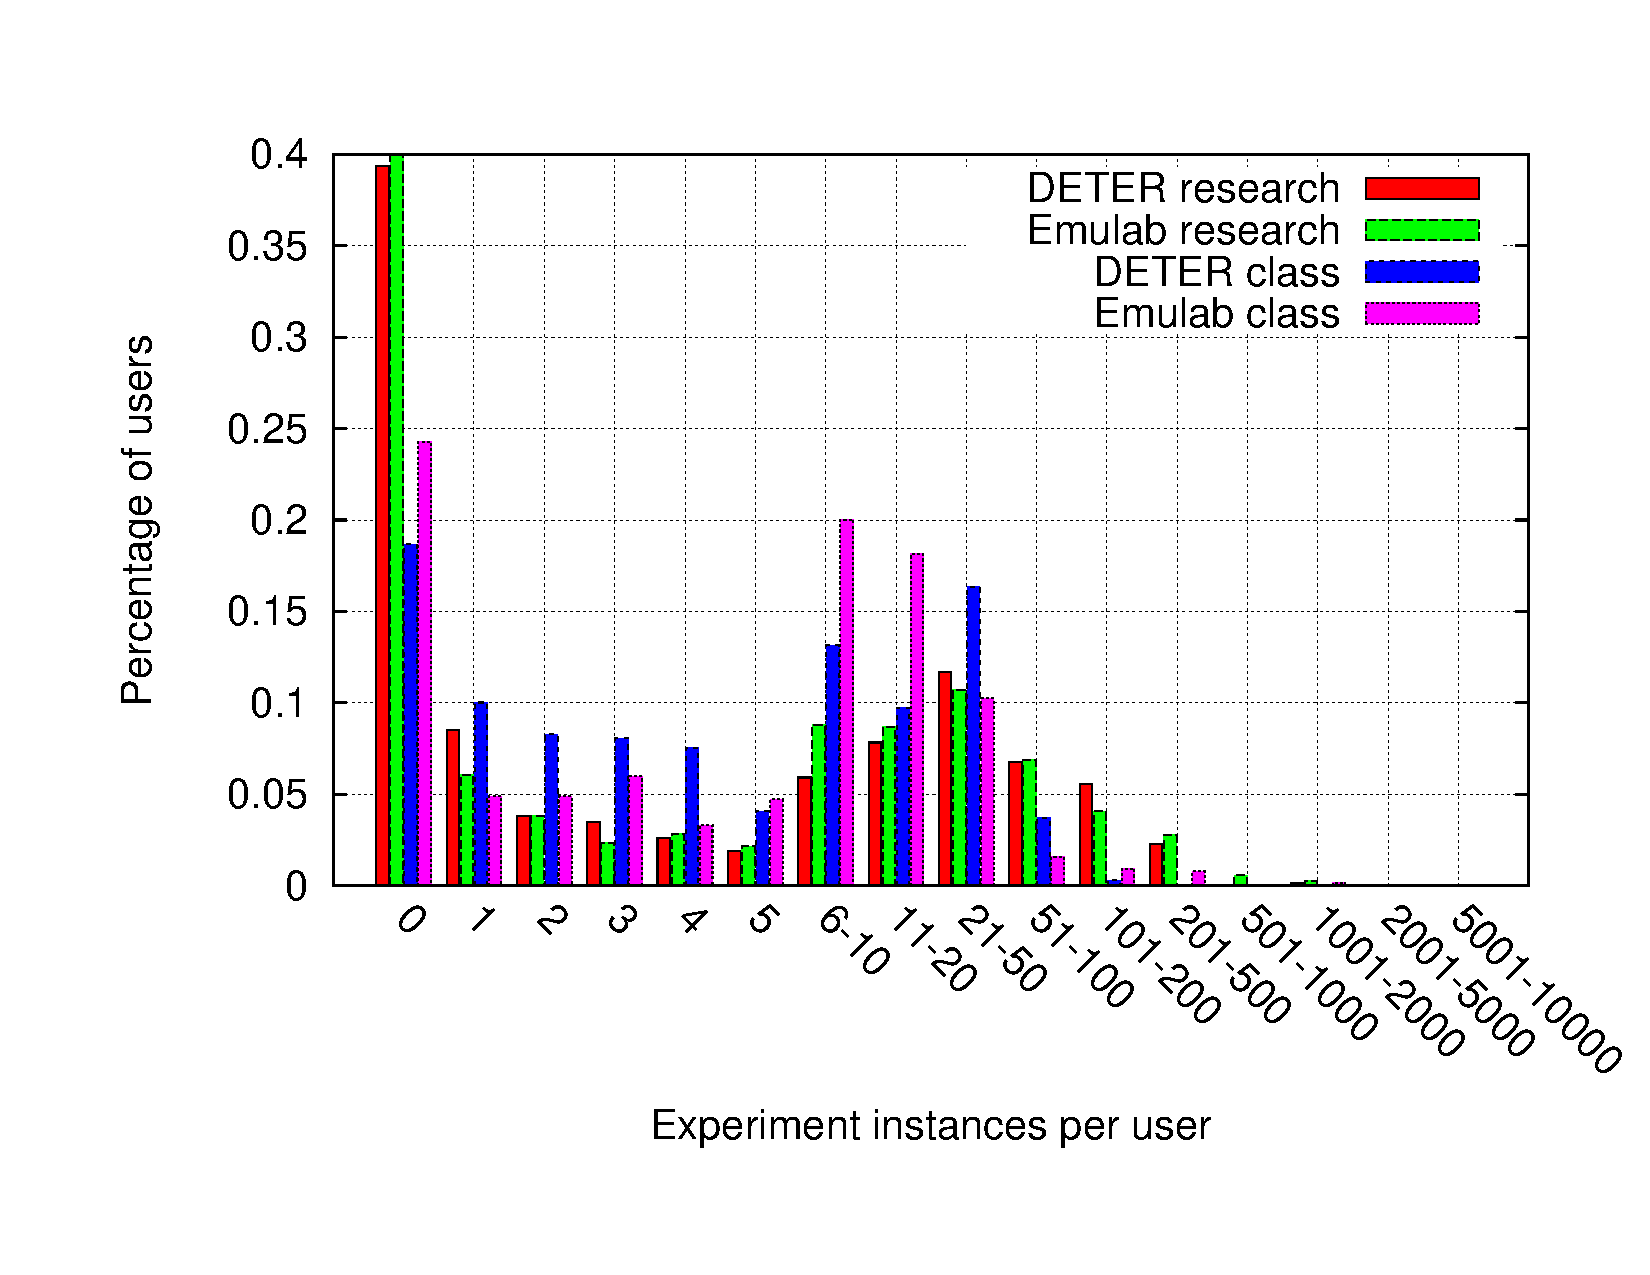
\includegraphics[width=3in,
type=pdf,ext=.pdf,read=.pdf]{figs/user.swaps.gnu}
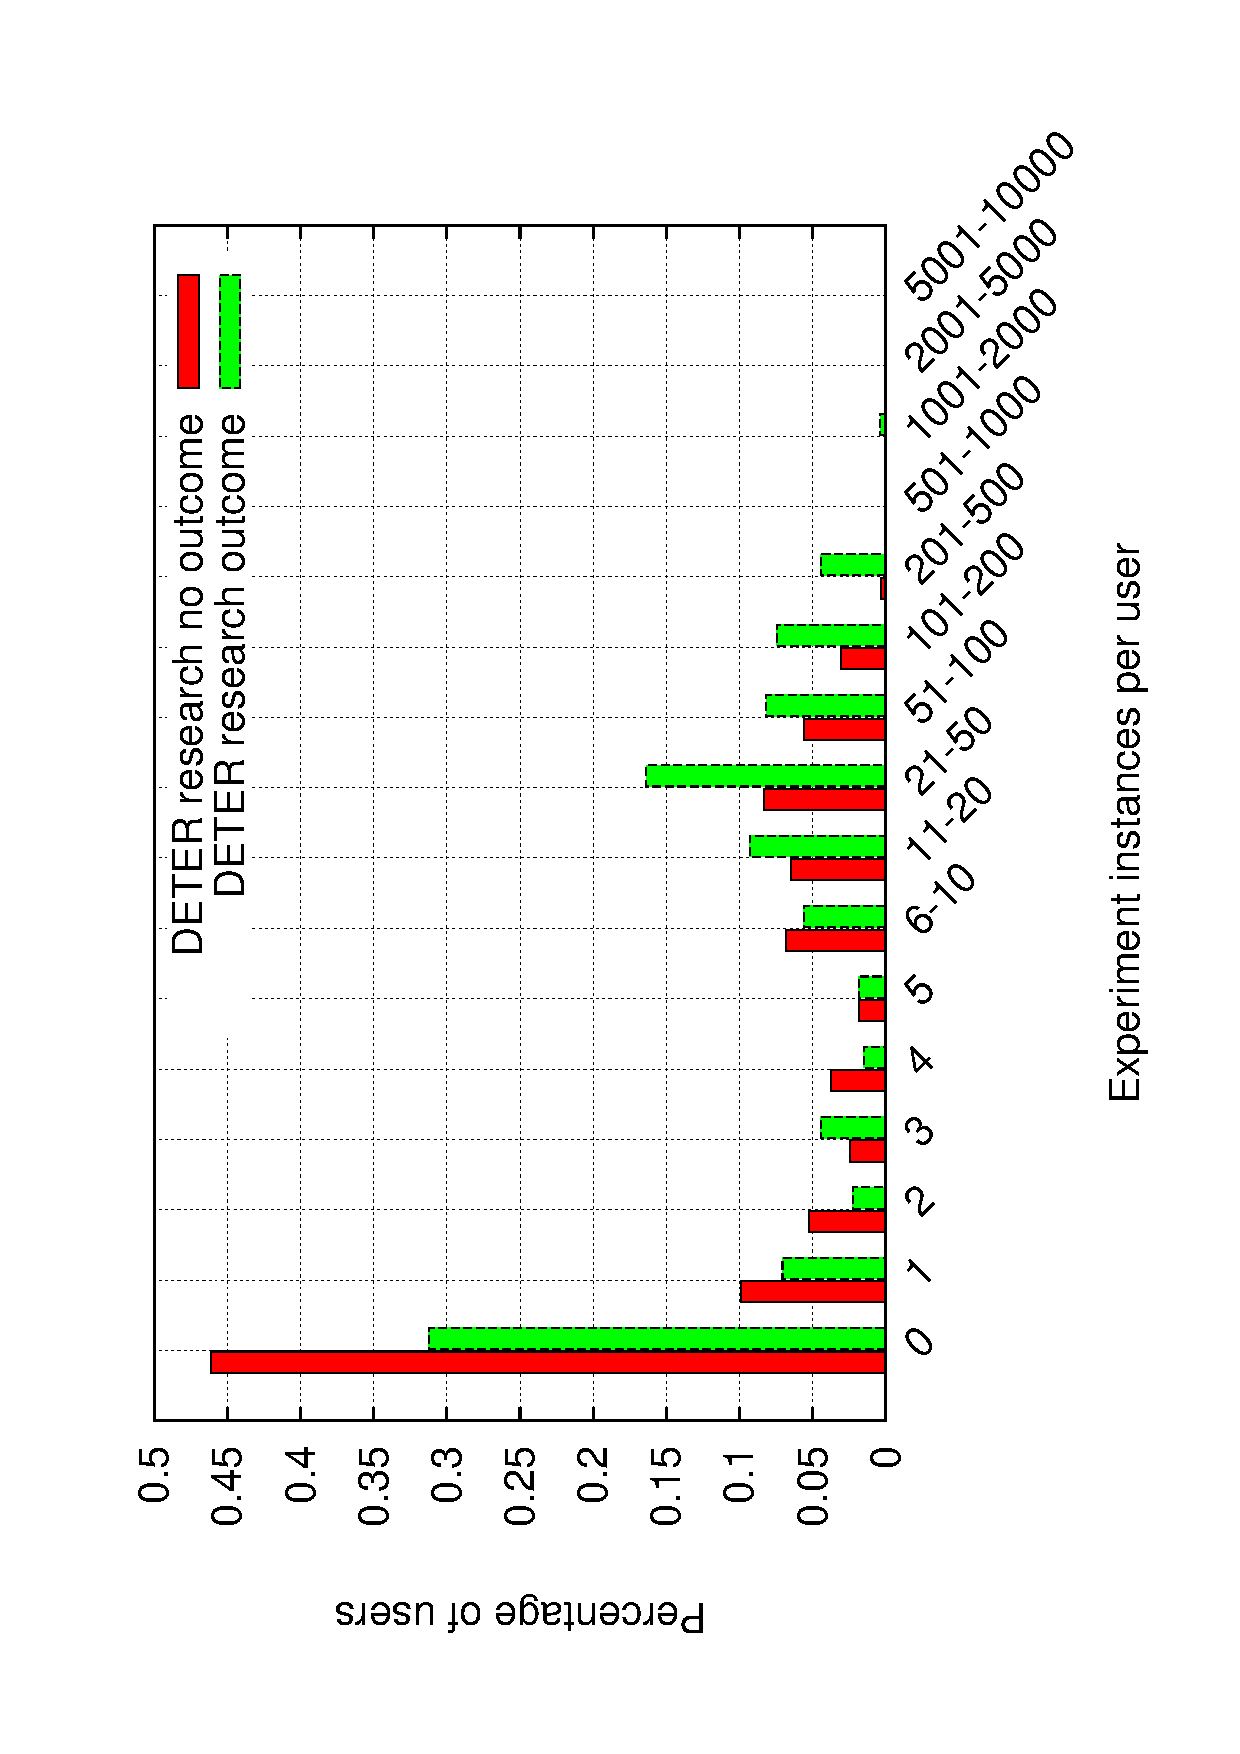
\includegraphics[width=3in,
type=pdf,ext=.pdf,read=.pdf]{figs/user.swaps.cmp.gnu}
\caption{Experiment instances per user. Left: DETER vs Emulab, Right:
All vs outcome} \label{userswaps} \end{center} \end{figure*}

\begin{figure*}[htbp] \begin{center} 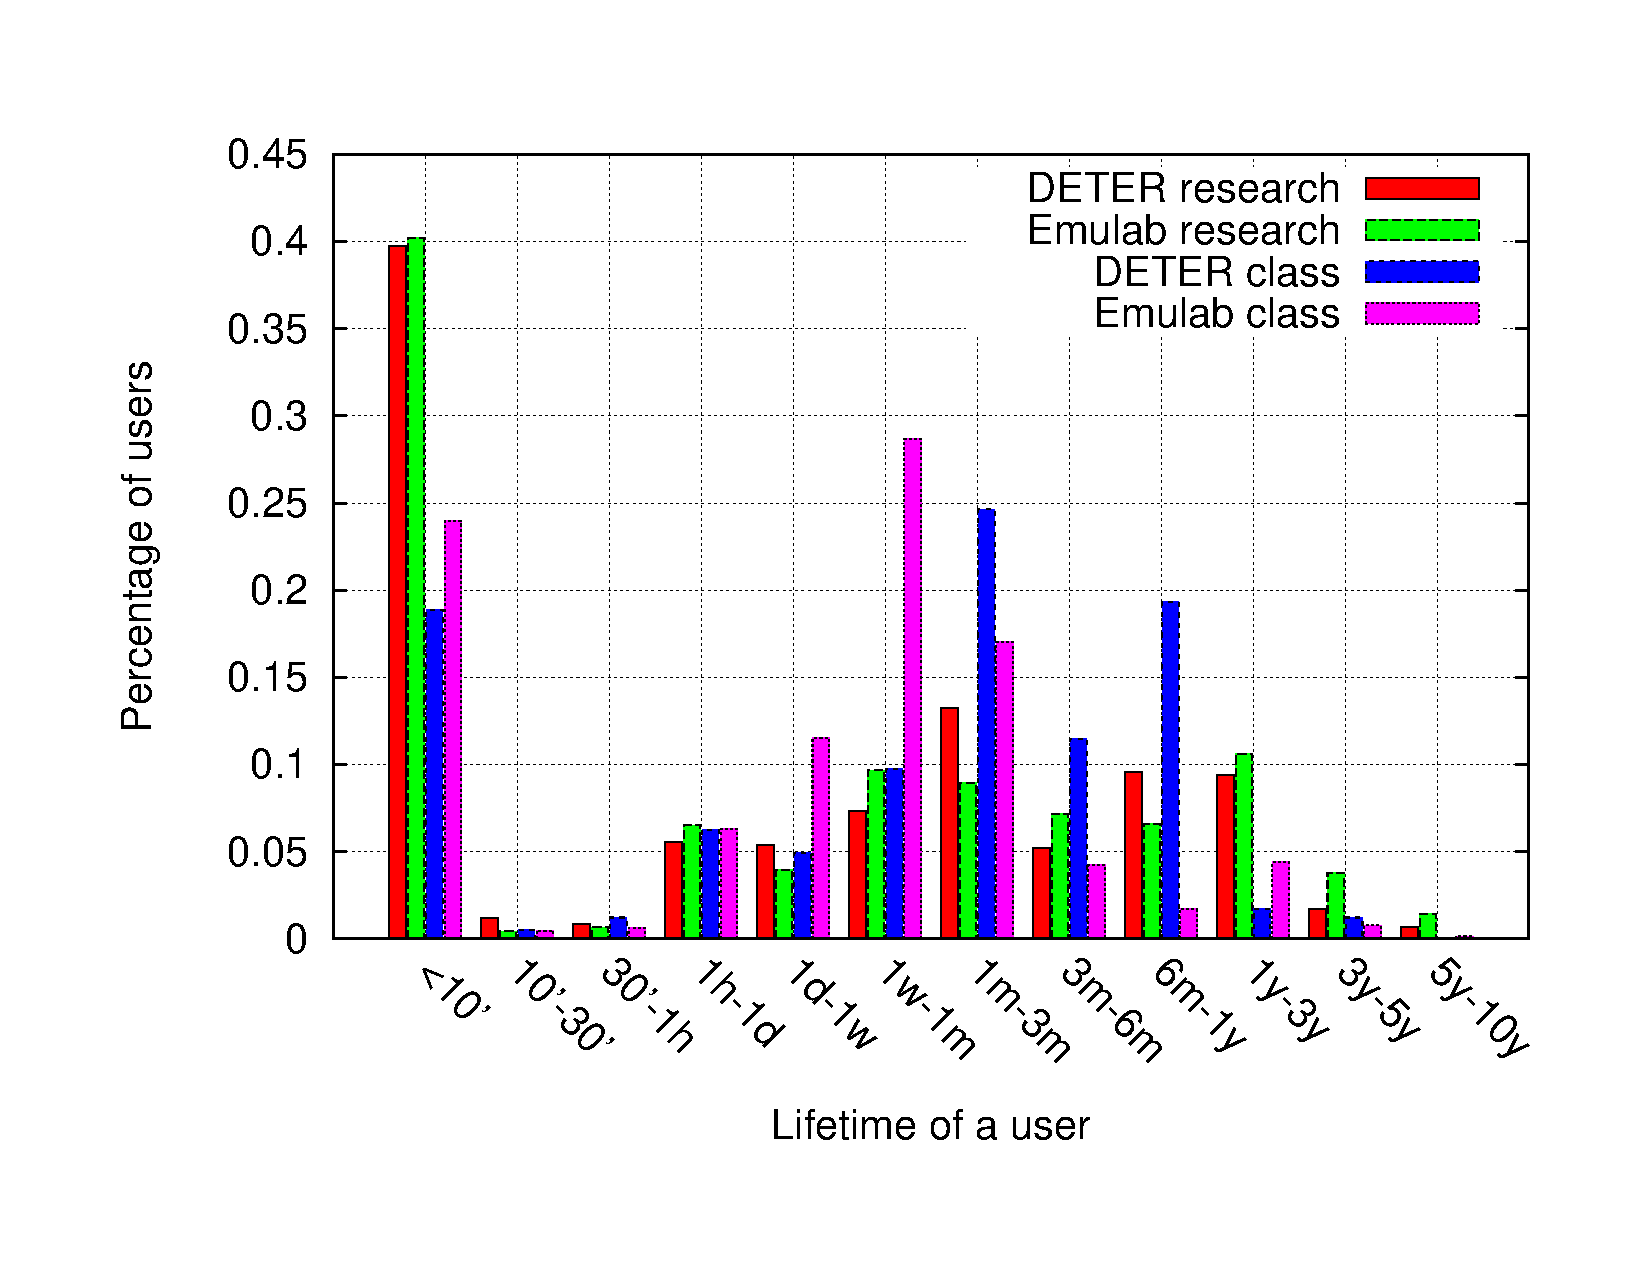
\includegraphics[width=3in,
type=pdf,ext=.pdf,read=.pdf]{figs/user.life.gnu}
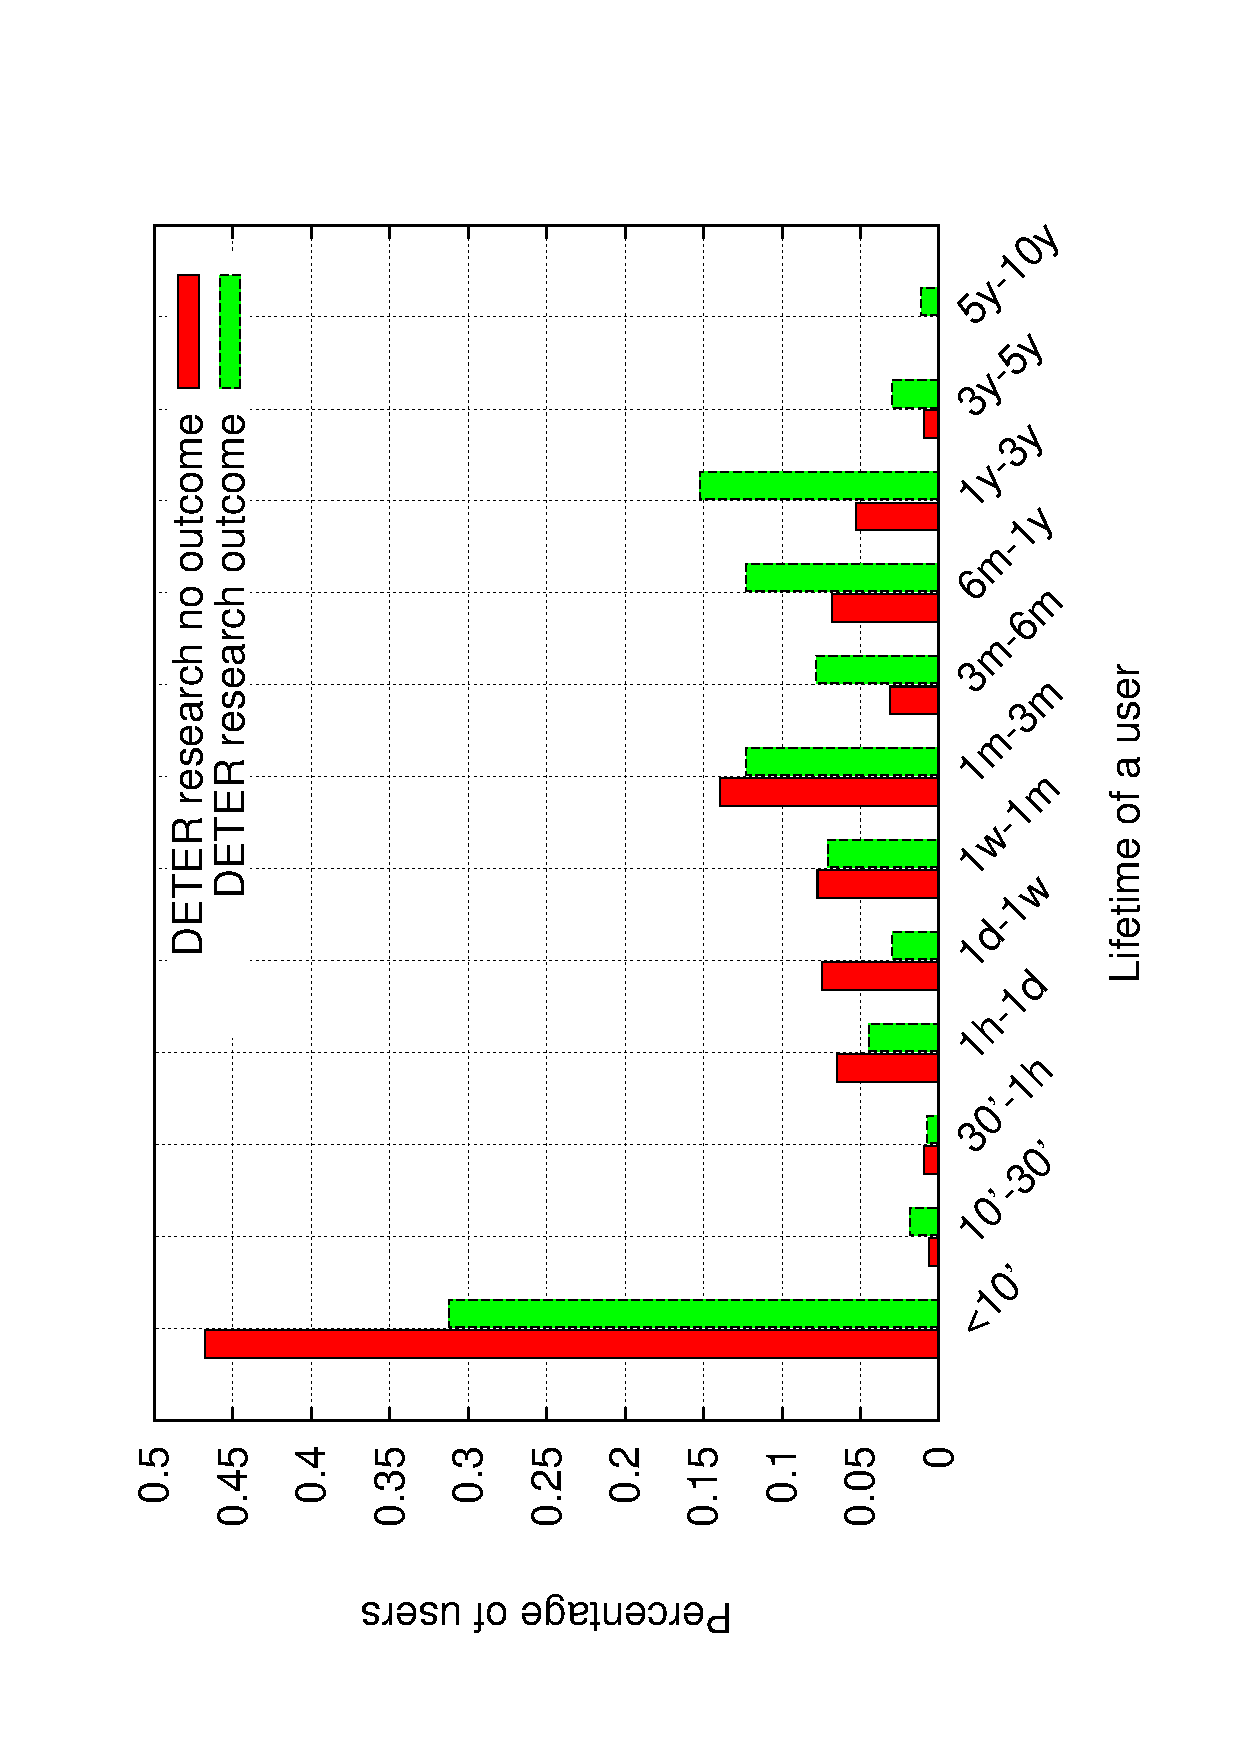
\includegraphics[width=3in,
type=pdf,ext=.pdf,read=.pdf]{figs/user.life.cmp.gnu} \caption{User
lifetime. Left: DETER vs Emulab, Right: All vs outcome} \label{userlife}
\end{center} \end{figure*}


\begin{figure*}[htbp] \begin{center} 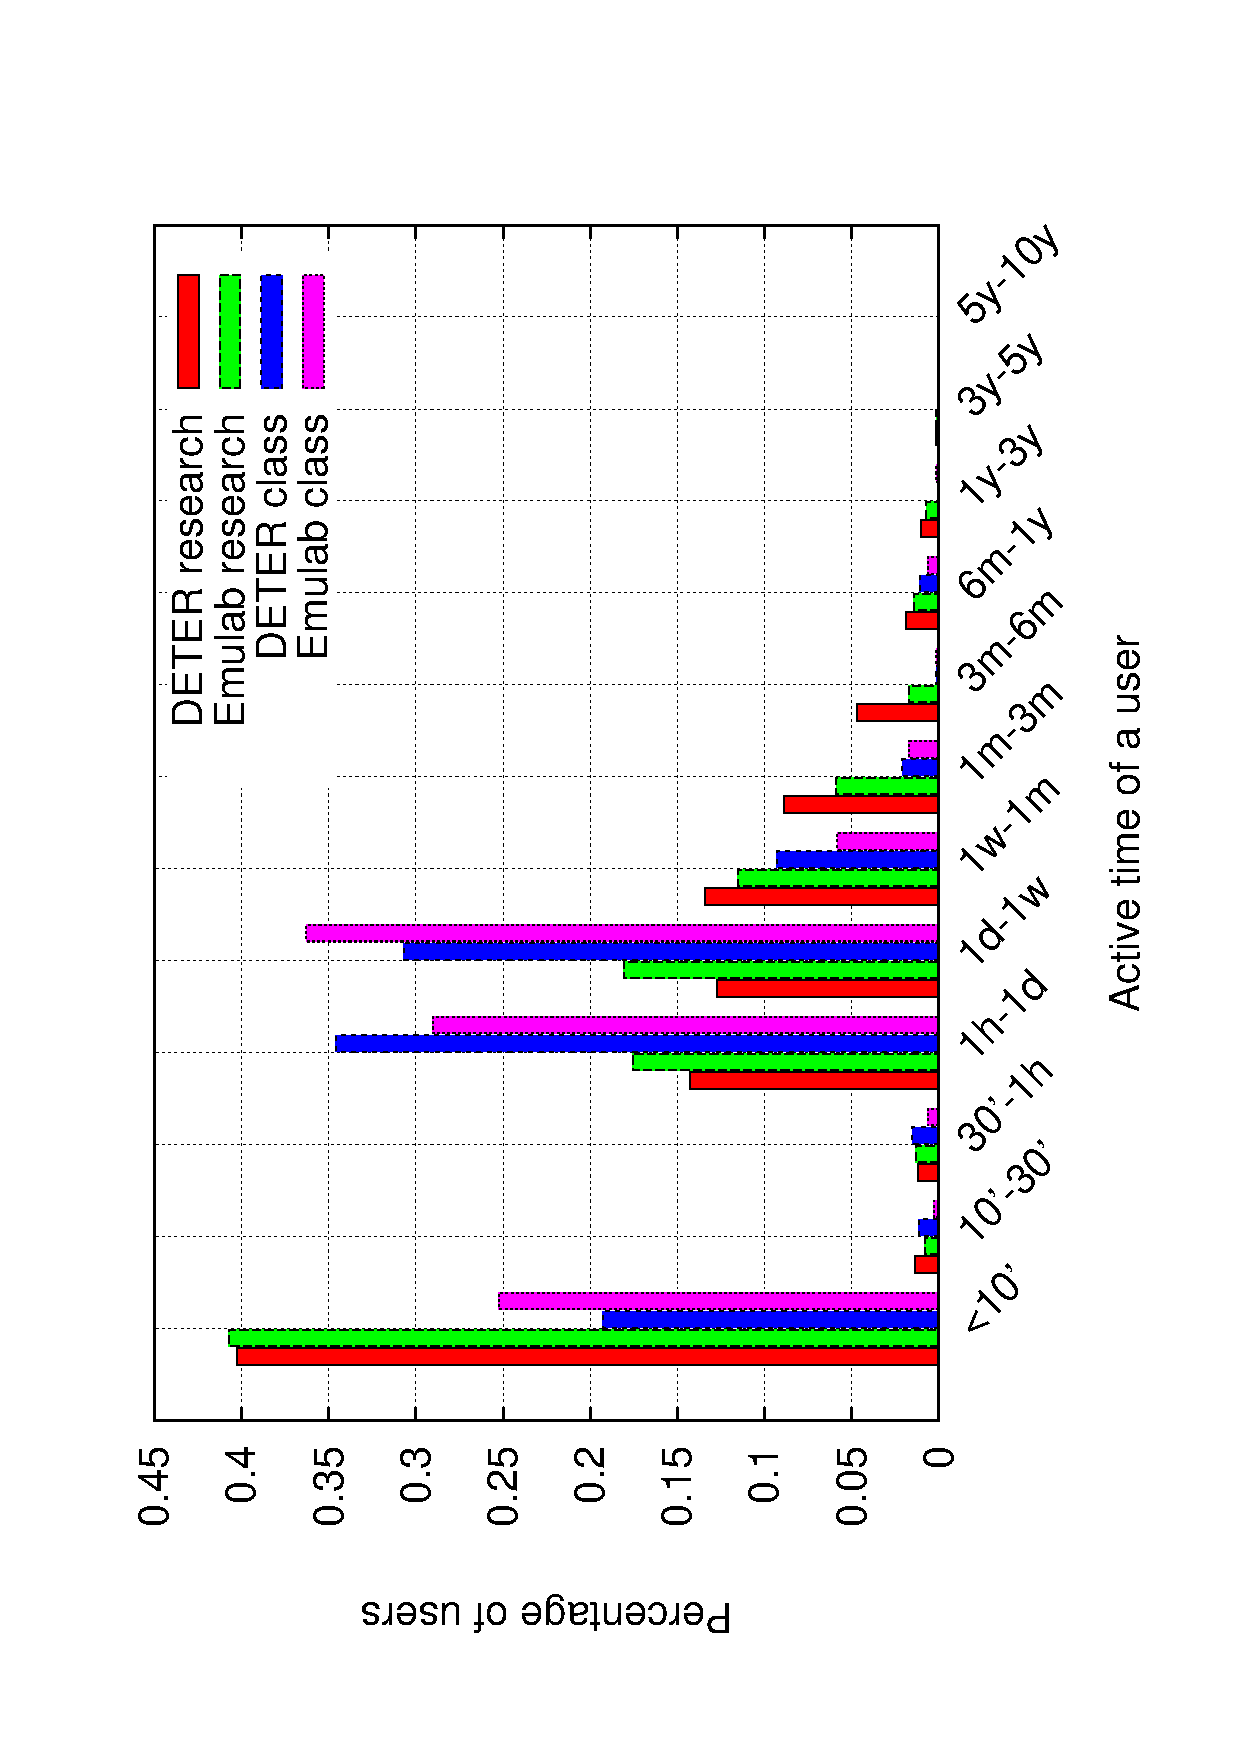
\includegraphics[width=3in,
type=pdf,ext=.pdf,read=.pdf]{figs/user.active.gnu}
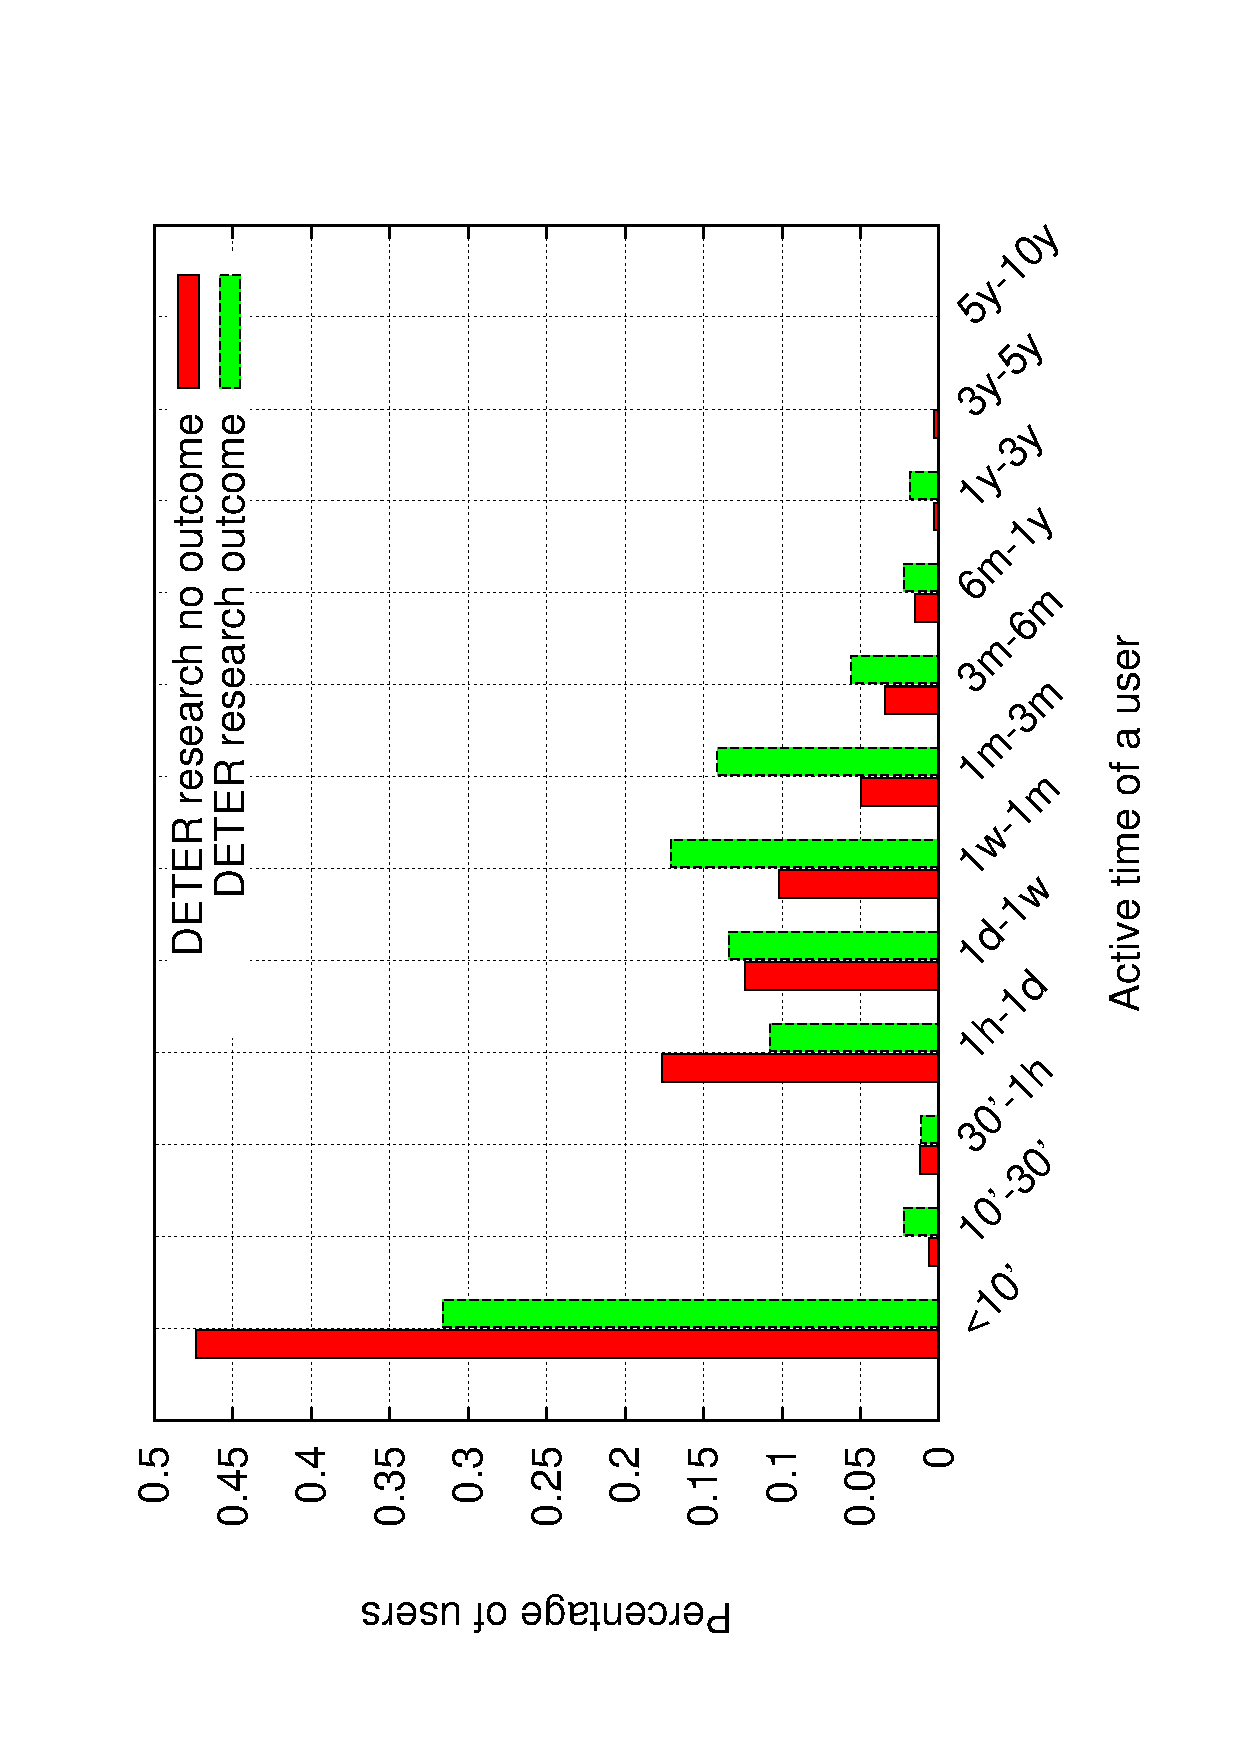
\includegraphics[width=3in,
type=pdf,ext=.pdf,read=.pdf]{figs/user.active.cmp.gnu} \caption{User
active time. Left: DETER vs Emulab, Right: All vs outcome}
\label{useractive} \end{center} \end{figure*}

\begin{figure*}[htbp] \begin{center} 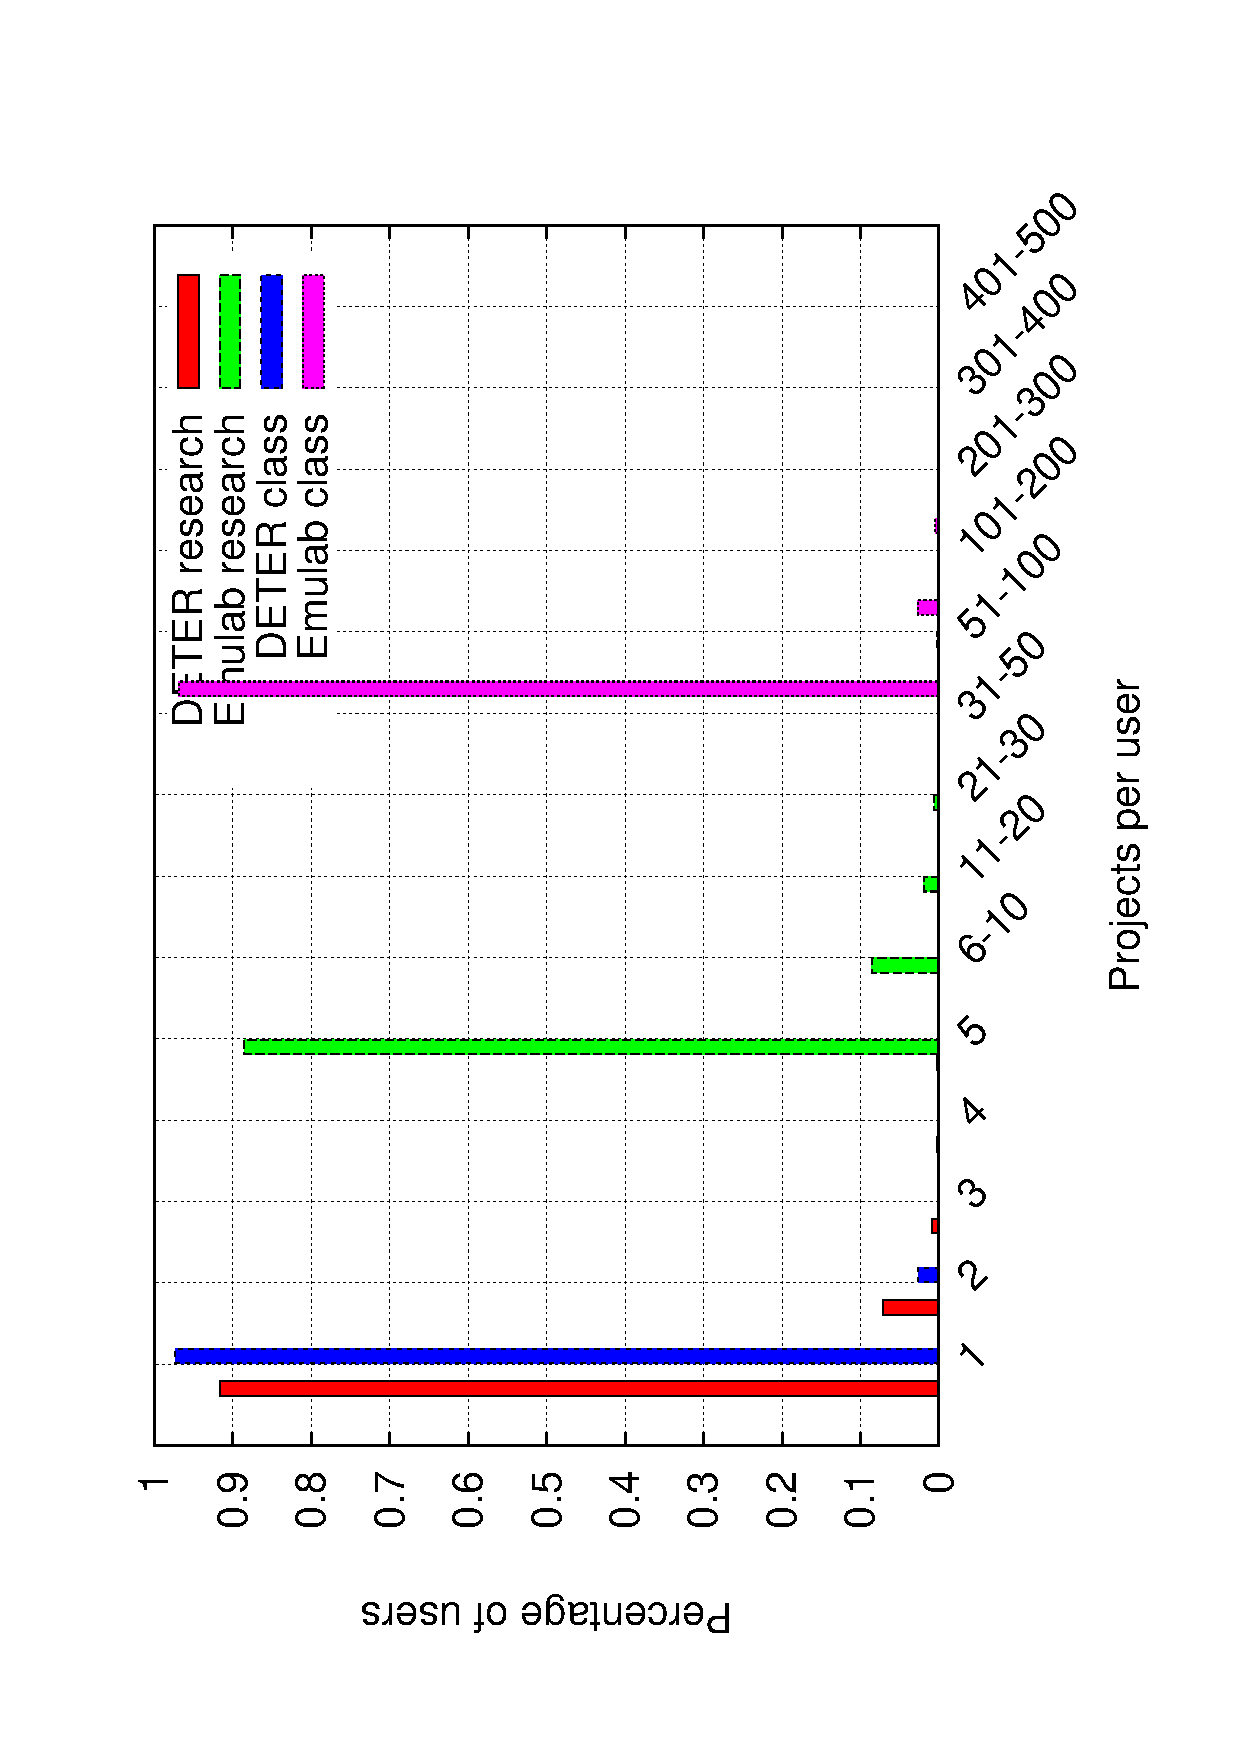
\includegraphics[width=3in,
type=pdf,ext=.pdf,read=.pdf]{figs/user.proj.gnu}
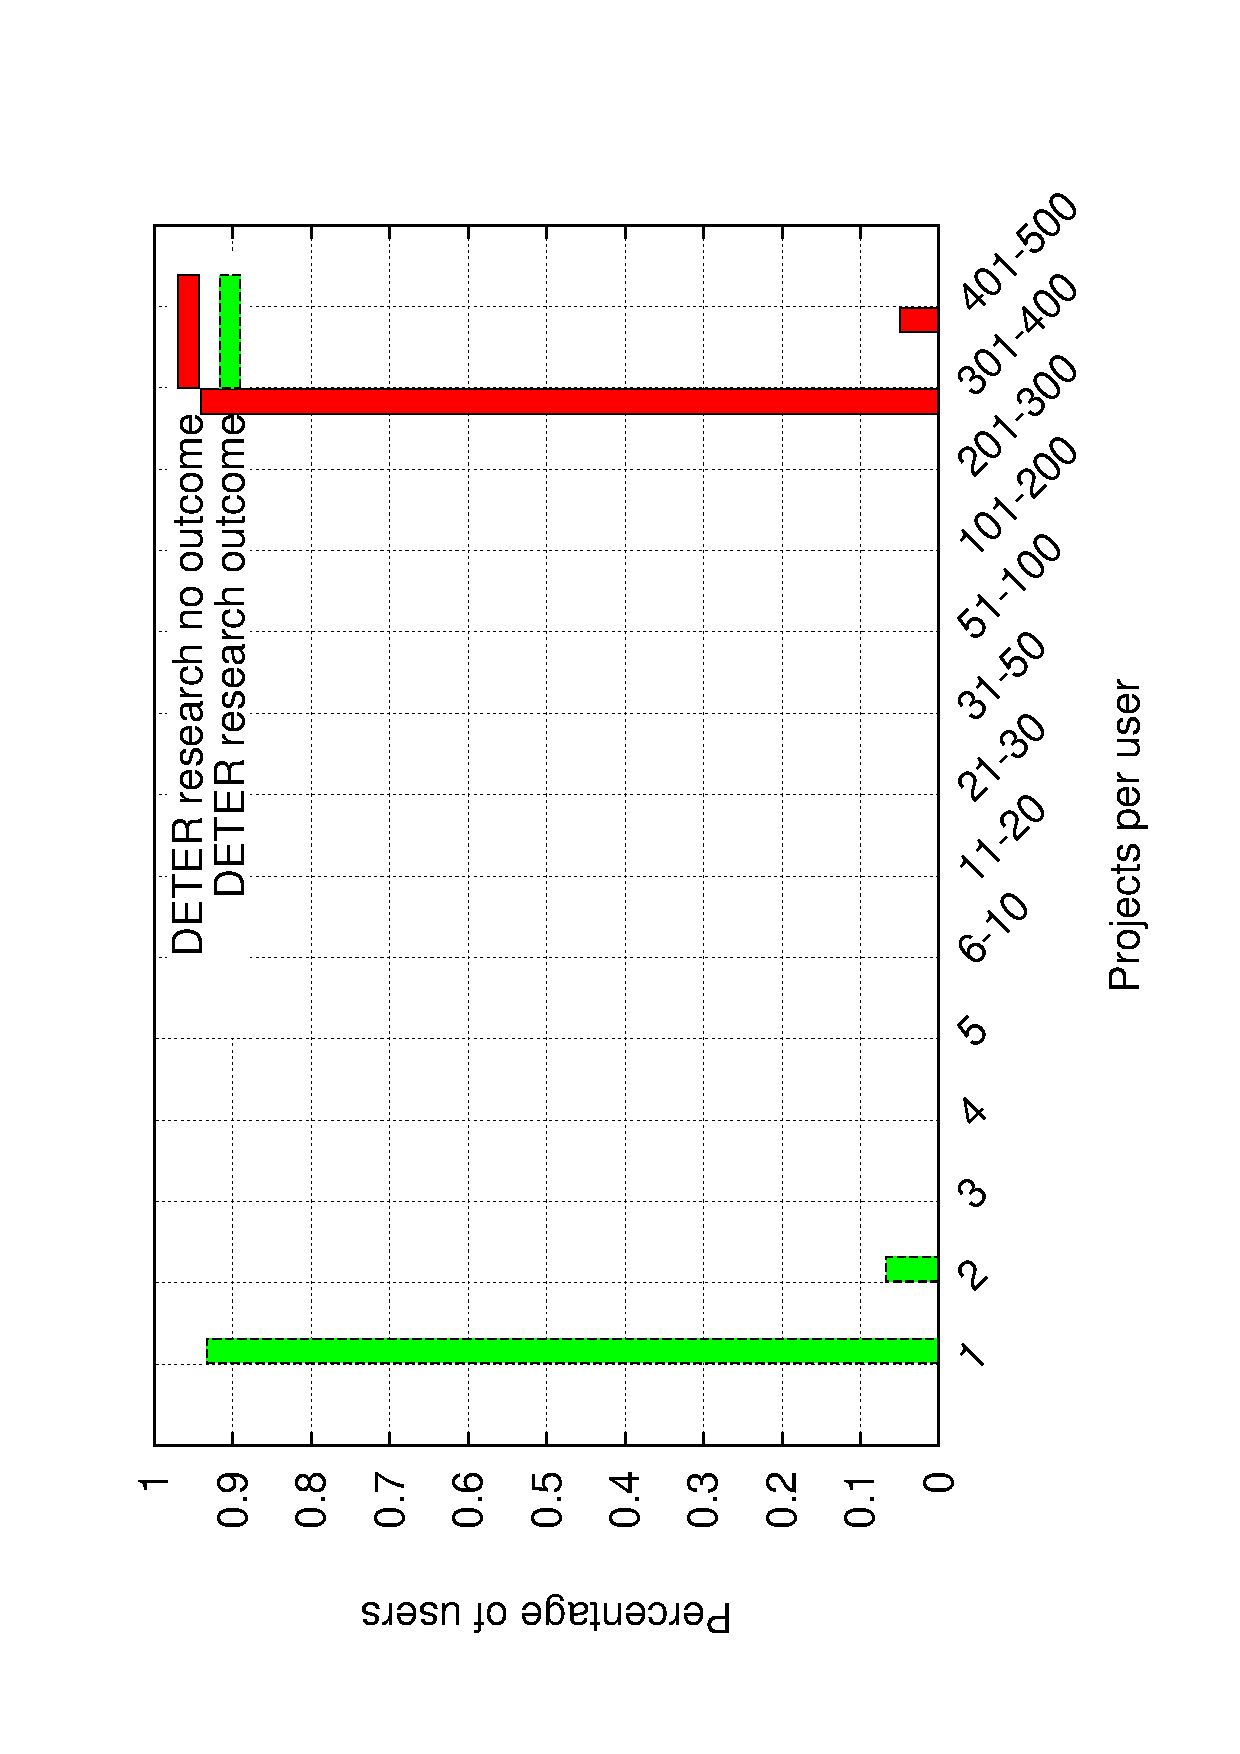
\includegraphics[width=3in,
type=pdf,ext=.pdf,read=.pdf]{figs/user.proj.cmp.gnu} \caption{Projects
per user. Left: DETER vs Emulab, Right: All vs outcome} \label{userproj}
\end{center} \end{figure*}

Members can be deleted and we don't account for that



\subsection{Geolocation Distribution} 



\begin{table}[htdp] \caption{Node activity} \begin{center}
\begin{tabular}{|c|c|} \hline Activity & Percentage \\ \hline Idle &
57\% \\ Network & 30\% \\ CPU & 10\\ Interactive & 3 \\ \hline
\end{tabular} \end{center} \label{default} \end{table}%

57\% of timeslots reported by allocated node were idle but per
experiment all nodes are used together. There are really no huge
inactive periods so inactivity is spread through the experiment. 26\% of
timeslots report a network activity. 6.8\% report a CPU activity and 2\%
report a CPU and network activity.

\begin{figure*}[htbp] \begin{center} 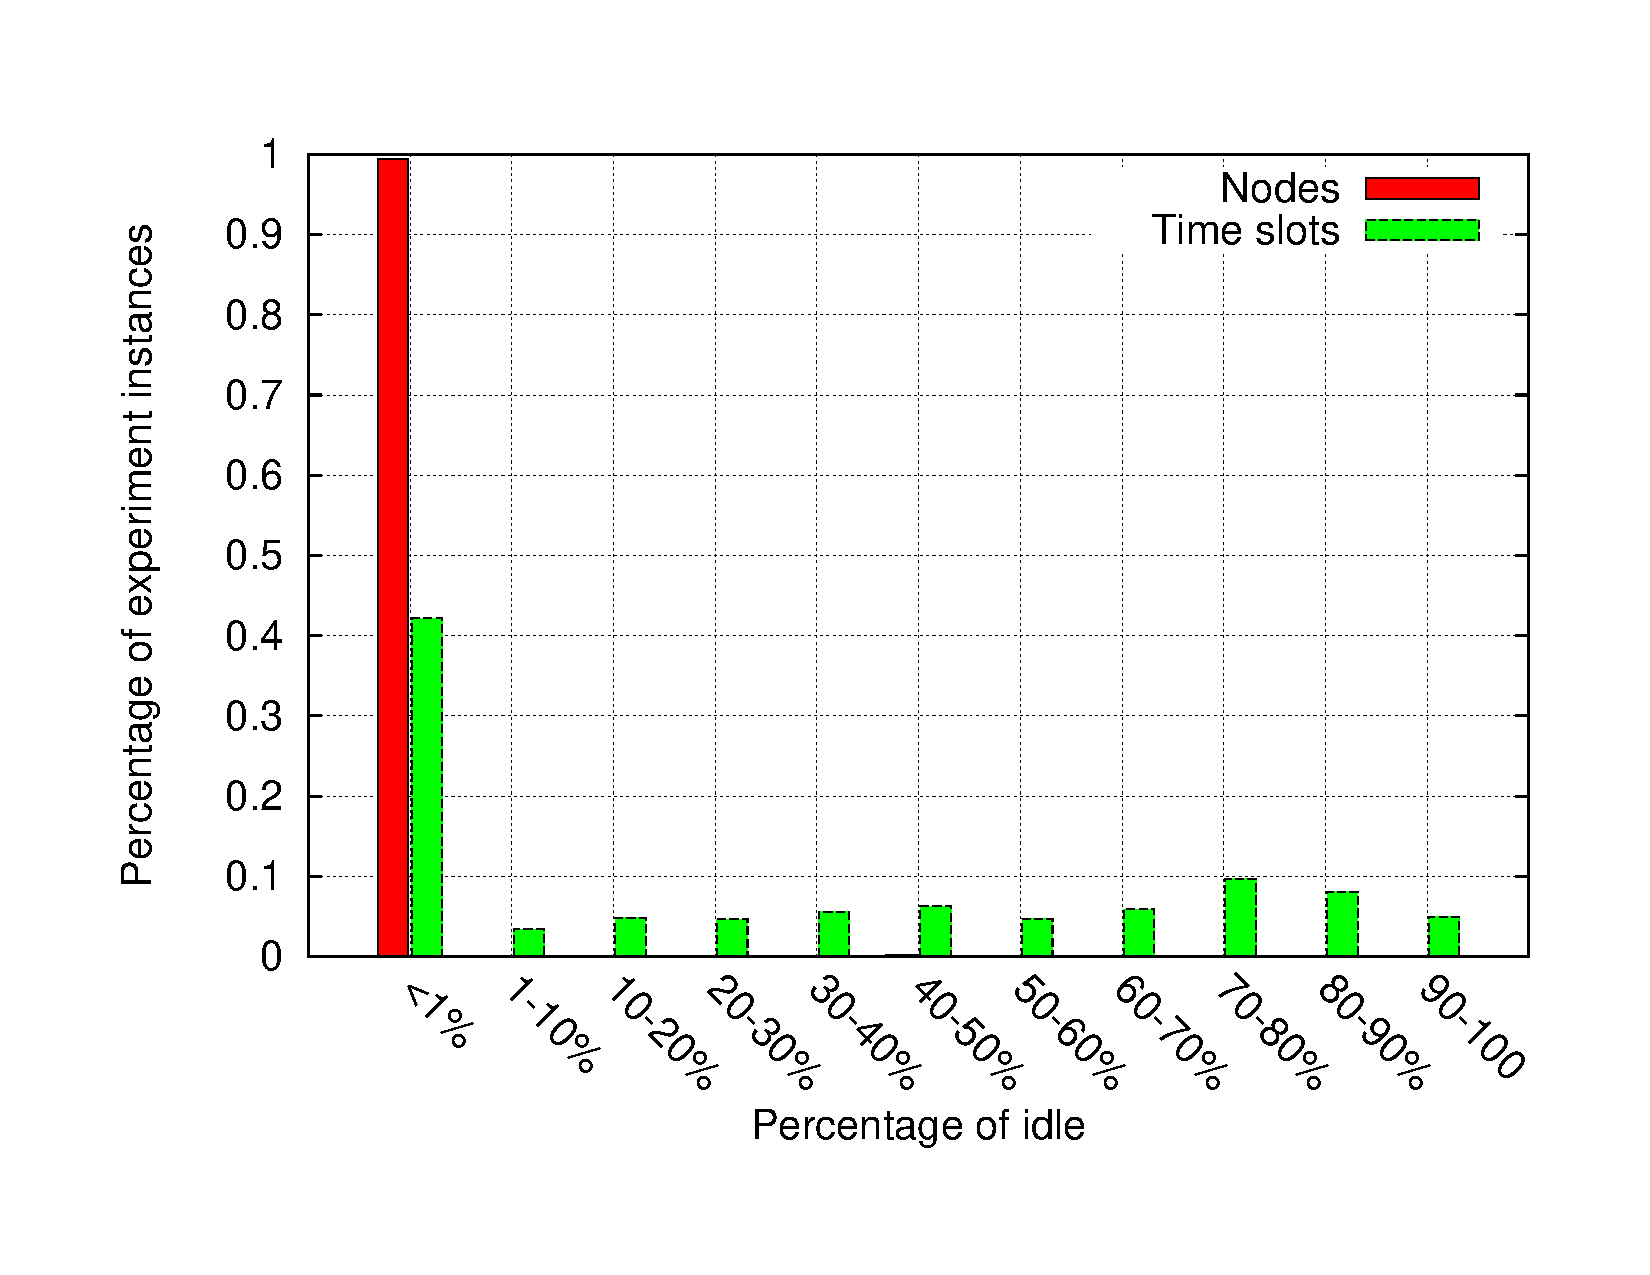
\includegraphics[width=3in,
type=pdf,ext=.pdf,read=.pdf]{figs/exp.idle.gnu}
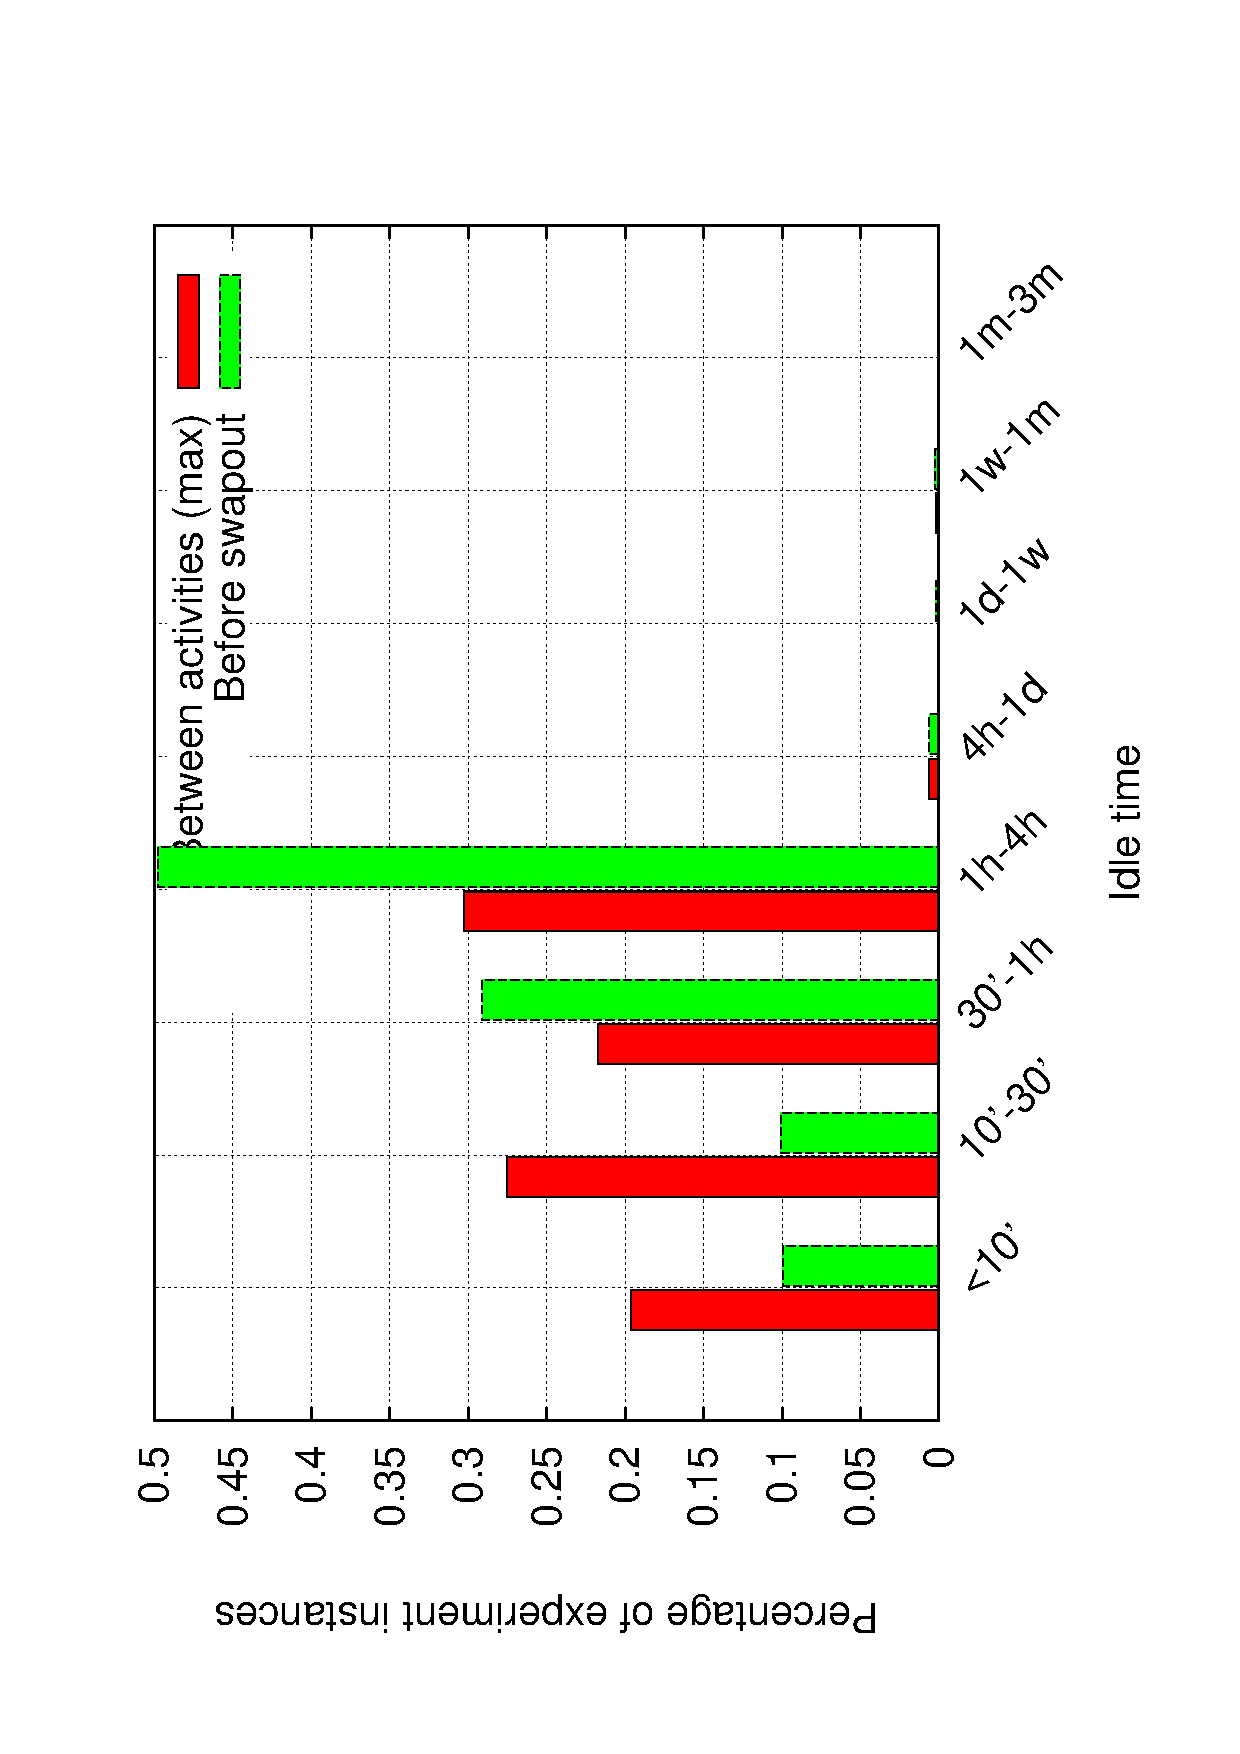
\includegraphics[width=3in,
type=pdf,ext=.pdf,read=.pdf]{figs/period.idle.gnu} \caption{Idleness per
experiment} \label{idle} \end{center} \end{figure*}


cummulative per project idle nodes correlate with experiment duration?
correlate with experiment history?



\section{Functional Patterns}
\label{sec:function}

Per category, what are the functional uses 



\begin{figure*}[htbp] \begin{center}
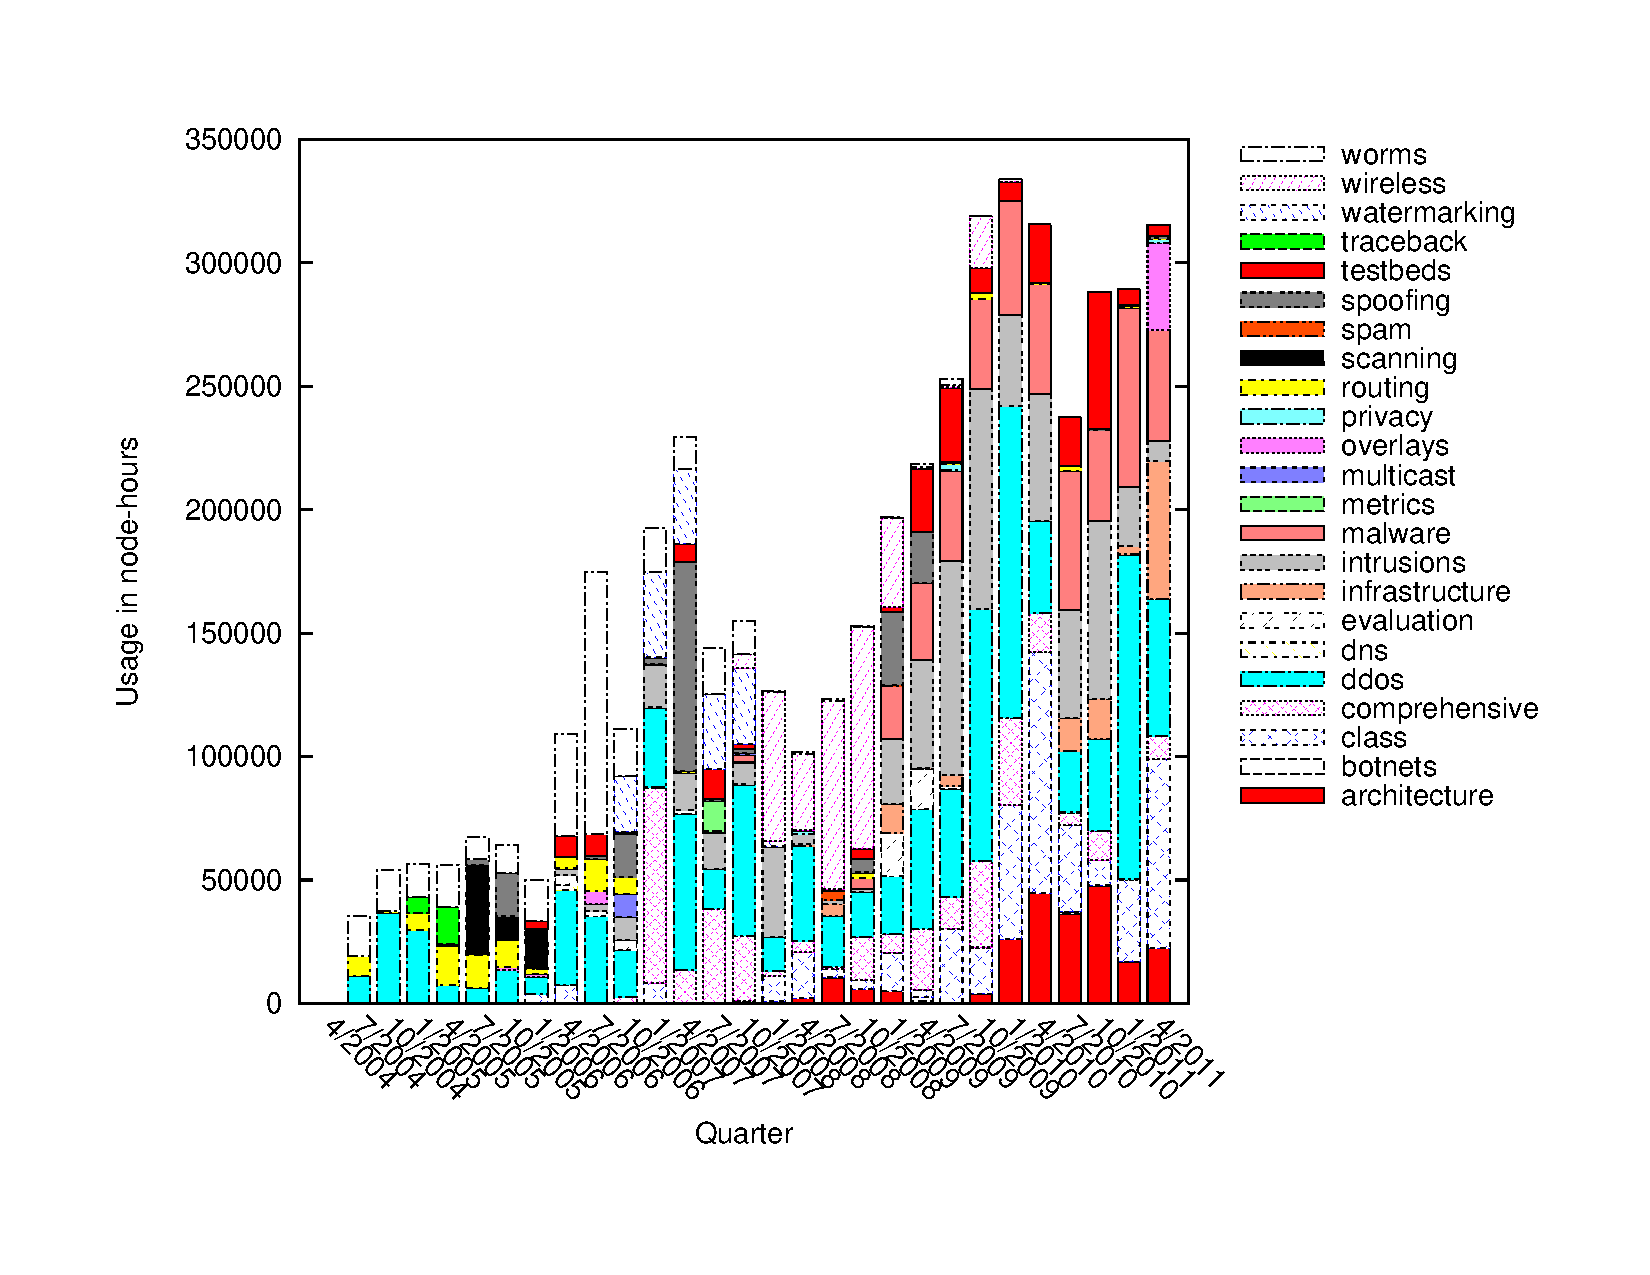
\includegraphics[width=6in,type=pdf,ext=.pdf,read=.pdf]{figs/cat.usage.gnu} \caption{Usage per project category in node-hours in DETER}
\label{catusage} \end{center} \end{figure*}

\begin{figure*}[htbp] \begin{center}
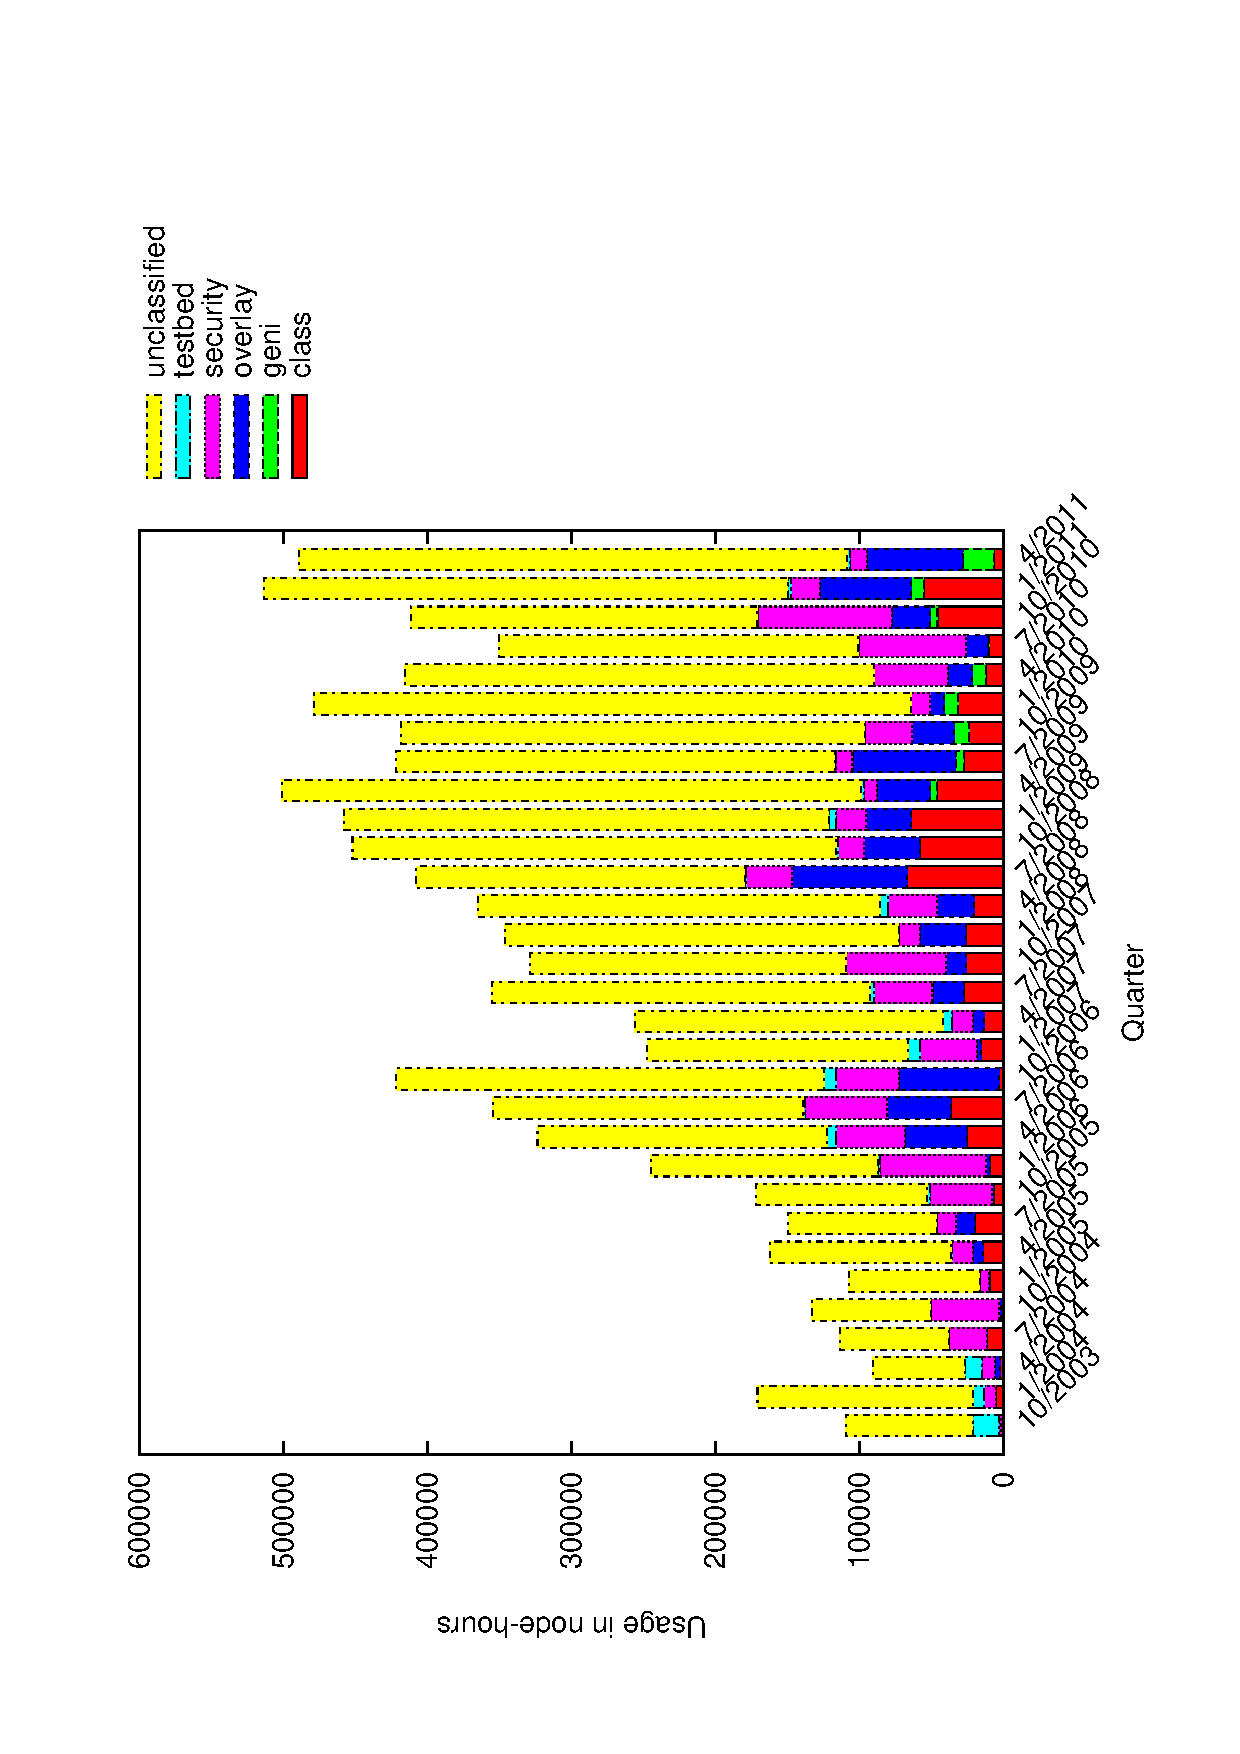
\includegraphics[width=6in,type=pdf,ext=.pdf,read=.pdf]{figs/cat.usage.emu.gnu} \caption{Usage per project category in node-hours in Emulab}
\label{catusage} \end{center} \end{figure*}

%\input{evaluation}
\section{Conclusion} 
\label{sec:conclusion}


\bibliographystyle{plain}
\bibliography{paper}

\end{document}
